% Options for packages loaded elsewhere
\PassOptionsToPackage{unicode}{hyperref}
\PassOptionsToPackage{hyphens}{url}
%
\documentclass[
]{book}
\usepackage{lmodern}
\usepackage{amssymb,amsmath}
\usepackage{ifxetex,ifluatex}
\ifnum 0\ifxetex 1\fi\ifluatex 1\fi=0 % if pdftex
  \usepackage[T1]{fontenc}
  \usepackage[utf8]{inputenc}
  \usepackage{textcomp} % provide euro and other symbols
\else % if luatex or xetex
  \usepackage{unicode-math}
  \defaultfontfeatures{Scale=MatchLowercase}
  \defaultfontfeatures[\rmfamily]{Ligatures=TeX,Scale=1}
\fi
% Use upquote if available, for straight quotes in verbatim environments
\IfFileExists{upquote.sty}{\usepackage{upquote}}{}
\IfFileExists{microtype.sty}{% use microtype if available
  \usepackage[]{microtype}
  \UseMicrotypeSet[protrusion]{basicmath} % disable protrusion for tt fonts
}{}
\makeatletter
\@ifundefined{KOMAClassName}{% if non-KOMA class
  \IfFileExists{parskip.sty}{%
    \usepackage{parskip}
  }{% else
    \setlength{\parindent}{0pt}
    \setlength{\parskip}{6pt plus 2pt minus 1pt}}
}{% if KOMA class
  \KOMAoptions{parskip=half}}
\makeatother
\usepackage{xcolor}
\IfFileExists{xurl.sty}{\usepackage{xurl}}{} % add URL line breaks if available
\IfFileExists{bookmark.sty}{\usepackage{bookmark}}{\usepackage{hyperref}}
\hypersetup{
  pdftitle={Advanced Psychological Research Methods (PSY4034)},
  pdfauthor={Christopher J. Wilson},
  hidelinks,
  pdfcreator={LaTeX via pandoc}}
\urlstyle{same} % disable monospaced font for URLs
\usepackage{color}
\usepackage{fancyvrb}
\newcommand{\VerbBar}{|}
\newcommand{\VERB}{\Verb[commandchars=\\\{\}]}
\DefineVerbatimEnvironment{Highlighting}{Verbatim}{commandchars=\\\{\}}
% Add ',fontsize=\small' for more characters per line
\usepackage{framed}
\definecolor{shadecolor}{RGB}{248,248,248}
\newenvironment{Shaded}{\begin{snugshade}}{\end{snugshade}}
\newcommand{\AlertTok}[1]{\textcolor[rgb]{0.94,0.16,0.16}{#1}}
\newcommand{\AnnotationTok}[1]{\textcolor[rgb]{0.56,0.35,0.01}{\textbf{\textit{#1}}}}
\newcommand{\AttributeTok}[1]{\textcolor[rgb]{0.77,0.63,0.00}{#1}}
\newcommand{\BaseNTok}[1]{\textcolor[rgb]{0.00,0.00,0.81}{#1}}
\newcommand{\BuiltInTok}[1]{#1}
\newcommand{\CharTok}[1]{\textcolor[rgb]{0.31,0.60,0.02}{#1}}
\newcommand{\CommentTok}[1]{\textcolor[rgb]{0.56,0.35,0.01}{\textit{#1}}}
\newcommand{\CommentVarTok}[1]{\textcolor[rgb]{0.56,0.35,0.01}{\textbf{\textit{#1}}}}
\newcommand{\ConstantTok}[1]{\textcolor[rgb]{0.00,0.00,0.00}{#1}}
\newcommand{\ControlFlowTok}[1]{\textcolor[rgb]{0.13,0.29,0.53}{\textbf{#1}}}
\newcommand{\DataTypeTok}[1]{\textcolor[rgb]{0.13,0.29,0.53}{#1}}
\newcommand{\DecValTok}[1]{\textcolor[rgb]{0.00,0.00,0.81}{#1}}
\newcommand{\DocumentationTok}[1]{\textcolor[rgb]{0.56,0.35,0.01}{\textbf{\textit{#1}}}}
\newcommand{\ErrorTok}[1]{\textcolor[rgb]{0.64,0.00,0.00}{\textbf{#1}}}
\newcommand{\ExtensionTok}[1]{#1}
\newcommand{\FloatTok}[1]{\textcolor[rgb]{0.00,0.00,0.81}{#1}}
\newcommand{\FunctionTok}[1]{\textcolor[rgb]{0.00,0.00,0.00}{#1}}
\newcommand{\ImportTok}[1]{#1}
\newcommand{\InformationTok}[1]{\textcolor[rgb]{0.56,0.35,0.01}{\textbf{\textit{#1}}}}
\newcommand{\KeywordTok}[1]{\textcolor[rgb]{0.13,0.29,0.53}{\textbf{#1}}}
\newcommand{\NormalTok}[1]{#1}
\newcommand{\OperatorTok}[1]{\textcolor[rgb]{0.81,0.36,0.00}{\textbf{#1}}}
\newcommand{\OtherTok}[1]{\textcolor[rgb]{0.56,0.35,0.01}{#1}}
\newcommand{\PreprocessorTok}[1]{\textcolor[rgb]{0.56,0.35,0.01}{\textit{#1}}}
\newcommand{\RegionMarkerTok}[1]{#1}
\newcommand{\SpecialCharTok}[1]{\textcolor[rgb]{0.00,0.00,0.00}{#1}}
\newcommand{\SpecialStringTok}[1]{\textcolor[rgb]{0.31,0.60,0.02}{#1}}
\newcommand{\StringTok}[1]{\textcolor[rgb]{0.31,0.60,0.02}{#1}}
\newcommand{\VariableTok}[1]{\textcolor[rgb]{0.00,0.00,0.00}{#1}}
\newcommand{\VerbatimStringTok}[1]{\textcolor[rgb]{0.31,0.60,0.02}{#1}}
\newcommand{\WarningTok}[1]{\textcolor[rgb]{0.56,0.35,0.01}{\textbf{\textit{#1}}}}
\usepackage{longtable,booktabs}
% Correct order of tables after \paragraph or \subparagraph
\usepackage{etoolbox}
\makeatletter
\patchcmd\longtable{\par}{\if@noskipsec\mbox{}\fi\par}{}{}
\makeatother
% Allow footnotes in longtable head/foot
\IfFileExists{footnotehyper.sty}{\usepackage{footnotehyper}}{\usepackage{footnote}}
\makesavenoteenv{longtable}
\usepackage{graphicx,grffile}
\makeatletter
\def\maxwidth{\ifdim\Gin@nat@width>\linewidth\linewidth\else\Gin@nat@width\fi}
\def\maxheight{\ifdim\Gin@nat@height>\textheight\textheight\else\Gin@nat@height\fi}
\makeatother
% Scale images if necessary, so that they will not overflow the page
% margins by default, and it is still possible to overwrite the defaults
% using explicit options in \includegraphics[width, height, ...]{}
\setkeys{Gin}{width=\maxwidth,height=\maxheight,keepaspectratio}
% Set default figure placement to htbp
\makeatletter
\def\fps@figure{htbp}
\makeatother
\setlength{\emergencystretch}{3em} % prevent overfull lines
\providecommand{\tightlist}{%
  \setlength{\itemsep}{0pt}\setlength{\parskip}{0pt}}
\setcounter{secnumdepth}{5}
\usepackage{booktabs}
\usepackage{booktabs}
\usepackage{longtable}
\usepackage{array}
\usepackage{multirow}
\usepackage{wrapfig}
\usepackage{float}
\usepackage{colortbl}
\usepackage{pdflscape}
\usepackage{tabu}
\usepackage{threeparttable}
\usepackage{threeparttablex}
\usepackage[normalem]{ulem}
\usepackage{makecell}
\usepackage[]{natbib}
\bibliographystyle{apalike}

\title{Advanced Psychological Research Methods (PSY4034)}
\author{Christopher J. Wilson}
\date{2020-09-10}

\begin{document}
\maketitle

{
\setcounter{tocdepth}{1}
\tableofcontents
}
\hypertarget{welcome-to-the-module}{%
\chapter{Welcome to the module}\label{welcome-to-the-module}}

\begin{quote}
Note: You should be able to see a video immediately below this text. To watch the video, you will need to be logged into Teesside University's Blackboard site and be a part of this course. If you are on the course:

\begin{itemize}
\tightlist
\item
  Press \emph{Ctrl} + \emph{T} to open a new tab (keeping this one open) and go to \url{https://eat.tees.ac.uk}.
\item
  Login to Blackboard. Keep the blackboard tab open and switch back to this page.
\item
  Refresh this page (hit F5 on your keyboard).
\item
  You should now be able to play all of the video content.
\end{itemize}
\end{quote}

\hypertarget{module-overview}{%
\section{Module Overview}\label{module-overview}}

This Level 7 module for first year Doctorate in Clinical Psychology trainees aims to enable you to:

\begin{itemize}
\tightlist
\item
  Refresh and extend your knowledge, skills and critical understanding of advanced research methods using both qualitative and quantitative approaches;
\item
  Creatively apply the principles of quantitative and qualitative research methods to clinical psychology research and practice;
\item
  Refresh and extend your skills in project design, management, analysis and presentation.
\end{itemize}

The module is also designed to explicitly prepare you for the two Doctorate level research modules which occur in Years Two and Three of the programme, ensuring that you have the requisite knowledge and skills to successfully engage with those modules.

The key foci for this module include:

\begin{itemize}
\tightlist
\item
  critical review of established literature
\item
  project design
\item
  project management
\item
  data analysis
\item
  dissemination of research findings
\end{itemize}

The module is taught using a variety of techniques to best enhance your knowledge and understanding of the application of research theory and methods in the context of clinical psychology. These include lectures, seminars, guided statistical analysis and tutorials with the latter being used to provide individual guidance and formative feedback. The module has its own site on the University's Virtual Learning Environment \url{http://eat.tees.ac.uk} - known as Blackboard), with resources and literature designed to support learning.

\hypertarget{module-timetable-and-delivery-for-20202021}{%
\section{Module timetable and delivery for 2020/2021}\label{module-timetable-and-delivery-for-20202021}}

The timetable for this module appears on the Clinical Psychology Programme Site/Timetables.
The majority of the sessions will take place on Monday mornings. Please note that the timetable should be checked on a regular basis.

\textbf{Due to COVID19 pandemic, the sessions for this module will be delivered online in 2020/21}

\hypertarget{learning-and-teaching-strategies}{%
\subsection{Learning and Teaching Strategies}\label{learning-and-teaching-strategies}}

The module is taught using a variety of techniques to best enhance your knowledge and understanding of the application of research theory and methods in the context of clinical psychology. This includes activities designed to encourage independent learning, a key skill for successful performance in research modules in Years Two and Three of the programme. Evidence of independent learning is expected in the assignments for this module. Specific links are made with research informed activity in practice.

You will be provided with two papers for critical review at the start of the module and asked to decide which one you will use for your summative critical review assignment; one of these papers is from a quantitative research tradition and the other is from a qualitative research tradition.

All presentations (with added annotations) are available, along with additional support materials, via an \href{mailto:e-learning@tees}{\nolinkurl{e-learning@tees}} on the VLE. E-learning is enabled through group activities on the VLE or Microsoft Teams where discussion and problem solving is undertaken in relation to tasks set during teaching sessions. The discussion boards or Microsoft Teams site will be used to ask and answer questions that arise from the taught material and also your independent work.

\hypertarget{how-will-the-online-sessions-work}{%
\subsection{How will the online sessions work?}\label{how-will-the-online-sessions-work}}

The video below explains how online sessions will work:

\hypertarget{assessment}{%
\section{Assessment}\label{assessment}}

\hypertarget{formative-assessment}{%
\subsection{Formative assessment}\label{formative-assessment}}

Formative feedback is provided throughout the module through practical exercises and in seminars on trainee presentations.

By the end of year one, trainees are expected to have identified a thesis topic and have a completed research proposal. As such, there are a number of formative milestones across the year that will be monitored by the module team. Please see Appendix 1 of this guide for details.

The required format for thesis research proposals can be found in Appendix 2 of the DClinPsy
Programme Research Handbook.

\textbf{The formal formative assessment is of a presentation of the thesis research proposal to be presented during the research panels, which take place on 20, 21 and 22 July 2020.} The presentation will be 20 minutes' long and will outline the thesis project that the trainee will develop in Years 2 and 3. There will also be 10 minutes allotted for questions from the panel which will have two academic members and one clinical member. This formative assessment is intended as a starting point for the Year 2 and 3 research methods modules. The timing is important as it should enable trainees to start the process of ethics approval for their dissertation. earlier. The trainees will hand in a printed copy of their slides with explanatory notes and references.

\textbf{Formative Assessment Criteria}

The following criteria will be used to assess the assignment:

\begin{itemize}
\tightlist
\item
  Effective justification for the study.
\item
  Clearly defined research question.
\item
  Comprehensive and critical review of the literature (within time constraints).
\item
  Realistic research design.
\item
  Effective consideration of ethical issues.
\item
  Clear plan for writing up and dissemination.
\item
  Fulfilment of professional research ethics requirements.
\item
  Adherence to the relevant guidance for presentation as advised by the Module Tutor.
\end{itemize}

\hypertarget{summative-assessments}{%
\subsection{Summative Assessments}\label{summative-assessments}}

Assessment consists of an ICA and an ECA, each worth 50\% of the overall module mark. The deadlines for these assessments can be found in the assessments section on Blackboard or in the programme assessment timetable.

\textbf{ICA (50\%)} - A critical review of a published primary research paper (choice to be made by a trainee from three papers with different methodologies provided by the tutor). One of these papers is from a quantitative research approach, one from a qualitative research approach and the third will use mixed methods (2,000 words).
\emph{Learning outcomes: (KU 1-4, CIS 1-3, KTS 1-3)}

\textbf{ICA Assessment Criteria (Critical Appraisal of Published Primary Research Paper )}

The following criteria will be used to assess the assignment:

\begin{itemize}
\tightlist
\item
  Demonstrate a critical understanding of the role of the reviewed paper for clinical psychologists in service delivery and/or practice.
\item
  Demonstrate a critical and comprehensive understanding of the relevant methodological issues.
\item
  Systematically and critically evaluate stages of the research process.
\item
  Demonstrate a comprehensive and critical understanding of the ethical issues involved in the research.
\item
  Reach effectively argued conclusions.
\item
  Demonstrate independent learning ability through reflection on the critical review process.
\item
  Adhere to the American Psychological Association (APA) guidelines for presentation and referencing.
\end{itemize}

\textbf{ECA (50\%)} - A research project proposal which both addresses limitations identified in the ICA critical review (1) and develops the research further with the use of an alternative methodology (2,000 words).\\
\emph{Learning outcomes: (KU 1-4, CIS 1-3, PPS 1-2, KTS 1-5)}

\textbf{ECA Assessment Criteria (Research Project Proposal)}

The following criteria will be used to assess the assignment:

\begin{itemize}
\tightlist
\item
  Identify a project that demonstrates a detailed and critical understanding of the research evidence reviewed and wider methodological issues, including the role of the project for informing service delivery and/or practice.
\item
  Provide detailed and appropriately justified solutions to the design of the research project.
\item
  Consider both methodological and ethical issues in the design of the research project.
\item
  Demonstrate a detailed and critical understanding of the data analysis required for the proposed study.
\item
  Adhere to the American Psychological Association (APA) guidelines for presentation and referencing.
\end{itemize}

\hypertarget{word-limits-for-assessment}{%
\subsection{Word limits for assessment}\label{word-limits-for-assessment}}

Word limits are as stated above (note that there is no allowance of +10\%). The word count refers to the assignment itself and does not include the reference list or tables/graphs. The references cited in the main body of text are included in the word count.

\hypertarget{submitting-work}{%
\subsection{Submitting work}\label{submitting-work}}

All work should be submitted electronically, using the apporpriate links on the module Blackboard site. A printed hard copy of the assignment is \textbf{not} required and should not be submitted. \textbf{The university's policy is that all assessments must be submitted by 4 p.m. on the day of the deadline.}

\hypertarget{a-note-about-referencing}{%
\subsection{A note about referencing}\label{a-note-about-referencing}}

There is an expectation that all academic assignments conform to current American Psychological Association referencing and citation conventions. Poor referencing will be taken into consideration when marking. It is recommended that you use a digital reference management system (e.g., Refworks, Mendley), which are freely available (and will save you time). The following online resources are also useful:

\url{http://reciteworks.com/} - good for checking fine details (e.g., missing references)

\url{http://www.apastyle.org} - detailed guidance for APA style

\url{https://owl.english.purdue.edu/owl/resource/560/01/}- additional advice for APA style

\hypertarget{statistical-analysis-software}{%
\section{Statistical analysis software}\label{statistical-analysis-software}}

You may be familiar with SPSS from your undergraduate statistics teaching. Please note that we do not use SPSS for teaching and instead use R Statistics. The reason for this is that R is a free statistical package, meaning that it can be accessed in NHS settings that do not have funding for SPSS. This will enable you to run statistical analyses whilst on placement where required, and also enables you to conduct statistical analyses as a qualified Psychologist without incurring any software costs. R is also more flexible than SPSS and has greater functionality. During the teaching you will be shown how to set up and install R, and how to run statistical analyses in this software.

\hypertarget{downloading-r-and-r-studio}{%
\subsection{Downloading R and R Studio}\label{downloading-r-and-r-studio}}

You can obtain R and R Studio from the following links:

\url{https://cran.r-project.org/}

\url{https://rstudio.com/}

\hypertarget{academic-support-and-guidance}{%
\section{Academic Support and Guidance}\label{academic-support-and-guidance}}

Please contact the module team if you have any questions, concerns or any other areas you wish to discuss.

\hypertarget{module-team-contact-details}{%
\subsection{Module Team Contact Details}\label{module-team-contact-details}}

Module Leader: Dr Christopher Wilson: \href{mailto:christopher.wilson@tees.ac.uk}{\nolinkurl{christopher.wilson@tees.ac.uk}}

Module Team: Dr Alan Bowman: \href{mailto:A.Bowman@tees.ac.uk}{\nolinkurl{A.Bowman@tees.ac.uk}}

Guest lecturers from Schools within the University and Local NHS clinicians also contribute to some teaching

\hypertarget{considering-your-thesis}{%
\section{Considering your thesis}\label{considering-your-thesis}}

Your doctoral thesis is one of the largest pieces of work you will undertake during your training and it is important to start thinking about it early on.

You are advised to read around the area of your thesis topic on a continuing basis, and make use of tutorials with your supervision team when needed.

It is also advised that you consider research governance and ethics as you develop your project. Please speak to your academic supervisor about this as they will be able to advise or direct you to someone with appropriate expertise to address queries.

As specified in the Research Handbook, \textbf{please note that a revised version of your research proposal forms one of your year two summative assignments}. The deadline for this assignment is \textbf{early on in the start of second year} and it is therefore advised that you work on your revised proposal as soon as you receive feedback from the panels and have discussed this with your academic supervisor.

\hypertarget{research-methods-concepts-revision}{%
\chapter{Research Methods Concepts Revision}\label{research-methods-concepts-revision}}

\hypertarget{basic-concepts-that-you-should-already-know}{%
\section{Basic concepts that you should already know}\label{basic-concepts-that-you-should-already-know}}

\hypertarget{probability-and-hypothesis-testing}{%
\section{Probability and hypothesis testing}\label{probability-and-hypothesis-testing}}

One of the most important things to remember about hypothesis testing in statistics is why we use the approaches we do. That is, we need statistical approaches to test hypotheses because we can only collect data from samples of the population but our research questions and hypotheses apply to whole populations. For that reason, we need a way to estimate how well the \emph{sample} reflects the \emph{population.}

It is common for us to want to know what the mean (average) response of the population is on certain measures. For example, we might ask the question ``what is the average score on this measure of happiness?''. In reality we can only measure a subset (sample) of the population, so we test as many people as we can. Below is a sample of 20 participants:

\begin{verbatim}
## Warning: package 'kableExtra' was built under R version 4.0.2
\end{verbatim}

\begin{verbatim}
## 
## Attaching package: 'kableExtra'
\end{verbatim}

\begin{verbatim}
## The following object is masked from 'package:dplyr':
## 
##     group_rows
\end{verbatim}

\begin{table}

\caption{\label{tab:unnamed-chunk-2}Some sample data for happiness score}
\centering
\begin{tabular}[t]{r|r|r}
\hline
participant & intervention & happiness\\
\hline
1 & 1 & 11.126738\\
\hline
2 & 2 & 11.455096\\
\hline
3 & 1 & 9.448889\\
\hline
4 & 1 & 6.567100\\
\hline
5 & 2 & 11.080759\\
\hline
6 & 1 & 9.866935\\
\hline
7 & 1 & 11.066079\\
\hline
8 & 2 & 7.115263\\
\hline
9 & 1 & 8.478822\\
\hline
10 & 2 & 9.126518\\
\hline
11 & 1 & 11.077905\\
\hline
12 & 2 & 11.238149\\
\hline
13 & 2 & 6.796180\\
\hline
14 & 2 & 7.745382\\
\hline
15 & 1 & 9.542996\\
\hline
16 & 1 & 7.913203\\
\hline
17 & 1 & 9.601031\\
\hline
18 & 1 & 10.571534\\
\hline
19 & 2 & 9.679823\\
\hline
20 & 2 & 12.890654\\
\hline
\end{tabular}
\end{table}

\hypertarget{variance-in-sample-data-influences-our-confidence-in-population-estimates}{%
\section{Variance in sample data influences our confidence in population estimates}\label{variance-in-sample-data-influences-our-confidence-in-population-estimates}}

We can see from the table above that the mean of the sample is 9.6194528. However, this is not to say that the population mean is 9.6194528. For one thing, we can see that the range of scores in the sample is between 6.5671002 and 12.890654. The standard deviation of the sample is 2.

The fact that there is so much variance from person to person within our sample indicates that we are likely to be incorrect if we assume that the sample mean is the same as the population mean. The more variance there is within the sample data, the less confident we can be that the sample mean is an accurate representation of the population mean.

Another thing that affects our ability to generalise from sample to population is that the sample size is only 20. Larger samples are less influenced by individual outliers, so the larger the sample size is, the more confident we can be that the sample mean is representative of the population mean (provided that the participant sample is representative of the population and recruited in a way to minimise bias).

\begin{quote}
The \textbf{standard error} of the mean can be calculated to estimate how far the mean of the sample data is likely to be from the true population mean. It uses the concepts of variance and sample size to make this estimate. Standard error is calculated by dividing standard deviation by the square root of the sample size (\(SE = \frac{SD}{\sqrt{\left[n\right]}}\))
\end{quote}

In R, we can calculate the standard error of the happiness data like so:

\begin{Shaded}
\begin{Highlighting}[]
\NormalTok{ standardError <-}\StringTok{ }\KeywordTok{sd}\NormalTok{(happiness)}\OperatorTok{/}\KeywordTok{sqrt}\NormalTok{(}\KeywordTok{length}\NormalTok{(happiness)) }\CommentTok{## Calculate standard error}

\NormalTok{standardError }\CommentTok{#Display the standard error}
\end{Highlighting}
\end{Shaded}

\begin{verbatim}
## [1] 0.3901769
\end{verbatim}

The standard error of our sample mean is 0.39. This suggests that using the sample mean is likely to be 0.39 away from the population mean.

\hypertarget{we-can-use-confidence-intervals-to-make-educated-guesses-about-the-population-mean}{%
\section{We can use confidence intervals to make educated guesses about the population mean}\label{we-can-use-confidence-intervals-to-make-educated-guesses-about-the-population-mean}}

Using the standard error, we can also create \textbf{Confidence intervals}, which are a range of values, within which the population mean is likely to fall. For example, we know from normal distribution that 95\% of the population lies between +/- 1.96 standard deviations of the mean. If we use our sample mean (\(\bar{x}\)) in place of the population mean and include the standard error to account for errors in our estimate, we come up with the following formula for 95\% confidence intervals of the mean:

Lower confidence interval = \(\bar{x} - 1.96*SE\)

Upper confidence interval = \(\bar{x} + 1.96*SE\)

\begin{Shaded}
\begin{Highlighting}[]
\KeywordTok{mean}\NormalTok{(happiness) }\OperatorTok{-}\StringTok{ }\FloatTok{1.96} \OperatorTok{*}\StringTok{ }\NormalTok{standardError }\CommentTok{# Lower confidence interval}
\end{Highlighting}
\end{Shaded}

\begin{verbatim}
## [1] 8.854706
\end{verbatim}

\begin{Shaded}
\begin{Highlighting}[]
\KeywordTok{mean}\NormalTok{(happiness) }\OperatorTok{+}\StringTok{ }\FloatTok{1.96} \OperatorTok{*}\StringTok{ }\NormalTok{standardError }\CommentTok{# Upper confidence interval}
\end{Highlighting}
\end{Shaded}

\begin{verbatim}
## [1] 10.3842
\end{verbatim}

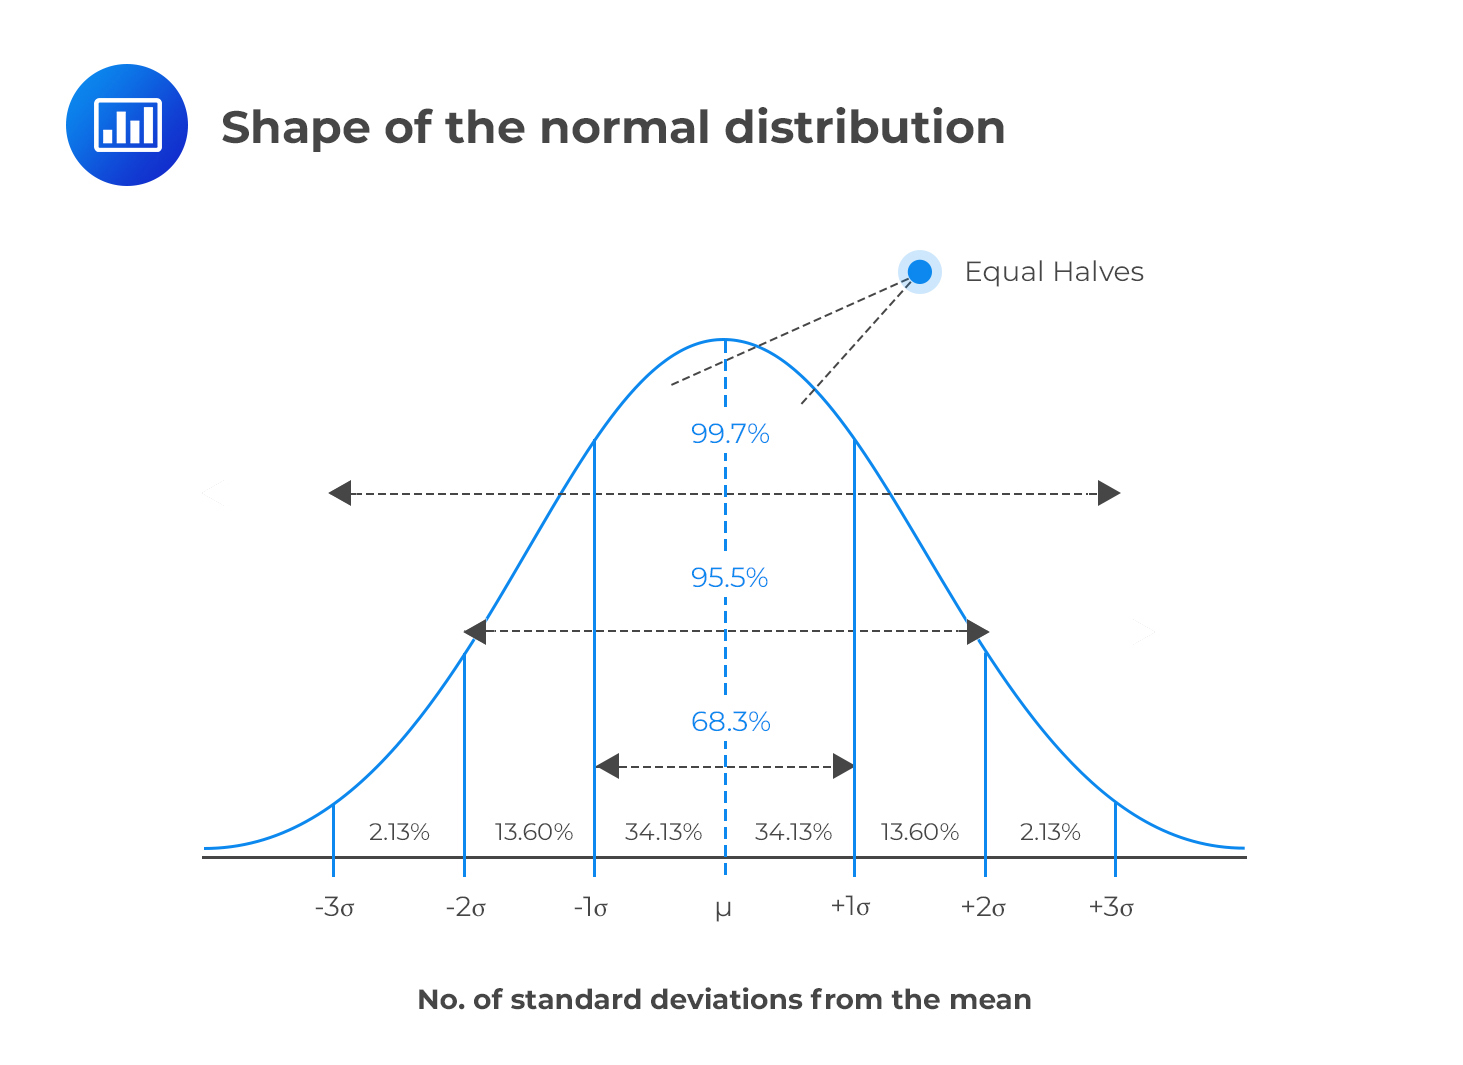
\includegraphics[width=20.32in]{images/normal}

The value of 1.96 come from the normal distribution, where 95\% of the population lies between +/- 1.96 standard deviations of the mean. If we did not already know this, we could use the \emph{qnorm()} function in R to calculate the value:

\begin{Shaded}
\begin{Highlighting}[]
\CommentTok{# Calculate the number of standard deviations that contains 0% to 97.5% of the data (100% - 2.5%). }
\CommentTok{# We can then say that 95% of the data lies between + or - the answer: }

\KeywordTok{qnorm}\NormalTok{(}\FloatTok{0.975}\NormalTok{)}
\end{Highlighting}
\end{Shaded}

\begin{verbatim}
## [1] 1.959964
\end{verbatim}

However, with smaller samples, since we are less confident about generalising to the population, we use the t-distribution to calculate that value. The shape of a t-distribution changes based on the sample size, so the smaller the sample size is, the wider the range that 95\% of values lie between. We can calculate the 95\% value for a particular sample size in R using the \emph{qt()} function:

\begin{Shaded}
\begin{Highlighting}[]
\CommentTok{# The qt function relates to t-distribution}

\KeywordTok{qt}\NormalTok{(}\FloatTok{0.975}\NormalTok{,}\DataTypeTok{df=}\DecValTok{20-1}\NormalTok{)}
\end{Highlighting}
\end{Shaded}

\begin{verbatim}
## [1] 2.093024
\end{verbatim}

\begin{Shaded}
\begin{Highlighting}[]
\CommentTok{# for qt, we need to specify the degress of freedom, which is sample size minus 1}
\end{Highlighting}
\end{Shaded}

We can see that when we have a sample size of 20, 95\% of values in our predicted population distribution will lie between + and - 2.0930241 standard deviations. Therefore, we can calculate more accurate confidence intervals using this value:

\begin{Shaded}
\begin{Highlighting}[]
\KeywordTok{mean}\NormalTok{(happiness) }\OperatorTok{-}\StringTok{ }\KeywordTok{qt}\NormalTok{(}\FloatTok{0.975}\NormalTok{,}\DataTypeTok{df=}\DecValTok{20-1}\NormalTok{) }\OperatorTok{*}\StringTok{ }\NormalTok{standardError }\CommentTok{# Lower confidence interval}
\end{Highlighting}
\end{Shaded}

\begin{verbatim}
## [1] 8.802803
\end{verbatim}

\begin{Shaded}
\begin{Highlighting}[]
\KeywordTok{mean}\NormalTok{(happiness) }\OperatorTok{+}\StringTok{ }\KeywordTok{qt}\NormalTok{(}\FloatTok{0.975}\NormalTok{,}\DataTypeTok{df=}\DecValTok{20-1}\NormalTok{) }\OperatorTok{*}\StringTok{ }\NormalTok{standardError }\CommentTok{# Upper confidence interval}
\end{Highlighting}
\end{Shaded}

\begin{verbatim}
## [1] 10.4361
\end{verbatim}

\textbf{This tells us:} if we were to take infinite number of similar samples, about 95\% of their confidence intervals would contain the population mean. Therefore, we think it is reasonable to estimate that the population mean is somewhere in this range.

\begin{quote}
Often people say that a 95\% confidence interval means that there is a 95\% chance that the population mean is between the lower and upper confidence interval. This is \textbf{not} an accurate statement, but it is often used as a shorthand to help people conceptualise what confidence intervals are.
\end{quote}

\hypertarget{we-can-also-make-confidence-intervals-of-differences-between-means}{%
\section{We can also make confidence intervals of differences between means}\label{we-can-also-make-confidence-intervals-of-differences-between-means}}

Often when we test hypotheses, we are testing the difference between two samples. For example, we might have 2 groups who have undergone different psychological interventions and want to know whether the difference we see our participant samples is likely to generalise to the population.

\begin{table}

\caption{\label{tab:unnamed-chunk-9}Some sample data for happiness score with participants divided into 2 groups}
\centering
\begin{tabular}[t]{r|r|r}
\hline
participant & intervention & happiness\\
\hline
1 & 1 & 11.126738\\
\hline
2 & 2 & 11.455096\\
\hline
3 & 1 & 9.448889\\
\hline
4 & 1 & 6.567100\\
\hline
5 & 2 & 11.080759\\
\hline
6 & 1 & 9.866935\\
\hline
7 & 1 & 11.066079\\
\hline
8 & 2 & 7.115263\\
\hline
9 & 1 & 8.478822\\
\hline
10 & 2 & 9.126518\\
\hline
11 & 1 & 11.077905\\
\hline
12 & 2 & 11.238149\\
\hline
13 & 2 & 6.796180\\
\hline
14 & 2 & 7.745382\\
\hline
15 & 1 & 9.542996\\
\hline
16 & 1 & 7.913203\\
\hline
17 & 1 & 9.601031\\
\hline
18 & 1 & 10.571534\\
\hline
19 & 2 & 9.679823\\
\hline
20 & 2 & 12.890654\\
\hline
\end{tabular}
\end{table}

Using the same approach as in the previous section, we can estimate a confidence interval based on the difference in means and the sample size:

\begin{Shaded}
\begin{Highlighting}[]
\CommentTok{# Calculate the number of standard deviations for 95% of the data }
\KeywordTok{qt}\NormalTok{(}\FloatTok{0.975}\NormalTok{,}\DataTypeTok{df=}\DecValTok{20-2}\NormalTok{) }\CommentTok{# since there are 2 intervention groups, degrees of freedom is now 20-2}
\end{Highlighting}
\end{Shaded}

\begin{verbatim}
## [1] 2.100922
\end{verbatim}

\begin{Shaded}
\begin{Highlighting}[]
\NormalTok{ group1 <-}\StringTok{ }\NormalTok{happinessSample }\OperatorTok\StringTok{ }\KeywordTok{filter}\NormalTok{(intervention }\OperatorTok{==}\DecValTok{1}\NormalTok{) }\OperatorTok\StringTok{ }\KeywordTok{summarise}\NormalTok{(}\DataTypeTok{mean =} \KeywordTok{mean}\NormalTok{(happiness), }\DataTypeTok{sd=} \KeywordTok{sd}\NormalTok{(happiness)) }
 
\NormalTok{  group2 <-}\StringTok{ }\NormalTok{happinessSample }\OperatorTok\StringTok{ }\KeywordTok{filter}\NormalTok{(intervention }\OperatorTok{==}\DecValTok{2}\NormalTok{) }\OperatorTok\StringTok{ }\KeywordTok{summarise}\NormalTok{(}\DataTypeTok{mean =} \KeywordTok{mean}\NormalTok{(happiness), }\DataTypeTok{sd=} \KeywordTok{sd}\NormalTok{(happiness)) }

\CommentTok{# calculate mean of difference}
\NormalTok{meanDifference <-}\StringTok{ }\NormalTok{group1}\OperatorTok{$}\NormalTok{mean }\OperatorTok{-}\StringTok{ }\NormalTok{group2}\OperatorTok{$}\NormalTok{mean}
\NormalTok{seDifference <-}\StringTok{ }\KeywordTok{sqrt}\NormalTok{(((group1}\OperatorTok{$}\NormalTok{sd}\OperatorTok{^}\DecValTok{2}\NormalTok{)}\OperatorTok{/}\DecValTok{19}\NormalTok{) }\OperatorTok{+}\StringTok{ }\NormalTok{((group2}\OperatorTok{$}\NormalTok{sd}\OperatorTok{^}\DecValTok{2}\NormalTok{)}\OperatorTok{/}\DecValTok{19}\NormalTok{))}


\CommentTok{# calculate 95% CI of this}
\NormalTok{meanDifference }\OperatorTok{-}\StringTok{ }\NormalTok{seDifference }\OperatorTok{*}\StringTok{ }\KeywordTok{qt}\NormalTok{(}\KeywordTok{c}\NormalTok{(}\FloatTok{0.975}\NormalTok{), }\DecValTok{20-2}\NormalTok{) }\CommentTok{# lower CI}
\end{Highlighting}
\end{Shaded}

\begin{verbatim}
## [1] -1.35913
\end{verbatim}

\begin{Shaded}
\begin{Highlighting}[]
\NormalTok{meanDifference }\OperatorTok{+}\StringTok{ }\NormalTok{seDifference }\OperatorTok{*}\StringTok{ }\KeywordTok{qt}\NormalTok{(}\KeywordTok{c}\NormalTok{(}\FloatTok{0.975}\NormalTok{), }\DecValTok{20-2}\NormalTok{) }\CommentTok{# upper CI}
\end{Highlighting}
\end{Shaded}

\begin{verbatim}
## [1] 1.135797
\end{verbatim}

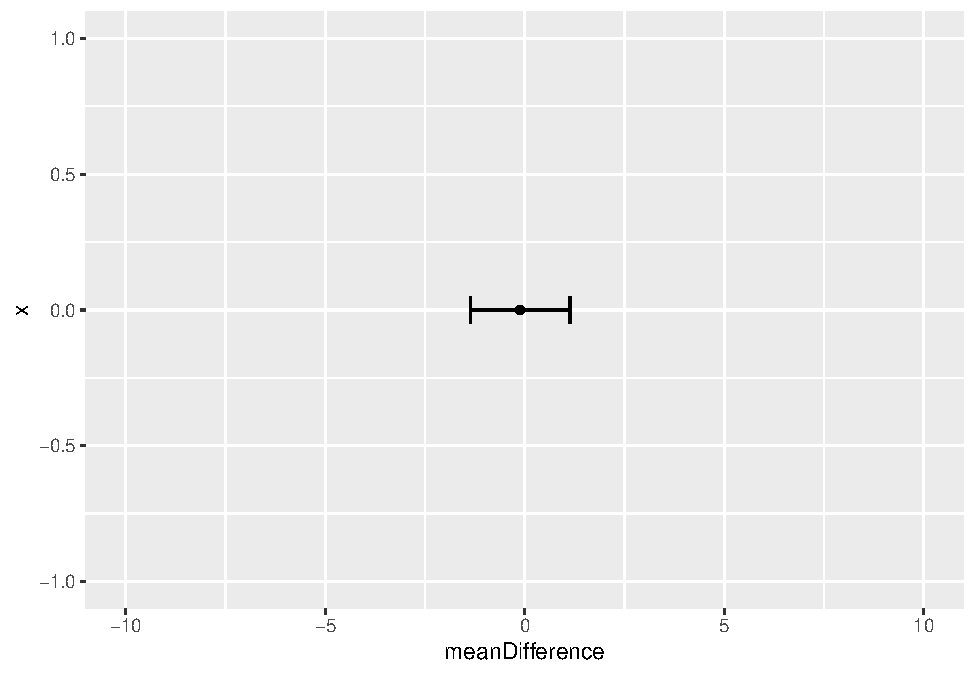
\includegraphics{PRBook_files/figure-latex/unnamed-chunk-11-1.pdf}

This tells use that the 95\% confidence interval of the difference is between -1.3591301 and 1.1357974. An important part of interpreting this, is to notice whether any point between these values is equal to zero. If the confidence interval of a difference contains a zero value, this means that in future research, with similar samples, it would be possible to see zero difference between the groups. If, on the other hand, the confidence interval does not cross zero, then it is likely that in future research, with similar samples, we would see some difference between the means.

\begin{quote}
The fact of whether confidence intervals cross zero (or not) is linked directly to the idea of hypothesis testing and statistical significance.
\end{quote}

\hypertarget{the-null-hypothesis-and-statistical-significance}{%
\section{The null hypothesis and statistical significance}\label{the-null-hypothesis-and-statistical-significance}}

Using the same study from the previous example: we know that the null hypothesis can be phrased as ``in the population, there is no difference between groups''. We then see how the confidence interval of a difference can help us test the null hypothesis: if the null hypothesis were not true, then it is unlikely that the confidence interval of the difference would contain zero.

Therefore, if confidence intervals overlap, then there is a possibility of no difference existing between the populations. As such, we are unable to reject the null hypothesis.

\hypertarget{introduction-to-r-and-r-studio}{%
\chapter{Introduction to R and R Studio}\label{introduction-to-r-and-r-studio}}

\hypertarget{by-the-end-of-this-section-you-should-be-able-to}{%
\section{By the end of this section, you should be able to:}\label{by-the-end-of-this-section-you-should-be-able-to}}

\begin{itemize}
\tightlist
\item
  Download R and R studio
\item
  Identify the R script, R console, Data environment and file browser in R studio
\item
  Write and run R code from a script
\item
  Install and load R packages
\end{itemize}

\hypertarget{why-learn-use-r}{%
\section{Why learn / use R?}\label{why-learn-use-r}}

\hypertarget{some-information-about-r}{%
\subsection{Some information about R}\label{some-information-about-r}}

\begin{itemize}
\tightlist
\item
  R is developed and used by scientists and researchers around the world
\item
  Open source = no cost
\item
  Constant development
\item
  Connects to other data science/research tools
\item
  Worldwide community: training widely available
\item
  Encourages transparency and reproducibility
\item
  Publication-ready outputs
\end{itemize}

\hypertarget{moving-from-other-software-to-r}{%
\subsection{Moving from other software to R}\label{moving-from-other-software-to-r}}

\begin{itemize}
\tightlist
\item
  Workflow is different

  \begin{itemize}
  \tightlist
  \item
    Organise files and data differently
  \item
    Workspace can contain data and outputs
  \item
    Can manage multiple datasets within a workspace
  \end{itemize}
\item
  Learning curve can be steep initially

  \begin{itemize}
  \tightlist
  \item
    e.g.~Variables and coding, scripts
  \end{itemize}
\item
  Need to know what you want

  \begin{itemize}
  \tightlist
  \item
    e.g.~building your regression model / ANOVA error terms
  \end{itemize}
\end{itemize}

\hypertarget{r-has-many-advantages}{%
\section{R has many advantages}\label{r-has-many-advantages}}

\begin{itemize}
\tightlist
\item
  Using scripts means analysis is easy to follow and reproduce
\item
  R scripts are small, online collaboration, no SPSS ``older version'' problems
\item
  Data can be organised and reorganised however you need it (tidyr)
\item
  Packages are available for ``cutting edge'' analysis: e.g.~Big Data \& Machine Learning
\item
  A robust language for precise plots and graphics (ggplot)
\item
  R analysis code can be embdeded into documents and presentations (R Markdown)
\end{itemize}

\hypertarget{download-r-and-r-studio}{%
\section{Download R and R Studio}\label{download-r-and-r-studio}}

Click on these links to download:

\begin{itemize}
\tightlist
\item
  \href{https://cran.r-project.org/}{R project}
\item
  \href{https://rstudio.com/}{RStudio}
\end{itemize}

\hypertarget{the-r-studio-environment}{%
\section{The R Studio environment}\label{the-r-studio-environment}}

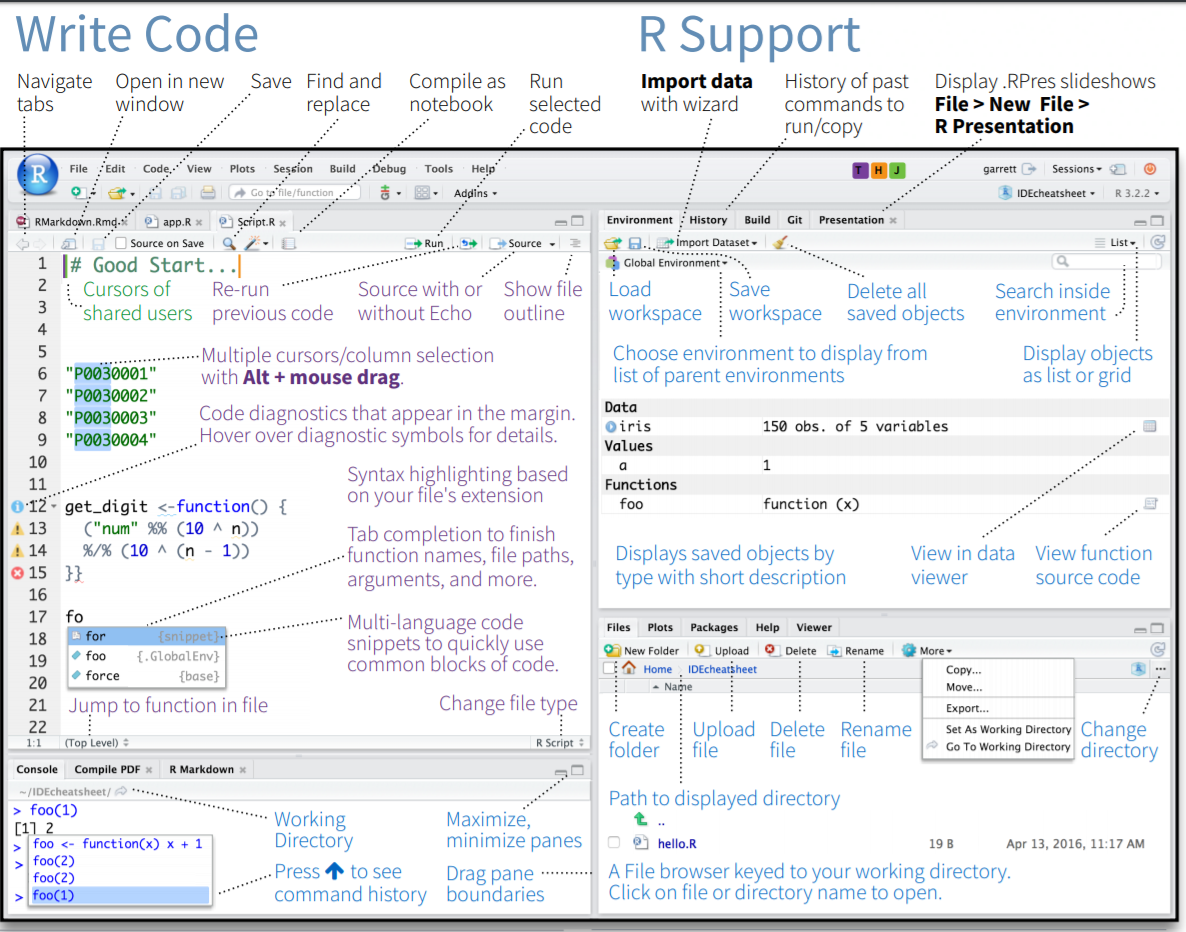
\includegraphics{images/rstudio_ide.png}
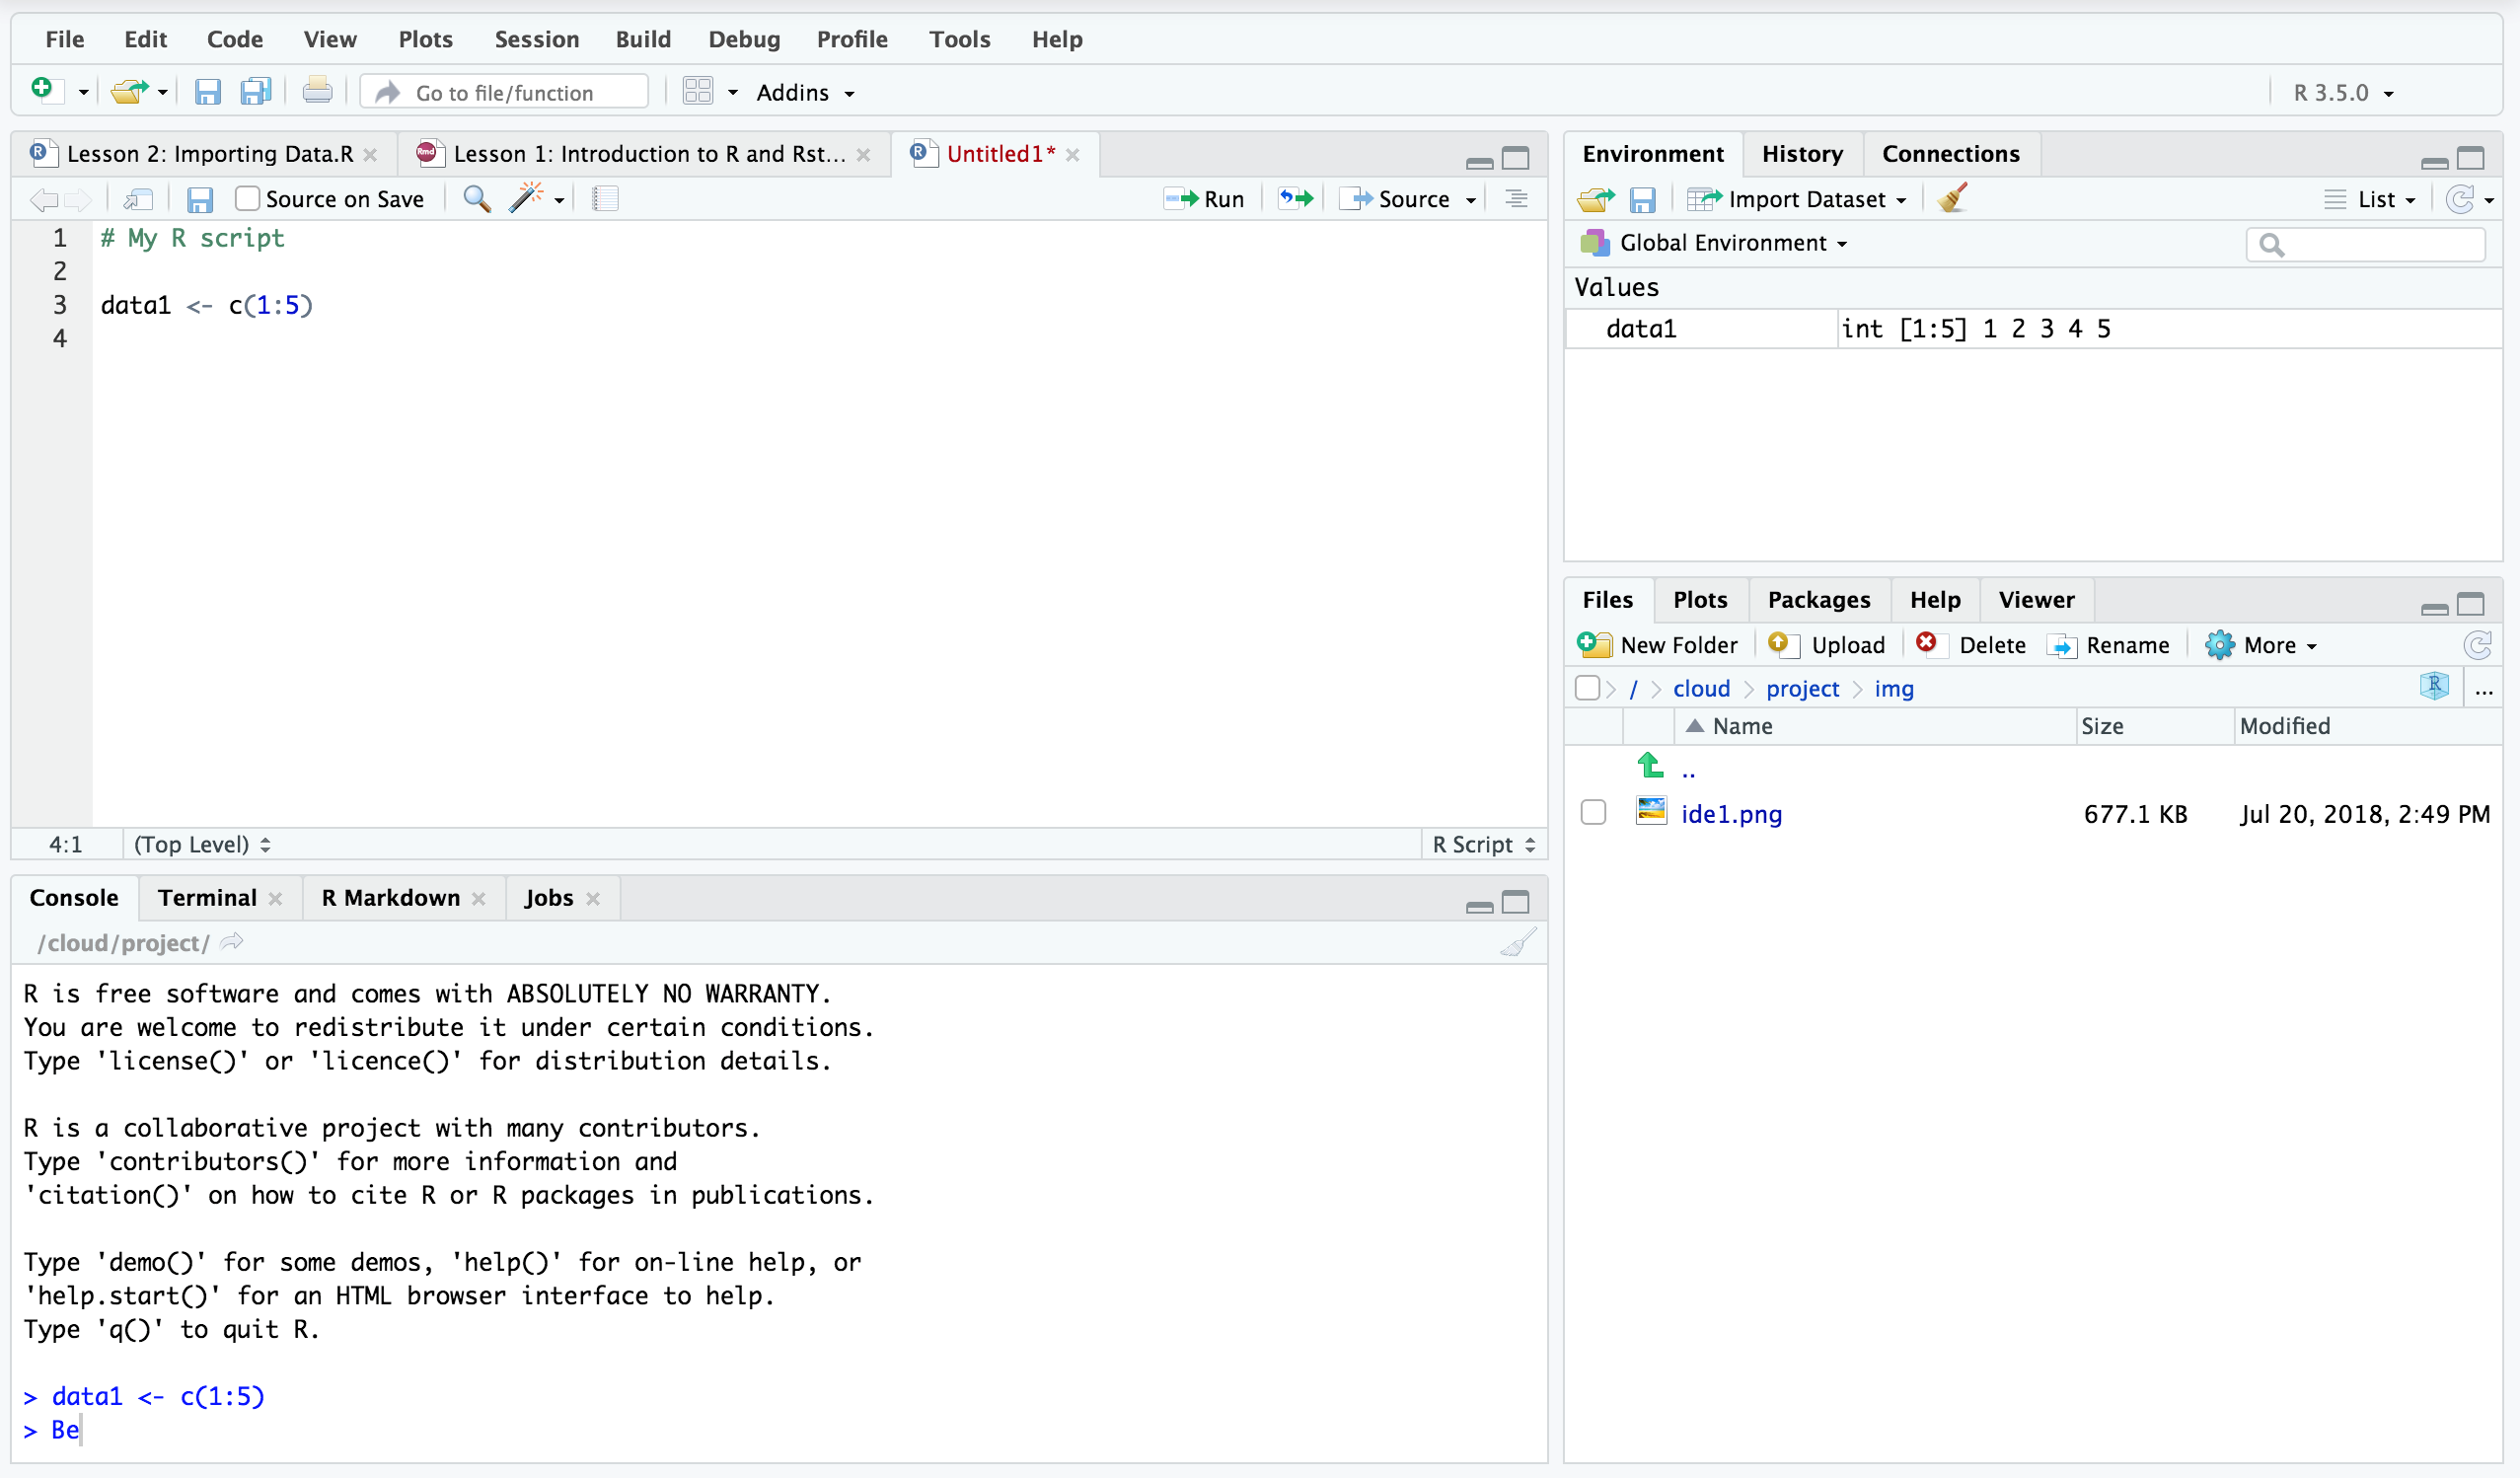
\includegraphics{images/rstudio1.png}

The interface for R Studio looks daunting at first. However, there are 4 main sections, 2 on the left and 2 on the right.

\begin{itemize}
\tightlist
\item
  MAIN TOP: R Script files or R Document Files

  \begin{itemize}
  \tightlist
  \item
    Where we usually type our code as a script before we run it. Script files are usually saved so we can work on them and rerun the code again later (.R files).
  \end{itemize}
\item
  MAIN BOTTOM: Console

  \begin{itemize}
  \tightlist
  \item
    Shows the output of our R code. We can type R code directly into the console and the answer will ouput immediately. However, it is more convenient to use script files.
  \end{itemize}
\item
  RIGHT TOP: Environment

  \begin{itemize}
  \tightlist
  \item
    Contains all of the objects (e.g.~data, analysis, equations, plots) that are currently stored in memory. We can save all of this to a file and load it later (.RData files).
  \end{itemize}
\item
  RIGHT BOTTOM: File Browser

  \begin{itemize}
  \tightlist
  \item
    The folder that R is working from is called `the working directory' and it will automatically look for files there if we try to import something (e.g.~a data file). Using the more button on the file browser allows you to set your desired working directory.
  \end{itemize}
\end{itemize}

\hypertarget{working-with-a-script}{%
\section{Working with a script}\label{working-with-a-script}}

Scripts can be opened from the \textbf{File} menu.

\begin{figure}
\centering
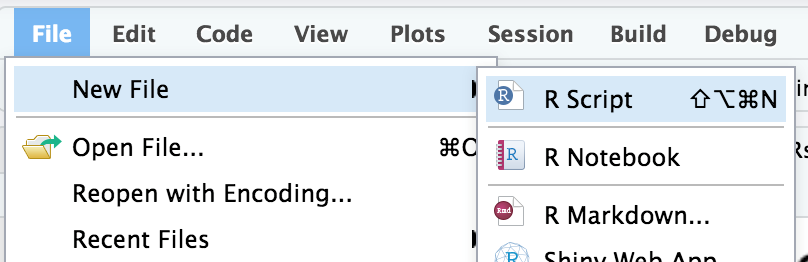
\includegraphics{images/file.png}
\caption{Creating a new script}
\end{figure}

The purpose of scripts is to allow you to type your analysis code and save it for use later. Scripts include, for example:

\begin{itemize}
\tightlist
\item
  Code for importing data into R
\item
  Your analysis code (e.g.~t-test or descriptive statistics)
\item
  Code for graphs and tables
\item
  Comments and notes (preceded by the `\#' symbol)
\end{itemize}

\begin{figure}
\centering
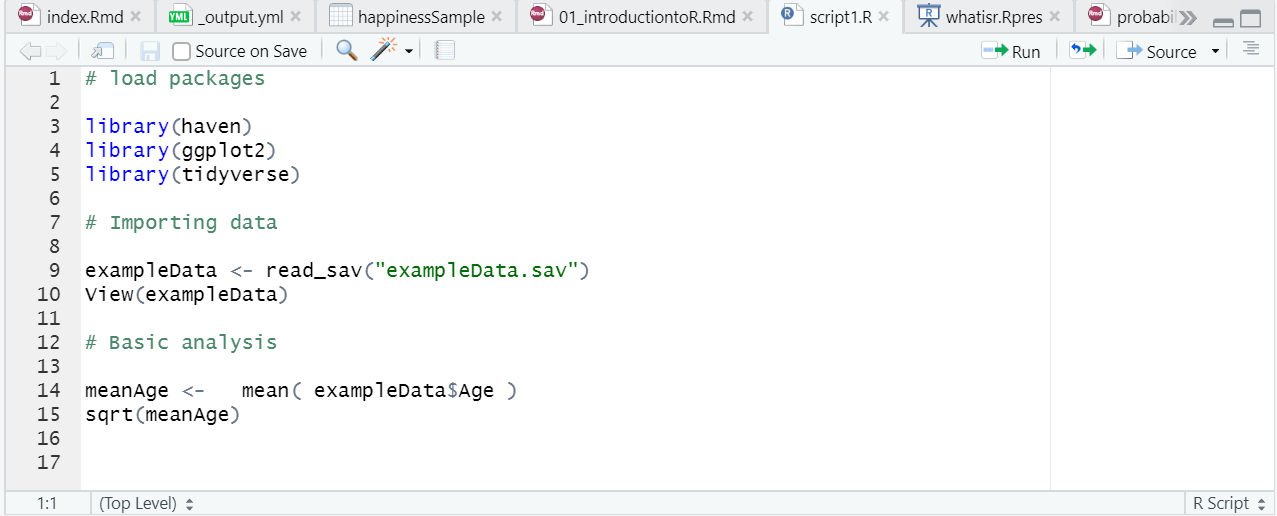
\includegraphics{images/script.png}
\caption{Example of an R script}
\end{figure}

To run a script, you click the \textbf{Run} button. You can choose to:

\begin{itemize}
\tightlist
\item
  Run the whole script
\item
  Run the selected line of code
\end{itemize}

\begin{figure}
\centering
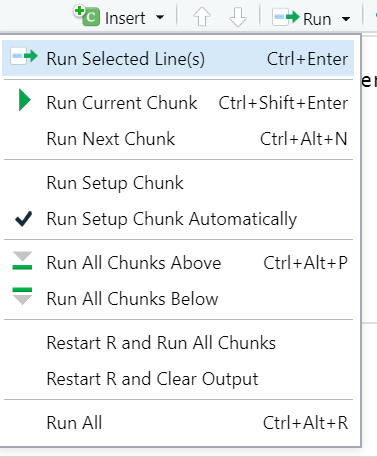
\includegraphics{images/run.png}
\caption{The run button}
\end{figure}

When you run the script, you will normally see output in the \textbf{console.}

\begin{figure}
\centering
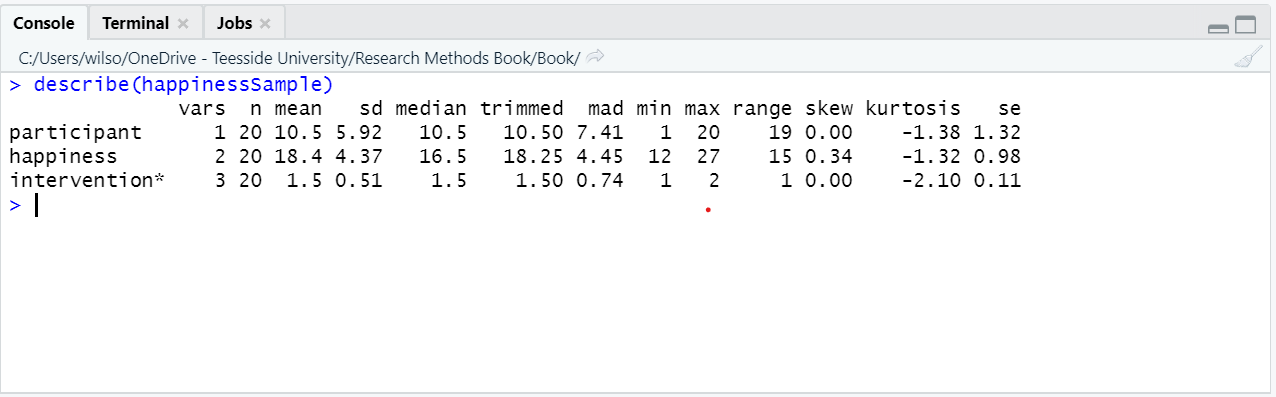
\includegraphics{images/console.png}
\caption{Output appears in the console}
\end{figure}

If your script contains code for a plot (graph), it will appear in the \textbf{Plots} window in the bottom right.

\begin{figure}
\centering
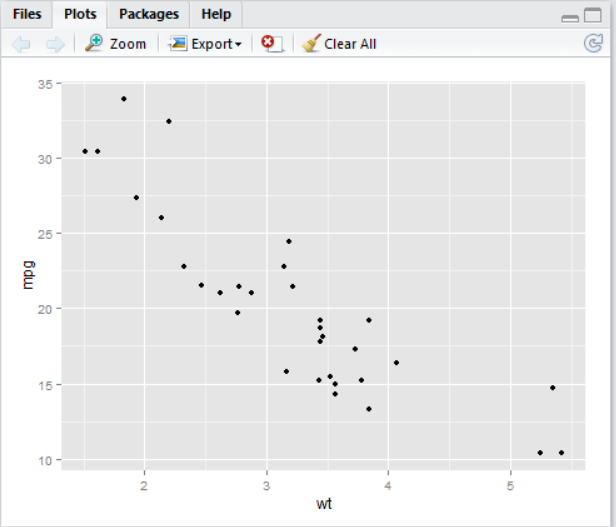
\includegraphics{images/plotwindow.png}
\caption{Plots appear in the plot window}
\end{figure}

\hypertarget{installing-and-loading-packages}{%
\section{Installing and loading packages}\label{installing-and-loading-packages}}

install Packages from RStudio, Inc. on Vimeo.

Packages add functionality to R and allow us to do new types of analysis.

\begin{itemize}
\item
  They can be installed via the menu (Tools -\textgreater{} Install Packages)
\item
  The can also be installed using code:

\begin{verbatim}
    install.packages()
\end{verbatim}
\end{itemize}

For example, TidyR is a package that contains functions for sorting and organising data. To install the package:

\begin{figure}
\centering
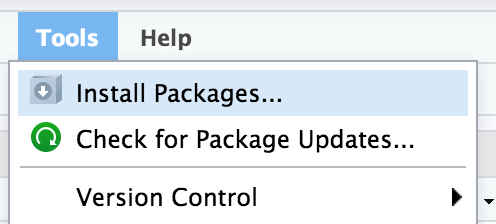
\includegraphics{images/installPackages.png}
\caption{Installing a package in RStudio}
\end{figure}

or use the code:

\begin{verbatim}
install.packages(“tidyr”)
\end{verbatim}

Once a package is has been installed, you need tp load it using the \emph{library()} command.
For example:

\begin{verbatim}
library(“tidyr”)
\end{verbatim}

\hypertarget{working-with-data-in-r}{%
\chapter{Working with data in R}\label{working-with-data-in-r}}

\hypertarget{by-the-end-of-this-section-you-will-be-able-to}{%
\section{By the end of this section, you will be able to:}\label{by-the-end-of-this-section-you-will-be-able-to}}

\begin{itemize}
\tightlist
\item
  Import data into R from excel, SPSS and csv files
\item
  Save data to objects
\item
  Identify different data structures and variable types
\item
  Convert variables from one type to another
\item
  Order, filter and group data
\item
  Summarise data
\item
  Create new variables from data
\end{itemize}

\hypertarget{in-this-section-we-will-use-the-tidyverse-set-of-packages}{%
\section{In this section, we will use the Tidyverse set of packages}\label{in-this-section-we-will-use-the-tidyverse-set-of-packages}}

\begin{itemize}
\tightlist
\item
  A `toolkit' of packages that are very useful for organsing and manipulating data
\item
  We will use the haven package to import SPSS files
\item
  We will use the dplyr to organise data
\item
  Also includes the ggplot2 and tidyR packages which we will use later
\end{itemize}

To install:

\begin{verbatim}
install.packages(“tidyverse”)
\end{verbatim}

(See the previous section on installing packages)

\hypertarget{import-data-into-r-from-excel-spss-and-csv-files}{%
\section{Import data into R from excel, SPSS and csv files}\label{import-data-into-r-from-excel-spss-and-csv-files}}

We can import data from a range of sources using the \textbf{Import Dataset} button in the \textbf{Environment} tab:

\begin{figure}
\centering
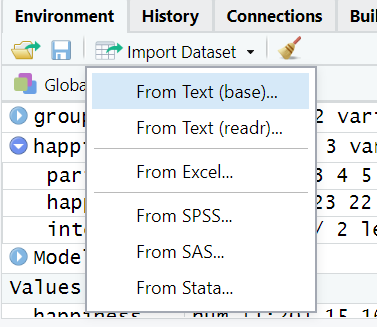
\includegraphics{images/importData.png}
\caption{Importing data}
\end{figure}

It is also possible to import data using code, for example:

\begin{verbatim}
# importing a .csv file
library(readr)
studentData <- read_csv("Datasets/studentData.csv")


#importing an SPSS file
library(haven)
mySPSSData <- read_sav("Datasets/salesData.sav")
\end{verbatim}

Once the data are imported, it will be visible in the environment:

\begin{figure}
\centering
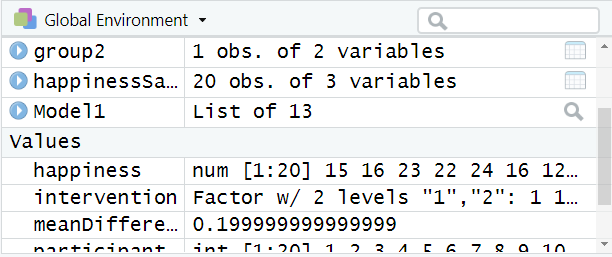
\includegraphics{images/environment.png}
\caption{Imported data in the environment}
\end{figure}

\hypertarget{understanding-objects-in-r}{%
\section{Understanding objects in R}\label{understanding-objects-in-r}}

In R, an \textbf{object} is anything that is saved to memory. For example, we might do some analysis:

\begin{verbatim}
mean(happiness)
\end{verbatim}

However, in the example above, the result would appear in the console but not be saved anywhere. To store the result for reuse later, we save it to an object:

\begin{verbatim}
happinessMean <- mean(happiness)
\end{verbatim}

In the above code (reading left to right):

\begin{itemize}
\tightlist
\item
  We name the object ``happinessMean''. This name can be anything we want.
\item
  The arrow means that the result of the code on the right will be saved to the object on the left.
\item
  The code on the right of the arrow calculates the mean of \emph{happiness} data
\end{itemize}

When this code is run, \emph{happinessMean} will be stored in the environment window:

\begin{figure}
\centering
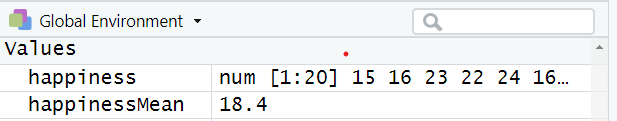
\includegraphics{images/saveobject.png}
\caption{Result of a calculation in the environment}
\end{figure}

To recall an object from the environment, we can simply type its name. For example:

\begin{verbatim}
happinessMean 
\end{verbatim}

\begin{quote}
Its important to note that anything can be stored as an object in R and recalled later. This includes, dataframes, the results of statistical calculations, plots etc.
\end{quote}

\hypertarget{identify-different-data-structures-and-variable-types}{%
\section{Identify different data structures and variable types}\label{identify-different-data-structures-and-variable-types}}

\hypertarget{data-structures}{%
\subsection{Data structures}\label{data-structures}}

There are many different types of data that R can work with. The most common type of data for most people tends to be a \textbf{dataframe}. A \textbf{dataframe} is what you might consider a ``normal'' 2-dimensional dataset, with rows of data and columns of variables:

\begin{figure}
\centering
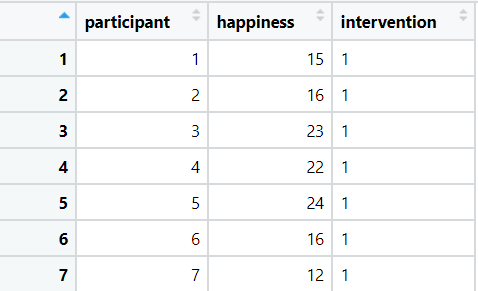
\includegraphics{images/dataframe.png}
\caption{A dataframe example}
\end{figure}

R can also use other data types.

A vector is a one-dimensional set of values:

\begin{Shaded}
\begin{Highlighting}[]
\CommentTok{# a vector example}

\NormalTok{scores <-}\StringTok{ }\KeywordTok{c}\NormalTok{(}\DecValTok{1}\NormalTok{,}\DecValTok{4}\NormalTok{,}\DecValTok{6}\NormalTok{,}\DecValTok{8}\NormalTok{,}\DecValTok{3}\NormalTok{,}\DecValTok{4}\NormalTok{,}\DecValTok{6}\NormalTok{,}\DecValTok{7}\NormalTok{)}
\end{Highlighting}
\end{Shaded}

A matrix is a multi-dimensional set of values. The below example is a 3-dimensional matrix, there are 2 groups of 2 rows and 3 columns:

\begin{verbatim}
## , , 1
## 
##      [,1] [,2] [,3]
## [1,]    1    3    5
## [2,]    2    4    6
## 
## , , 2
## 
##      [,1] [,2] [,3]
## [1,]    7    9   11
## [2,]    8   10   12
\end{verbatim}

\begin{quote}
We will primarily work with dataframes (and sometimes vectors), as this is how the data in psychology research is usually structured.
\end{quote}

\hypertarget{variable-types}{%
\subsection{Variable types}\label{variable-types}}

With numerical data, there are 4 key data types:

\begin{itemize}
\tightlist
\item
  Nominal (a category, group or factor)
\item
  Ordinal (a ranking)
\item
  Interval (scale data that can include negative values)
\item
  Ratio (scale data that cannot include negative values)
\end{itemize}

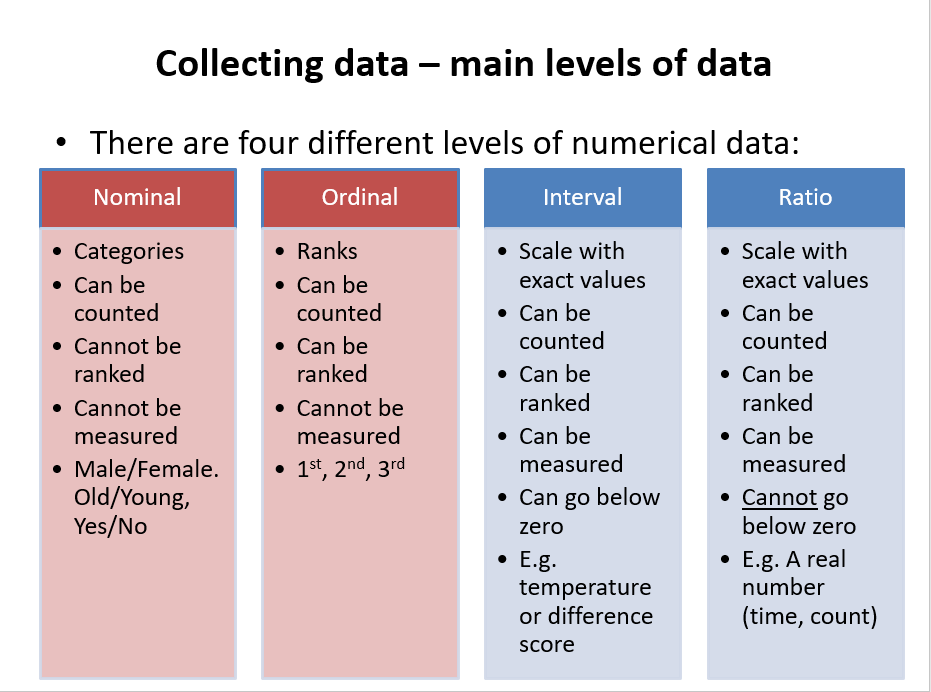
\includegraphics{images/dataTypes.png}
R can use all of these variable types:

\begin{itemize}
\tightlist
\item
  \textbf{Nominal} variables are called \textbf{factors}
\item
  \textbf{Ordinal} variables are called \textbf{ordered factors}
\item
  \textbf{Interval and ratio} variables are called \textbf{numeric} data and can sometimes be called integers (if they are only whole numbers) or doubles (if they all have decimal points)
\end{itemize}

R can also use other data types such as text (\textbf{character}) data.

\hypertarget{convert-variables-from-one-type-to-another}{%
\subsection{Convert variables from one type to another}\label{convert-variables-from-one-type-to-another}}

When we first import data into R, it might not recognise the data types correctly. For example, in the below data, we can see the \textbf{intervention} variable :

\begin{verbatim}
##    participant intervention happiness
## 1            4            1  6.567100
## 2           13            2  6.796180
## 3            8            2  7.115263
## 4           14            2  7.745382
## 5           16            1  7.913203
## 6            9            1  8.478822
## 7           10            2  9.126518
## 8            3            1  9.448889
## 9           15            1  9.542996
## 10          17            1  9.601031
\end{verbatim}

In the \textbf{intervention} variable, the numbers 1 and 2 refer to different intervention groups. Therefore, the variable is a \textbf{factor} variable. To ensure that R understands this, we can resave the intervention variable as a factor using the \emph{as.factor()} function:

\begin{Shaded}
\begin{Highlighting}[]
\NormalTok{happinessSample}\OperatorTok{$}\NormalTok{intervention <-}\StringTok{ }\KeywordTok{as.factor}\NormalTok{(happinessSample}\OperatorTok{$}\NormalTok{intervention)}
\end{Highlighting}
\end{Shaded}

\hypertarget{working-with-dataframes}{%
\section{Working with dataframes}\label{working-with-dataframes}}

Dataframes are the more standard data format that were are used to (think of how a dataset looks in SPSS or Excel).

In a dataframe, variables are columns and each row usually reperesents one measurement or one participant.

\hypertarget{view-dataframe}{%
\subsection{View dataframe}\label{view-dataframe}}

To view a dataframe, we can click on it in the environment window and it will display:

\begin{figure}
\centering
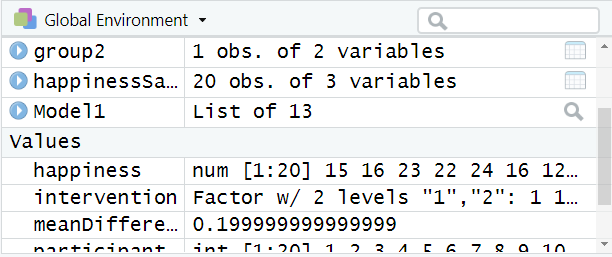
\includegraphics{images/environment.png}
\caption{Clicking on datasets in hte environment will open them up for viewing}
\end{figure}

\begin{figure}
\centering
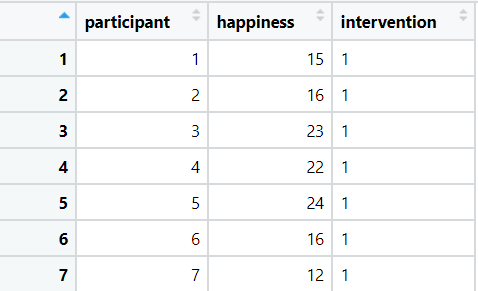
\includegraphics{images/dataframe.png}
\caption{Viewing a dataframe}
\end{figure}

\hypertarget{refer-to-variables-columns-in-a-dataframe}{%
\subsection{Refer to variables (columns) in a dataframe}\label{refer-to-variables-columns-in-a-dataframe}}

Columns in a dataframe are accessed using the ``\$'' sign. For example, to access the \emph{happiness} column in the \emph{happinessSample} dataframe, we would type:

\begin{Shaded}
\begin{Highlighting}[]
\NormalTok{happinessSample}\OperatorTok{$}\NormalTok{happiness}
\end{Highlighting}
\end{Shaded}

\begin{verbatim}
##  [1] 11.126738 11.455096  9.448889  6.567100 11.080759  9.866935 11.066079
##  [8]  7.115263  8.478822  9.126518 11.077905 11.238149  6.796180  7.745382
## [15]  9.542996  7.913203  9.601031 10.571534  9.679823 12.890654
\end{verbatim}

As we can see above, the result is then displayed.

\hypertarget{order-filter-and-group-data}{%
\section{Order, filter and group data}\label{order-filter-and-group-data}}

If you have the \textbf{tidyverse} package loaded, it is easy to organise and filter data.

\begin{Shaded}
\begin{Highlighting}[]
\KeywordTok{arrange}\NormalTok{(happinessSample, happiness)}
\end{Highlighting}
\end{Shaded}

\begin{verbatim}
##    participant intervention happiness
## 1            4            1  6.567100
## 2           13            2  6.796180
## 3            8            2  7.115263
## 4           14            2  7.745382
## 5           16            1  7.913203
## 6            9            1  8.478822
## 7           10            2  9.126518
## 8            3            1  9.448889
## 9           15            1  9.542996
## 10          17            1  9.601031
## 11          19            2  9.679823
## 12           6            1  9.866935
## 13          18            1 10.571534
## 14           7            1 11.066079
## 15          11            1 11.077905
## 16           5            2 11.080759
## 17           1            1 11.126738
## 18          12            2 11.238149
## 19           2            2 11.455096
## 20          20            2 12.890654
\end{verbatim}

\begin{Shaded}
\begin{Highlighting}[]
\KeywordTok{arrange}\NormalTok{(happinessSample, }\KeywordTok{desc}\NormalTok{(happiness)) }\CommentTok{# Arrange in descending order}
\end{Highlighting}
\end{Shaded}

\begin{verbatim}
##    participant intervention happiness
## 1           20            2 12.890654
## 2            2            2 11.455096
## 3           12            2 11.238149
## 4            1            1 11.126738
## 5            5            2 11.080759
## 6           11            1 11.077905
## 7            7            1 11.066079
## 8           18            1 10.571534
## 9            6            1  9.866935
## 10          19            2  9.679823
## 11          17            1  9.601031
## 12          15            1  9.542996
## 13           3            1  9.448889
## 14          10            2  9.126518
## 15           9            1  8.478822
## 16          16            1  7.913203
## 17          14            2  7.745382
## 18           8            2  7.115263
## 19          13            2  6.796180
## 20           4            1  6.567100
\end{verbatim}

\begin{itemize}
\tightlist
\item
  Show clients with a happiness score of less than 4
\end{itemize}

\begin{Shaded}
\begin{Highlighting}[]
\KeywordTok{filter}\NormalTok{(happinessSample, happiness }\OperatorTok{<}\StringTok{ }\DecValTok{4}\NormalTok{)}
\end{Highlighting}
\end{Shaded}

\begin{verbatim}
## [1] participant  intervention happiness   
## <0 rows> (or 0-length row.names)
\end{verbatim}

\begin{itemize}
\tightlist
\item
  Show Intervention group 2 with happiness scores above 7
\end{itemize}

\begin{Shaded}
\begin{Highlighting}[]
\KeywordTok{filter}\NormalTok{(happinessSample, happiness }\OperatorTok{>}\StringTok{ }\DecValTok{7} \OperatorTok{&}\StringTok{ }\NormalTok{intervention }\OperatorTok{==}\StringTok{ }\DecValTok{2}\NormalTok{)}
\end{Highlighting}
\end{Shaded}

\begin{verbatim}
##   participant intervention happiness
## 1           2            2 11.455096
## 2           5            2 11.080759
## 3           8            2  7.115263
## 4          10            2  9.126518
## 5          12            2 11.238149
## 6          14            2  7.745382
## 7          19            2  9.679823
## 8          20            2 12.890654
\end{verbatim}

\begin{itemize}
\tightlist
\item
  Group by intervention and show the mean happiness score
\end{itemize}

\begin{Shaded}
\begin{Highlighting}[]
\NormalTok{happinessSample }\OperatorTok\StringTok{ }\KeywordTok{group_by}\NormalTok{(intervention) }\OperatorTok\StringTok{ }\KeywordTok{summarise}\NormalTok{(}\DataTypeTok{mean =} \KeywordTok{mean}\NormalTok{(happiness))}
\end{Highlighting}
\end{Shaded}

\begin{verbatim}
## `summarise()` ungrouping output (override with `.groups` argument)
\end{verbatim}

\begin{verbatim}
## # A tibble: 2 x 2
##   intervention  mean
##   <fct>        <dbl>
## 1 1             9.57
## 2 2             9.68
\end{verbatim}

\hypertarget{create-new-variables-from-data}{%
\section{Create new variables from data}\label{create-new-variables-from-data}}

To create new variables from data, we can use the \textbf{mutate()} function.

For example, let's say we wanted to calculate the difference between each person's happiness score and the mean happiness score.

We could do the following:

\begin{Shaded}
\begin{Highlighting}[]
\NormalTok{happinessSample }\OperatorTok\StringTok{ }\KeywordTok{mutate}\NormalTok{(}\DataTypeTok{difference =}\NormalTok{ happiness }\OperatorTok{-}\StringTok{ }\KeywordTok{mean}\NormalTok{(happiness))}
\end{Highlighting}
\end{Shaded}

\begin{verbatim}
##    participant intervention happiness  difference
## 1            1            1 11.126738  1.50728529
## 2            2            2 11.455096  1.83564318
## 3            3            1  9.448889 -0.17056384
## 4            4            1  6.567100 -3.05235257
## 5            5            2 11.080759  1.46130629
## 6            6            1  9.866935  0.24748237
## 7            7            1 11.066079  1.44662657
## 8            8            2  7.115263 -2.50418981
## 9            9            1  8.478822 -1.14063086
## 10          10            2  9.126518 -0.49293472
## 11          11            1 11.077905  1.45845198
## 12          12            2 11.238149  1.61869598
## 13          13            2  6.796180 -2.82327322
## 14          14            2  7.745382 -1.87407077
## 15          15            1  9.542996 -0.07645695
## 16          16            1  7.913203 -1.70624991
## 17          17            1  9.601031 -0.01842209
## 18          18            1 10.571534  0.95208145
## 19          19            2  9.679823  0.06037042
## 20          20            2 12.890654  3.27120122
\end{verbatim}

\hypertarget{exploratory-and-descriptive-analysis-with-r}{%
\chapter{Exploratory and descriptive analysis with R}\label{exploratory-and-descriptive-analysis-with-r}}

\hypertarget{working-example---record-sales-data}{%
\section{Working example - record sales data}\label{working-example---record-sales-data}}

Let's import the data \{.smaller\}

\begin{Shaded}
\begin{Highlighting}[]
\NormalTok{Album_Sales <-}\StringTok{ }\KeywordTok{read_csv}\NormalTok{(}\StringTok{"Datasets/album_sales.csv"}\NormalTok{)}
\end{Highlighting}
\end{Shaded}

\begin{verbatim}
## Parsed with column specification:
## cols(
##   Adverts = col_double(),
##   Sales = col_double(),
##   Airplay = col_double(),
##   Attract = col_double(),
##   Genre = col_character()
## )
\end{verbatim}

Let's look at the data \{.smaller\}

\begin{Shaded}
\begin{Highlighting}[]
\KeywordTok{head}\NormalTok{(Album_Sales)}
\end{Highlighting}
\end{Shaded}

\begin{verbatim}
## # A tibble: 6 x 5
##   Adverts Sales Airplay Attract Genre  
##     <dbl> <dbl>   <dbl>   <dbl> <chr>  
## 1    10.3   330      43      10 Country
## 2   986.    120      28       7 Pop    
## 3  1446.    360      35       7 HipHop 
## 4  1188.    270      33       7 HipHop 
## 5   575.    220      44       5 Metal  
## 6   569.    170      19       5 Country
\end{verbatim}

\hypertarget{lets-make-sure-our-data-types-are-correct-1}{%
\section{Let's make sure our data types are correct \#1}\label{lets-make-sure-our-data-types-are-correct-1}}

\begin{itemize}
\tightlist
\item
  This variable is currently stored as charcters, not as a factor / category variable
\end{itemize}

\begin{Shaded}
\begin{Highlighting}[]
\KeywordTok{str}\NormalTok{(Album_Sales}\OperatorTok{$}\NormalTok{Genre) }
\end{Highlighting}
\end{Shaded}

\begin{verbatim}
##  chr [1:200] "Country" "Pop" "HipHop" "HipHop" "Metal" "Country" "Pop" ...
\end{verbatim}

\begin{itemize}
\tightlist
\item
  We can save it as a factor
\end{itemize}

\begin{Shaded}
\begin{Highlighting}[]
\NormalTok{Album_Sales}\OperatorTok{$}\NormalTok{Genre <-}\StringTok{ }\KeywordTok{as.factor}\NormalTok{(Album_Sales}\OperatorTok{$}\NormalTok{Genre)}

\KeywordTok{str}\NormalTok{(Album_Sales}\OperatorTok{$}\NormalTok{Genre) }
\end{Highlighting}
\end{Shaded}

\begin{verbatim}
##  Factor w/ 4 levels "Country","HipHop",..: 1 4 2 2 3 1 4 4 3 2 ...
\end{verbatim}

\hypertarget{measures-of-central-tendency}{%
\section{Measures of central tendency}\label{measures-of-central-tendency}}

The main measures of central tendency are:
- Mean
- Median
- Mode

\hypertarget{mean}{%
\subsection{Mean}\label{mean}}

``What is the mean of album sales?''

\begin{Shaded}
\begin{Highlighting}[]
\KeywordTok{mean}\NormalTok{(Album_Sales}\OperatorTok{$}\NormalTok{Sales)}
\end{Highlighting}
\end{Shaded}

\begin{verbatim}
## [1] 193.2
\end{verbatim}

\hypertarget{trimmed-mean}{%
\subsection{Trimmed mean}\label{trimmed-mean}}

\begin{itemize}
\tightlist
\item
  The trimmed mean is used to reduce the influence of outliers on the summary
\end{itemize}

\begin{Shaded}
\begin{Highlighting}[]
\KeywordTok{mean}\NormalTok{(Album_Sales}\OperatorTok{$}\NormalTok{Sales, }\DataTypeTok{trim =} \FloatTok{0.05}\NormalTok{)}
\end{Highlighting}
\end{Shaded}

\begin{verbatim}
## [1] 192.6667
\end{verbatim}

\hypertarget{median}{%
\subsection{Median}\label{median}}

``What is the median amount of Airplay?''

\begin{Shaded}
\begin{Highlighting}[]
\KeywordTok{median}\NormalTok{(Album_Sales}\OperatorTok{$}\NormalTok{Airplay)}
\end{Highlighting}
\end{Shaded}

\begin{verbatim}
## [1] 28
\end{verbatim}

\hypertarget{mode}{%
\subsection{Mode}\label{mode}}

``What is the most common attractiveness rating of bands?''

\begin{itemize}
\tightlist
\item
  The easiest way to get the mode in R is to generate a frequency table
\end{itemize}

\begin{Shaded}
\begin{Highlighting}[]
\KeywordTok{table}\NormalTok{(Album_Sales}\OperatorTok{$}\NormalTok{Attract)}
\end{Highlighting}
\end{Shaded}

\begin{verbatim}
## 
##  1  2  3  4  5  6  7  8  9 10 
##  3  1  1  4 17 44 73 44 12  1
\end{verbatim}

\begin{itemize}
\tightlist
\item
  We can then look for the most frequently occuring response
\end{itemize}

\hypertarget{measures-of-dispresion-or-variance}{%
\section{Measures of dispresion or variance}\label{measures-of-dispresion-or-variance}}

\hypertarget{range}{%
\subsection{Range}\label{range}}

The range is the difference between the lowest and highest values

\begin{itemize}
\tightlist
\item
  You can calculate it using these values
\end{itemize}

\begin{Shaded}
\begin{Highlighting}[]
\KeywordTok{max}\NormalTok{(Album_Sales}\OperatorTok{$}\NormalTok{Airplay) }\OperatorTok{-}\StringTok{ }\KeywordTok{min}\NormalTok{(Album_Sales}\OperatorTok{$}\NormalTok{Airplay)}
\end{Highlighting}
\end{Shaded}

\begin{verbatim}
## [1] 63
\end{verbatim}

\begin{itemize}
\tightlist
\item
  Or you can use the range command to get the min and max values in one go
\end{itemize}

\begin{Shaded}
\begin{Highlighting}[]
\KeywordTok{range}\NormalTok{(Album_Sales}\OperatorTok{$}\NormalTok{Airplay)}
\end{Highlighting}
\end{Shaded}

\begin{verbatim}
## [1]  0 63
\end{verbatim}

\hypertarget{interquartile-range}{%
\subsection{Interquartile range}\label{interquartile-range}}

\begin{itemize}
\tightlist
\item
  We know that the median is the ``middle'' of the data = 50th percentile
\item
  The interquatile range is the difference between the values at the 25th and 75th percentiles
\end{itemize}

\begin{Shaded}
\begin{Highlighting}[]
\KeywordTok{quantile}\NormalTok{( }\DataTypeTok{x =}\NormalTok{ Album_Sales}\OperatorTok{$}\NormalTok{Airplay, }\DataTypeTok{probs =} \KeywordTok{c}\NormalTok{(.}\DecValTok{25}\NormalTok{,.}\DecValTok{75}\NormalTok{) )}
\end{Highlighting}
\end{Shaded}

\begin{verbatim}
##   25%   75% 
## 19.75 36.00
\end{verbatim}

\begin{itemize}
\tightlist
\item
  Interquartile range = 36 - 19.75 = 16.25
\end{itemize}

Sum of squares \{.smaller\}

\begin{itemize}
\tightlist
\item
  The difference between each value and the mean value, squared, and then summed together
\end{itemize}

\begin{Shaded}
\begin{Highlighting}[]
\KeywordTok{sum}\NormalTok{( (Album_Sales}\OperatorTok{$}\NormalTok{Adverts }\OperatorTok{-}\StringTok{ }\KeywordTok{mean}\NormalTok{(Album_Sales}\OperatorTok{$}\NormalTok{Adverts))}\OperatorTok{^}\DecValTok{2}\NormalTok{ )}
\end{Highlighting}
\end{Shaded}

\begin{verbatim}
## [1] 46936335
\end{verbatim}

\hypertarget{variance}{%
\subsection{Variance}\label{variance}}

\begin{itemize}
\tightlist
\item
  Variance: Sum of sqaures divided by n-1
\end{itemize}

\begin{Shaded}
\begin{Highlighting}[]
\CommentTok{# variance calculation}
\NormalTok{varianceAdverts <-}\StringTok{ }\KeywordTok{sum}\NormalTok{( (Album_Sales}\OperatorTok{$}\NormalTok{Adverts }\OperatorTok{-}\StringTok{ }\KeywordTok{mean}\NormalTok{(Album_Sales}\OperatorTok{$}\NormalTok{Adverts))}\OperatorTok{^}\DecValTok{2}\NormalTok{ ) }\OperatorTok{/}\StringTok{ }\DecValTok{199}
\end{Highlighting}
\end{Shaded}

\hypertarget{standard-deviation}{%
\subsection{Standard deviation}\label{standard-deviation}}

\begin{itemize}
\tightlist
\item
  Standard deviation is square root of the variance
\end{itemize}

\begin{Shaded}
\begin{Highlighting}[]
\CommentTok{# sd calculation}


\KeywordTok{sqrt}\NormalTok{(varianceAdverts)}
\end{Highlighting}
\end{Shaded}

\begin{verbatim}
## [1] 485.6552
\end{verbatim}

\begin{itemize}
\tightlist
\item
  Can be calculated using the sd() command
\end{itemize}

\begin{Shaded}
\begin{Highlighting}[]
\KeywordTok{sd}\NormalTok{(Album_Sales}\OperatorTok{$}\NormalTok{Adverts)}
\end{Highlighting}
\end{Shaded}

\begin{verbatim}
## [1] 485.6552
\end{verbatim}

\hypertarget{skewness-and-kurtosis}{%
\section{Skewness and Kurtosis}\label{skewness-and-kurtosis}}

\hypertarget{assessing-skewness-of-distribution-1}{%
\subsection{Assessing skewness of distribution \#1}\label{assessing-skewness-of-distribution-1}}

\begin{itemize}
\tightlist
\item
  It is possible to use graphs to view the distribution
\item
  We will focus on graphic presentation of data next week
\end{itemize}

\begin{Shaded}
\begin{Highlighting}[]
\KeywordTok{hist}\NormalTok{(Album_Sales}\OperatorTok{$}\NormalTok{Sales)}
\end{Highlighting}
\end{Shaded}

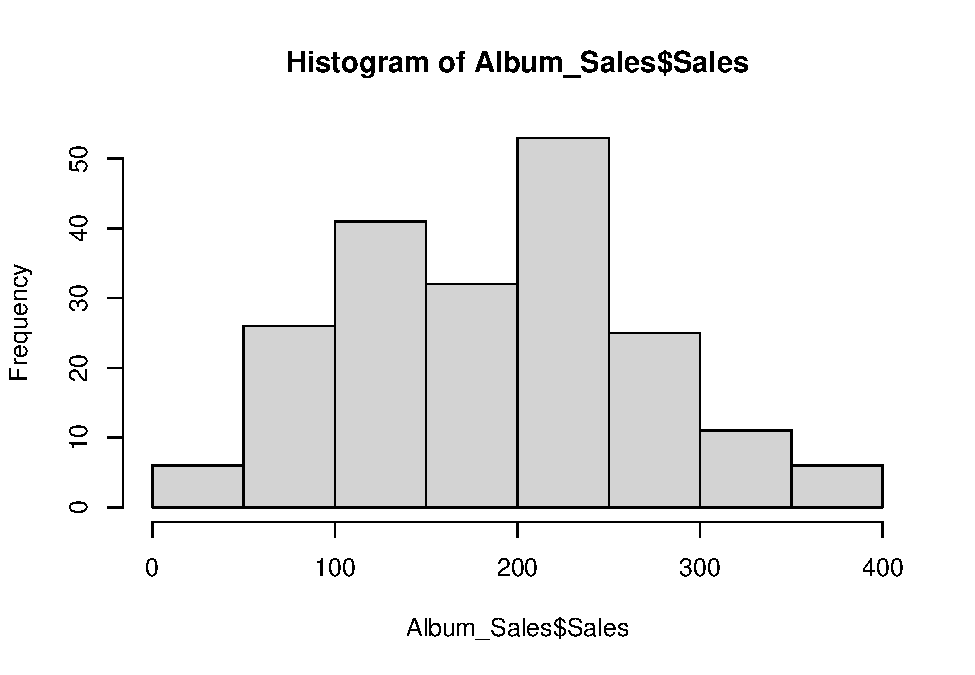
\includegraphics{PRBook_files/figure-latex/unnamed-chunk-34-1.pdf}

\hypertarget{assessing-skewness-of-distribution-2}{%
\subsection{Assessing skewness of distribution \#2}\label{assessing-skewness-of-distribution-2}}

\begin{itemize}
\tightlist
\item
  We can check raw skewness value using the \emph{skew()} command in the \textbf{psych} package
\end{itemize}

\begin{Shaded}
\begin{Highlighting}[]
\KeywordTok{library}\NormalTok{(psych)}
\end{Highlighting}
\end{Shaded}

\begin{verbatim}
## 
## Attaching package: 'psych'
\end{verbatim}

\begin{verbatim}
## The following object is masked from 'package:car':
## 
##     logit
\end{verbatim}

\begin{verbatim}
## The following objects are masked from 'package:ggplot2':
## 
##     %+%, alpha
\end{verbatim}

\begin{Shaded}
\begin{Highlighting}[]
\KeywordTok{skew}\NormalTok{(Album_Sales}\OperatorTok{$}\NormalTok{Sales)}
\end{Highlighting}
\end{Shaded}

\begin{verbatim}
## [1] 0.0432729
\end{verbatim}

\hypertarget{kurtosis}{%
\subsection{Kurtosis}\label{kurtosis}}

\begin{longtable}[]{@{}rrr@{}}
\toprule
informal term & technical name & kurtosis value\tabularnewline
\midrule
\endhead
``too flat'' & platykurtic & negative\tabularnewline
``just pointy enough'' & mesokurtic & zero\tabularnewline
``too pointy'' & leptokurtic & positive\tabularnewline
\bottomrule
\end{longtable}

\begin{Shaded}
\begin{Highlighting}[]
\KeywordTok{kurtosi}\NormalTok{(Album_Sales}\OperatorTok{$}\NormalTok{Sales)}
\end{Highlighting}
\end{Shaded}

\begin{verbatim}
## [1] -0.7157339
\end{verbatim}

\hypertarget{assessing-normality-of-distribution}{%
\subsection{Assessing normality of distribution}\label{assessing-normality-of-distribution}}

\begin{itemize}
\tightlist
\item
  We can use the shapiro-wilk test of normality
\item
  This is part of ``base'' r (no package needed)
\end{itemize}

\begin{Shaded}
\begin{Highlighting}[]
\KeywordTok{shapiro.test}\NormalTok{(Album_Sales}\OperatorTok{$}\NormalTok{Sales)}
\end{Highlighting}
\end{Shaded}

\begin{verbatim}
## 
##  Shapiro-Wilk normality test
## 
## data:  Album_Sales$Sales
## W = 0.98479, p-value = 0.02965
\end{verbatim}

\hypertarget{getting-and-overall-summary}{%
\section{Getting and overall summary}\label{getting-and-overall-summary}}

\hypertarget{summary---in-base-r}{%
\subsection{summary() - in ``base R''}\label{summary---in-base-r}}

\begin{Shaded}
\begin{Highlighting}[]
\KeywordTok{summary}\NormalTok{(Album_Sales)}
\end{Highlighting}
\end{Shaded}

\begin{verbatim}
##     Adverts             Sales          Airplay         Attract     
##  Min.   :   9.104   Min.   : 10.0   Min.   : 0.00   Min.   : 1.00  
##  1st Qu.: 215.918   1st Qu.:137.5   1st Qu.:19.75   1st Qu.: 6.00  
##  Median : 531.916   Median :200.0   Median :28.00   Median : 7.00  
##  Mean   : 614.412   Mean   :193.2   Mean   :27.50   Mean   : 6.77  
##  3rd Qu.: 911.226   3rd Qu.:250.0   3rd Qu.:36.00   3rd Qu.: 8.00  
##  Max.   :2271.860   Max.   :360.0   Max.   :63.00   Max.   :10.00  
##      Genre   
##  Country:46  
##  HipHop :53  
##  Metal  :48  
##  Pop    :53  
##              
## 
\end{verbatim}

\hypertarget{describe---in-the-psych-package-1}{%
\subsection{describe() - in the ``psych'' package \#1}\label{describe---in-the-psych-package-1}}

\begin{Shaded}
\begin{Highlighting}[]
\KeywordTok{describe}\NormalTok{(Album_Sales)}
\end{Highlighting}
\end{Shaded}

\begin{verbatim}
##         vars   n   mean     sd median trimmed    mad  min     max   range  skew
## Adverts    1 200 614.41 485.66 531.92  560.81 489.09  9.1 2271.86 2262.76  0.84
## Sales      2 200 193.20  80.70 200.00  192.69  88.96 10.0  360.00  350.00  0.04
## Airplay    3 200  27.50  12.27  28.00   27.46  11.86  0.0   63.00   63.00  0.06
## Attract    4 200   6.77   1.40   7.00    6.88   1.48  1.0   10.00    9.00 -1.27
## Genre*     5 200   2.54   1.12   3.00    2.55   1.48  1.0    4.00    3.00 -0.02
##         kurtosis    se
## Adverts     0.17 34.34
## Sales      -0.72  5.71
## Airplay    -0.09  0.87
## Attract     3.56  0.10
## Genre*     -1.37  0.08
\end{verbatim}

\hypertarget{describe---in-the-psych-package-2}{%
\subsection{describe() - in the ``psych'' package \#2}\label{describe---in-the-psych-package-2}}

\begin{itemize}
\tightlist
\item
  We can describe by factor variables
\end{itemize}

\begin{Shaded}
\begin{Highlighting}[]
\KeywordTok{describeBy}\NormalTok{(Album_Sales, }\DataTypeTok{group =}\NormalTok{ Album_Sales}\OperatorTok{$}\NormalTok{Genre)}
\end{Highlighting}
\end{Shaded}

\begin{verbatim}
## 
##  Descriptive statistics by group 
## group: Country
##         vars  n   mean     sd median trimmed    mad  min     max   range  skew
## Adverts    1 46 656.22 507.96 574.14  620.40 581.96  9.1 1985.12 1976.01  0.51
## Sales      2 46 201.74  73.64 210.00  200.79  66.72 60.0  360.00  300.00  0.03
## Airplay    3 46  29.07  10.53  28.00   28.50  11.12  9.0   54.00   45.00  0.44
## Attract    4 46   6.52   1.63   7.00    6.71   1.48  1.0   10.00    9.00 -1.49
## Genre*     5 46   1.00   0.00   1.00    1.00   0.00  1.0    1.00    0.00   NaN
##         kurtosis    se
## Adverts    -0.65 74.89
## Sales      -0.52 10.86
## Airplay    -0.10  1.55
## Attract     3.54  0.24
## Genre*       NaN  0.00
## ------------------------------------------------------------ 
## group: HipHop
##         vars  n   mean     sd median trimmed    mad   min  max   range  skew
## Adverts    1 53 606.32 452.84 601.43  568.33 501.36 10.65 2000 1989.35  0.70
## Sales      2 53 199.62  92.71 200.00  200.70 103.78 10.00  360  350.00 -0.10
## Airplay    3 53  28.09  13.86  30.00   28.33  14.83  0.00   55   55.00 -0.14
## Attract    4 53   6.96   1.13   7.00    7.00   1.48  3.00    9    6.00 -0.80
## Genre*     5 53   2.00   0.00   2.00    2.00   0.00  2.00    2    0.00   NaN
##         kurtosis    se
## Adverts     0.05 62.20
## Sales      -0.91 12.74
## Airplay    -0.83  1.90
## Attract     2.03  0.15
## Genre*       NaN  0.00
## ------------------------------------------------------------ 
## group: Metal
##         vars  n   mean     sd median trimmed    mad  min     max   range  skew
## Adverts    1 48 693.45 534.06  593.0  640.19 521.34 45.3 2271.86 2226.56  0.92
## Sales      2 48 197.71  75.18  200.0  198.25  88.96 40.0  340.00  300.00 -0.07
## Airplay    3 48  27.96  11.37   27.5   28.00  11.12  2.0   57.00   55.00  0.02
## Attract    4 48   6.85   1.34    7.0    6.90   1.48  2.0    9.00    7.00 -0.84
## Genre*     5 48   3.00   0.00    3.0    3.00   0.00  3.0    3.00    0.00   NaN
##         kurtosis    se
## Adverts     0.21 77.08
## Sales      -0.94 10.85
## Airplay    -0.26  1.64
## Attract     1.74  0.19
## Genre*       NaN  0.00
## ------------------------------------------------------------ 
## group: Pop
##         vars  n   mean     sd median trimmed    mad   min     max   range  skew
## Adverts    1 53 514.63 446.04  429.5  453.85 438.01 15.31 1789.66 1774.35  1.01
## Sales      2 53 175.28  77.92  160.0  171.86  88.96 40.00  360.00  320.00  0.34
## Airplay    3 53  25.13  12.75   26.0   25.02  11.86  1.00   63.00   62.00  0.25
## Attract    4 53   6.72   1.47    7.0    6.81   1.48  1.00    9.00    8.00 -1.11
## Genre*     5 53   4.00   0.00    4.0    4.00   0.00  4.00    4.00    0.00   NaN
##         kurtosis    se
## Adverts     0.27 61.27
## Sales      -0.67 10.70
## Airplay     0.46  1.75
## Attract     2.51  0.20
## Genre*       NaN  0.00
\end{verbatim}

\hypertarget{basic-statistical-tests-more-detail-in-later-sections}{%
\section{Basic statistical tests (more detail in later sections)}\label{basic-statistical-tests-more-detail-in-later-sections}}

\hypertarget{corrleation}{%
\subsection{Corrleation}\label{corrleation}}

``Is there a relationship between advert spend and sales?''

\begin{itemize}
\tightlist
\item
  We would use an correlational analysis to answer this question
\end{itemize}

\begin{Shaded}
\begin{Highlighting}[]
\KeywordTok{plot}\NormalTok{(Album_Sales}\OperatorTok{$}\NormalTok{Sales,Album_Sales}\OperatorTok{$}\NormalTok{Adverts)}
\end{Highlighting}
\end{Shaded}

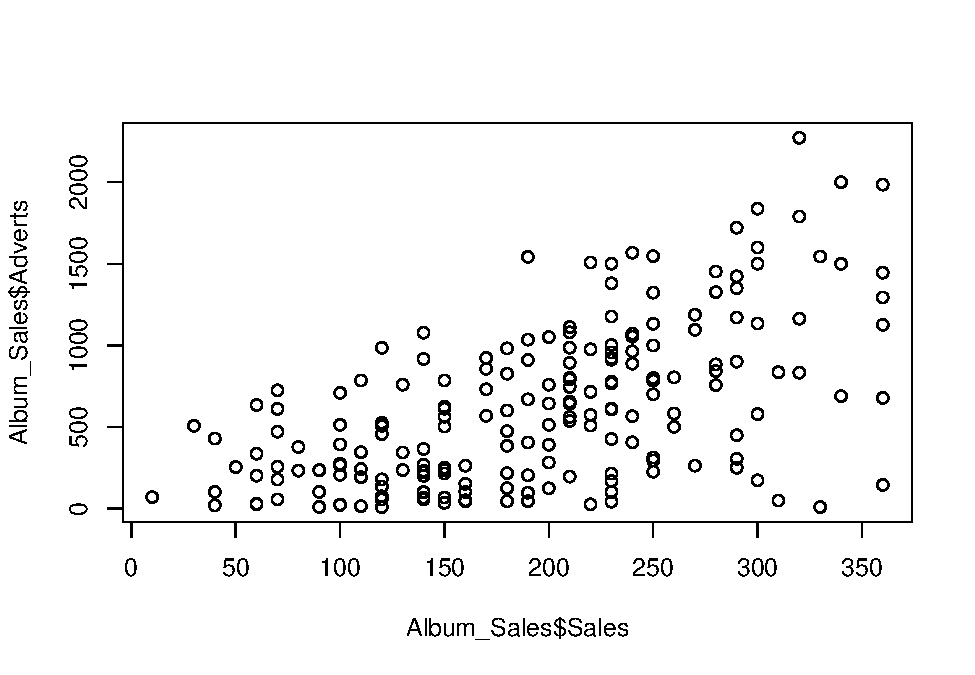
\includegraphics{PRBook_files/figure-latex/unnamed-chunk-41-1.pdf}

``Is there a relationship between advert spend and sales?''

\begin{itemize}
\tightlist
\item
  We would use an correlational analysis to answer this question
\end{itemize}

\begin{Shaded}
\begin{Highlighting}[]
\KeywordTok{cor.test}\NormalTok{(Album_Sales}\OperatorTok{$}\NormalTok{Sales,Album_Sales}\OperatorTok{$}\NormalTok{Adverts)}
\end{Highlighting}
\end{Shaded}

\begin{verbatim}
## 
##  Pearson's product-moment correlation
## 
## data:  Album_Sales$Sales and Album_Sales$Adverts
## t = 9.9793, df = 198, p-value < 2.2e-16
## alternative hypothesis: true correlation is not equal to 0
## 95 percent confidence interval:
##  0.4781207 0.6639409
## sample estimates:
##       cor 
## 0.5784877
\end{verbatim}

\hypertarget{tests-of-difference---t-test}{%
\subsection{Tests of difference - t-test}\label{tests-of-difference---t-test}}

``Is there a significant difference in sales between the Country and Hip-hop musical genres?''

\begin{itemize}
\tightlist
\item
  We would use a t-test to answer this question
\end{itemize}

\begin{Shaded}
\begin{Highlighting}[]
\NormalTok{myTtestData <-}\StringTok{ }\NormalTok{Album_Sales }\OperatorTok\StringTok{ }\KeywordTok{filter}\NormalTok{(Genre }\OperatorTok{==}\StringTok{ }\KeywordTok{c}\NormalTok{(}\StringTok{"Country"}\NormalTok{, }\StringTok{"HipHop"}\NormalTok{))}

\KeywordTok{t.test}\NormalTok{(myTtestData}\OperatorTok{$}\NormalTok{Sales }\OperatorTok{~}\StringTok{ }\NormalTok{myTtestData}\OperatorTok{$}\NormalTok{Genre)}
\end{Highlighting}
\end{Shaded}

\begin{verbatim}
## 
##  Welch Two Sample t-test
## 
## data:  myTtestData$Sales by myTtestData$Genre
## t = 0.80489, df = 40.62, p-value = 0.4256
## alternative hypothesis: true difference in means is not equal to 0
## 95 percent confidence interval:
##  -27.80146  64.62904
## sample estimates:
## mean in group Country  mean in group HipHop 
##              216.0000              197.5862
\end{verbatim}

\hypertarget{tests-of-difference---anova}{%
\subsection{Tests of difference - ANOVA}\label{tests-of-difference---anova}}

``Is there a significant difference in sales between all musical genres?''

\begin{itemize}
\tightlist
\item
  We would use an ANOVA to answer this question
\end{itemize}

\begin{Shaded}
\begin{Highlighting}[]
\NormalTok{myAnova <-}\StringTok{ }\KeywordTok{aov}\NormalTok{(Album_Sales}\OperatorTok{$}\NormalTok{Sales }\OperatorTok{~}\StringTok{ }\NormalTok{Album_Sales}\OperatorTok{$}\NormalTok{Genre)}
\KeywordTok{summary}\NormalTok{(myAnova)}
\end{Highlighting}
\end{Shaded}

\begin{verbatim}
##                    Df  Sum Sq Mean Sq F value Pr(>F)
## Album_Sales$Genre   3   23530    7843   1.208  0.308
## Residuals         196 1272422    6492
\end{verbatim}

\hypertarget{graphing-and-data-visualisation-with-r}{%
\chapter{Graphing and data visualisation with R}\label{graphing-and-data-visualisation-with-r}}

\hypertarget{presenting-data-visually}{%
\section{Presenting data visually}\label{presenting-data-visually}}

\hypertarget{by-the-end-of-this-section-you-will-be-able-to-1}{%
\section{By the end of this section, you will be able to:}\label{by-the-end-of-this-section-you-will-be-able-to-1}}

\begin{itemize}
\tightlist
\item
  Describe the ggplot ``grammar of visualisation'': coordinates and geoms
\item
  Write a graph function to display multiple variables on a plot
\item
  Amend the titles and legends of a plot
\item
  Save plots in PDF or image formats
\end{itemize}

\hypertarget{the-grammar-of-visualisation}{%
\section{The ``grammar of visualisation''}\label{the-grammar-of-visualisation}}

\begin{itemize}
\tightlist
\item
  Graphs are made up of 3 components:

  \begin{itemize}
  \tightlist
  \item
    A dataset
  \item
    A coordinate system
  \item
    Visual marks to represent data \textbf{(geoms)}
  \end{itemize}
\end{itemize}

The ``grammar of visualisation'' \#2

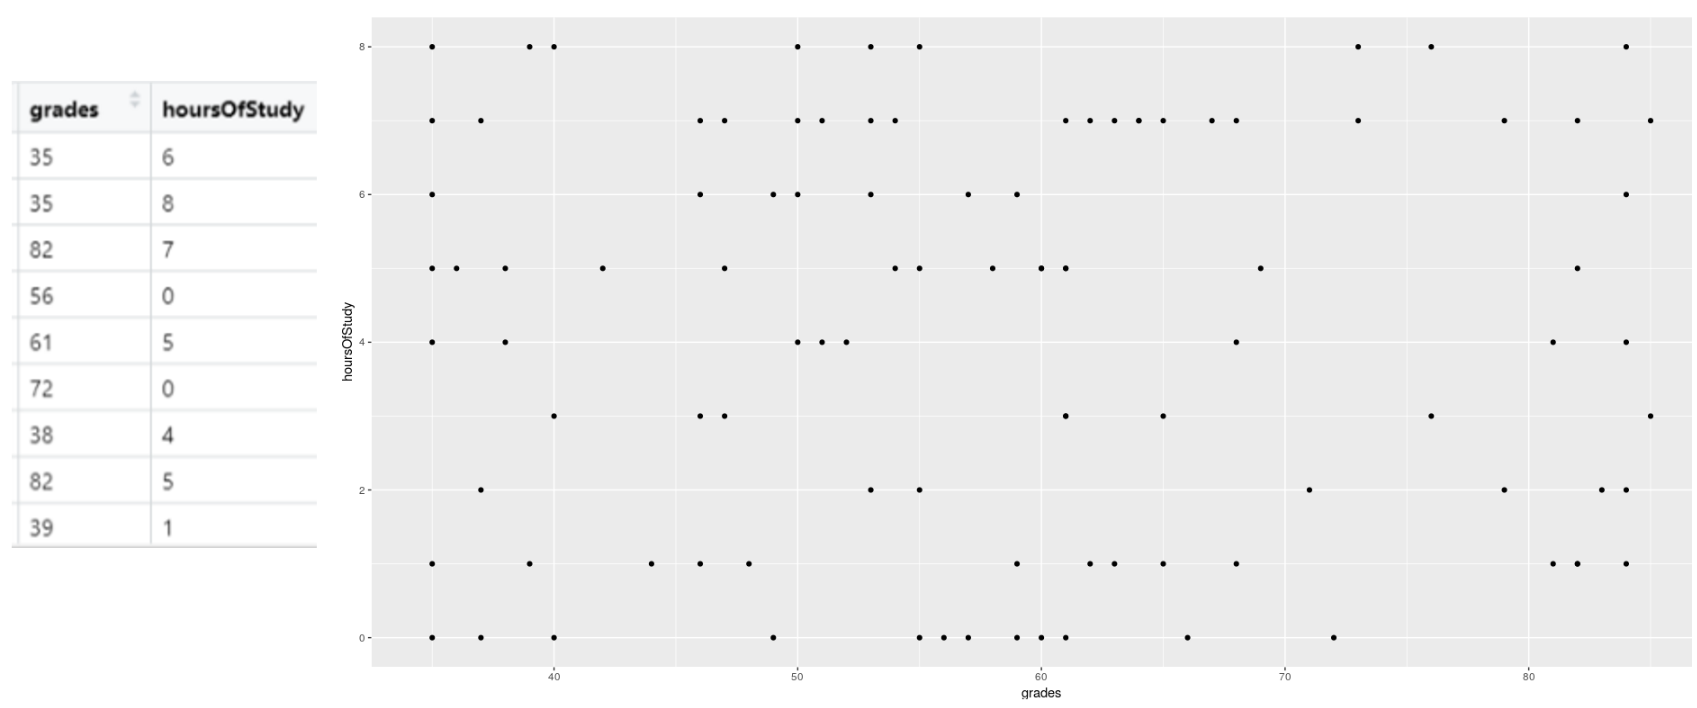
\includegraphics[width=1\linewidth]{img/ggplot1}

\begin{itemize}
\tightlist
\item
  In the above example, the dataset is the \emph{studentData} that we used previously.
\item
  The \emph{grades} variable is mapped to the X axis
\item
  The \emph{hoursOfStudy} variable is mapped to the Y axis
\end{itemize}

\hypertarget{how-to-code-a-graph}{%
\section{How to code a graph}\label{how-to-code-a-graph}}

\begin{itemize}
\tightlist
\item
  The graph is created using the following code:
\end{itemize}

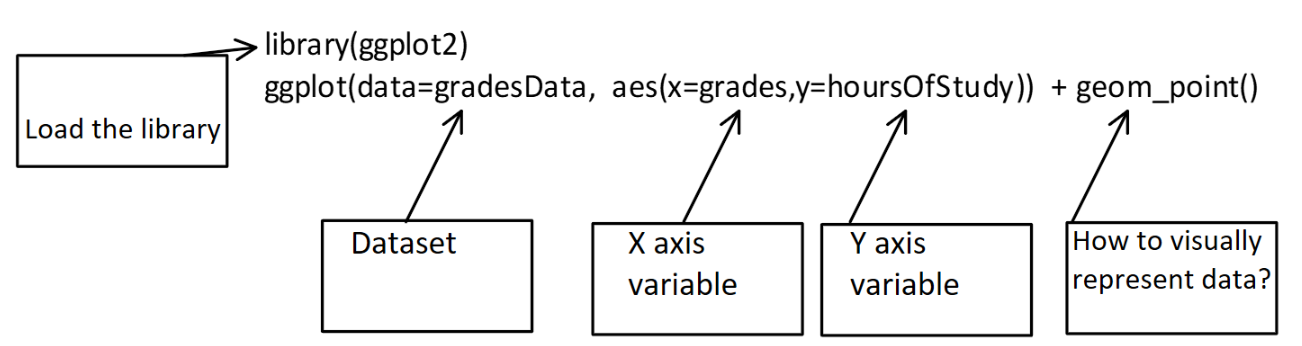
\includegraphics[width=1\linewidth]{img/ggplot2}

\begin{itemize}
\tightlist
\item
  In this code, we specify the dataset, the variables for the X and Y axes and the \textbf{geom} that will represent the data points visually (in this case, each datum is a point)
\end{itemize}

\hypertarget{the-graph-output}{%
\section{The graph output}\label{the-graph-output}}

\begin{Shaded}
\begin{Highlighting}[]
\KeywordTok{library}\NormalTok{(ggplot2)}

\KeywordTok{ggplot}\NormalTok{(}\DataTypeTok{data=}\NormalTok{studentData, }\KeywordTok{aes}\NormalTok{(}\DataTypeTok{x=}\NormalTok{grades,}\DataTypeTok{y=}\NormalTok{hoursOfStudy)) }\OperatorTok{+}\StringTok{ }\KeywordTok{geom_point}\NormalTok{()}
\end{Highlighting}
\end{Shaded}

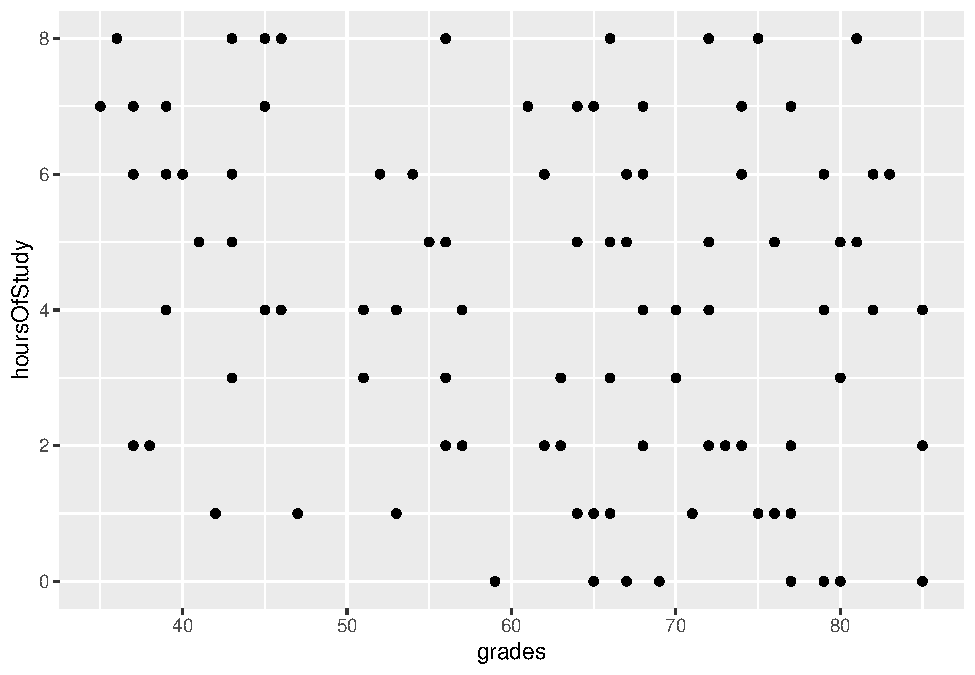
\includegraphics{PRBook_files/figure-latex/unnamed-chunk-47-1.pdf}

\hypertarget{changing-the-geoms-leads-to-different-visualisations}{%
\section{Changing the geoms leads to different visualisations}\label{changing-the-geoms-leads-to-different-visualisations}}

\begin{itemize}
\tightlist
\item
  If we change from points to lines, for example we get a different plot:
\end{itemize}

\begin{Shaded}
\begin{Highlighting}[]
\KeywordTok{library}\NormalTok{(ggplot2)}

\KeywordTok{ggplot}\NormalTok{(}\DataTypeTok{data=}\NormalTok{studentData, }\KeywordTok{aes}\NormalTok{(}\DataTypeTok{x=}\NormalTok{grades,}\DataTypeTok{y=}\NormalTok{hoursOfStudy)) }\OperatorTok{+}\StringTok{ }\KeywordTok{geom_line}\NormalTok{()}
\end{Highlighting}
\end{Shaded}

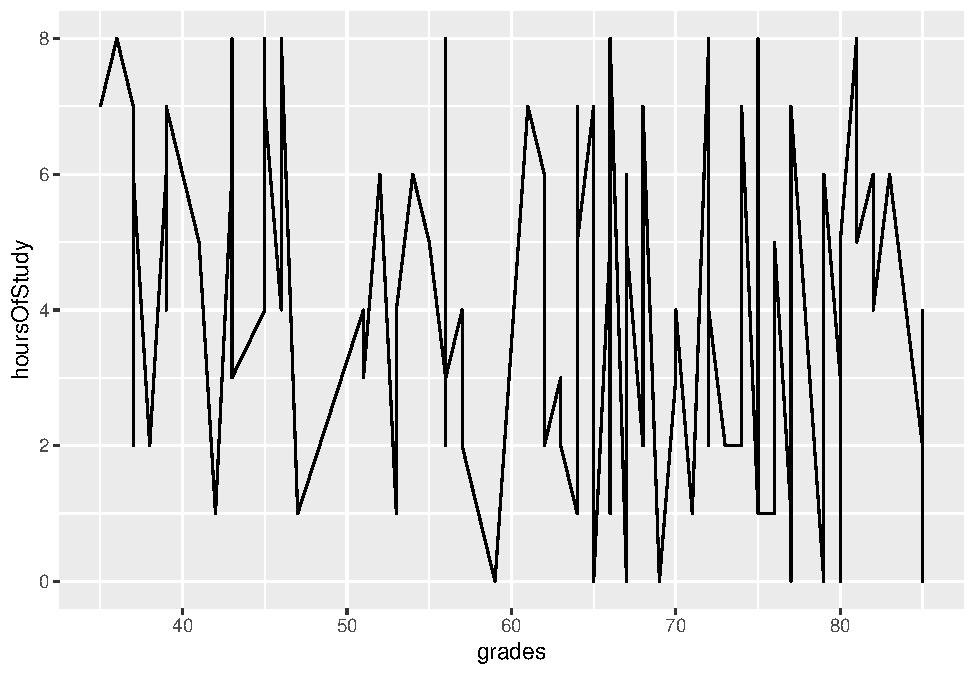
\includegraphics{PRBook_files/figure-latex/unnamed-chunk-48-1.pdf}

\hypertarget{it-is-possible-to-represent-more-variables-on-the-plot}{%
\section{It is possible to represent more variables on the plot}\label{it-is-possible-to-represent-more-variables-on-the-plot}}

\begin{itemize}
\tightlist
\item
  By specifying that colours of our points should be attached to the \textbf{route} variable, the data is now colour-coded
\end{itemize}

\begin{Shaded}
\begin{Highlighting}[]
\KeywordTok{library}\NormalTok{(ggplot2)}

\KeywordTok{ggplot}\NormalTok{(}\DataTypeTok{data=}\NormalTok{studentData, }\KeywordTok{aes}\NormalTok{(}\DataTypeTok{x=}\NormalTok{grades,}\DataTypeTok{y=}\NormalTok{hoursOfStudy)) }\OperatorTok{+}\StringTok{ }\KeywordTok{geom_point}\NormalTok{(}\KeywordTok{aes}\NormalTok{(}\DataTypeTok{color =}\NormalTok{ route))}
\end{Highlighting}
\end{Shaded}

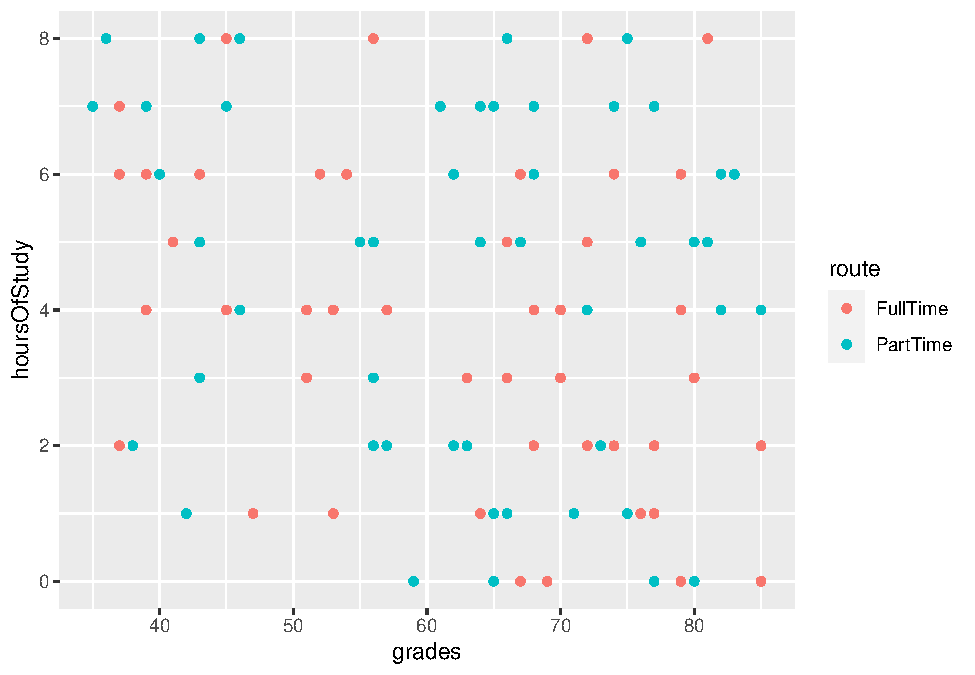
\includegraphics{PRBook_files/figure-latex/unnamed-chunk-49-1.pdf}

\hypertarget{it-is-possible-to-represent-more-variables-on-the-plot-2}{%
\section{It is possible to represent more variables on the plot \#2}\label{it-is-possible-to-represent-more-variables-on-the-plot-2}}

\begin{itemize}
\tightlist
\item
  By specifying that size of our points should be attached to the \textbf{satisfactionLevel} variable, the size of the points adjusts
\end{itemize}

\begin{Shaded}
\begin{Highlighting}[]
\KeywordTok{library}\NormalTok{(ggplot2)}

\KeywordTok{ggplot}\NormalTok{(}\DataTypeTok{data=}\NormalTok{studentData, }\KeywordTok{aes}\NormalTok{(}\DataTypeTok{x=}\NormalTok{grades,}\DataTypeTok{y=}\NormalTok{hoursOfStudy)) }\OperatorTok{+}\StringTok{ }\KeywordTok{geom_point}\NormalTok{(}\KeywordTok{aes}\NormalTok{(}\DataTypeTok{color =}\NormalTok{ route, }\DataTypeTok{size=}\NormalTok{satisfactionLevel))}
\end{Highlighting}
\end{Shaded}

\begin{verbatim}
## Warning: Using size for a discrete variable is not advised.
\end{verbatim}

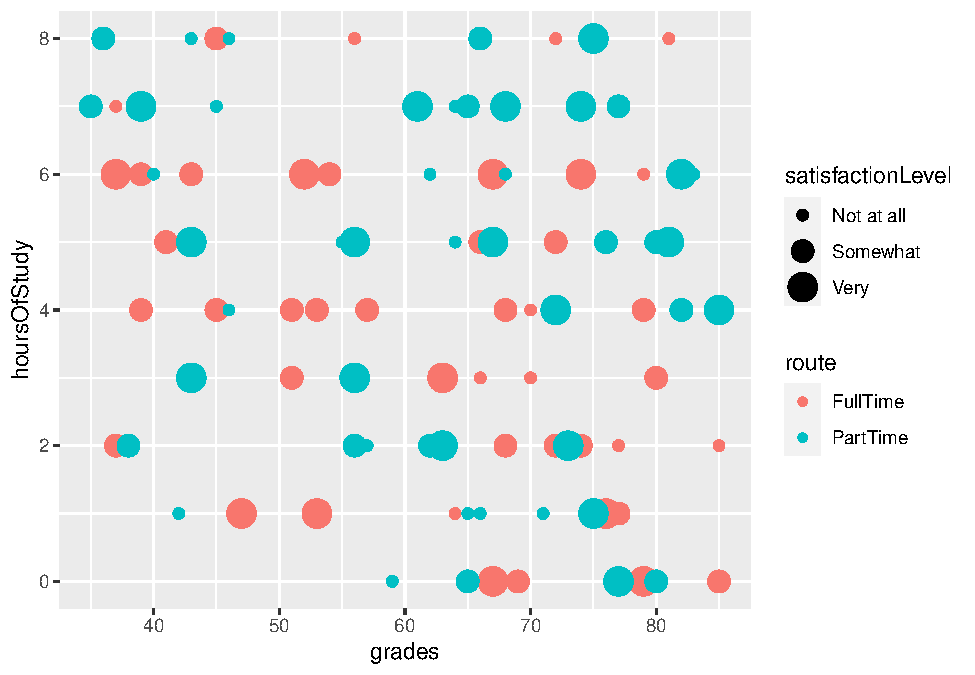
\includegraphics{PRBook_files/figure-latex/unnamed-chunk-50-1.pdf}

\hypertarget{it-is-possible-to-represent-more-variables-on-the-plot-3}{%
\section{It is possible to represent more variables on the plot \#3}\label{it-is-possible-to-represent-more-variables-on-the-plot-3}}

\begin{itemize}
\tightlist
\item
  By specifying that shape of our points should be attached to the \textbf{hasDependents} variable, the shape of the points changes accordingly
\end{itemize}

\begin{Shaded}
\begin{Highlighting}[]
\KeywordTok{library}\NormalTok{(ggplot2)}

\KeywordTok{ggplot}\NormalTok{(}\DataTypeTok{data=}\NormalTok{studentData, }\KeywordTok{aes}\NormalTok{(}\DataTypeTok{x=}\NormalTok{grades,}\DataTypeTok{y=}\NormalTok{hoursOfStudy)) }\OperatorTok{+}\StringTok{ }\KeywordTok{geom_point}\NormalTok{(}\KeywordTok{aes}\NormalTok{(}\DataTypeTok{color =}\NormalTok{ route, }\DataTypeTok{size=}\NormalTok{satisfactionLevel, }\DataTypeTok{shape=}\NormalTok{hasDepdendants))}
\end{Highlighting}
\end{Shaded}

\begin{verbatim}
## Warning: Using size for a discrete variable is not advised.
\end{verbatim}

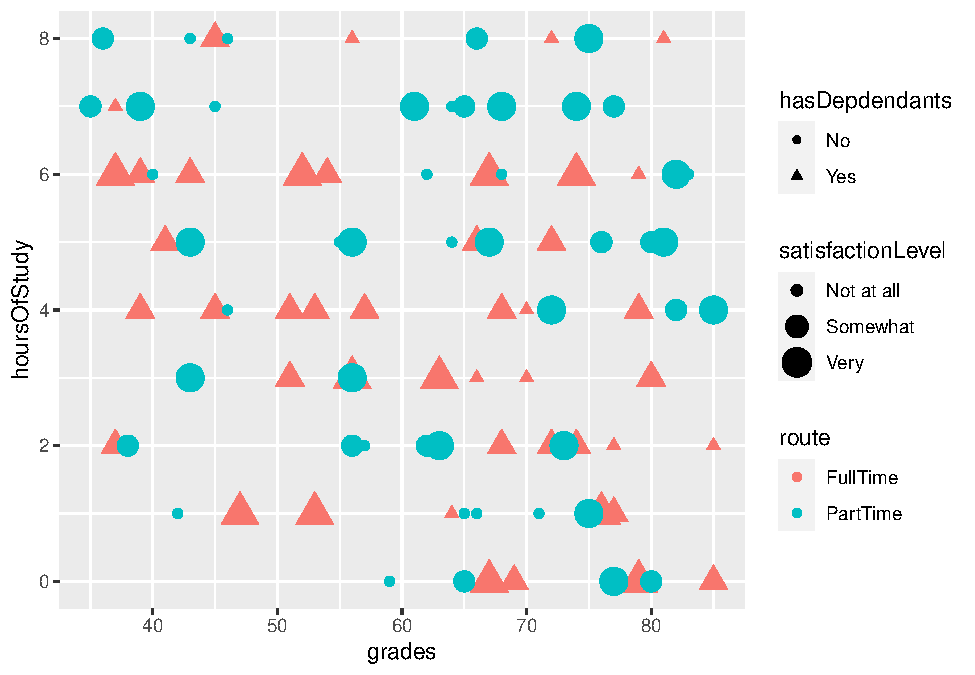
\includegraphics{PRBook_files/figure-latex/unnamed-chunk-51-1.pdf}

\hypertarget{plotting-summaries-of-data}{%
\section{Plotting summaries of data}\label{plotting-summaries-of-data}}

\begin{itemize}
\tightlist
\item
  We can summarise the data (e.g.~get the mean or sd) using the \emph{stat\_summary()} function
\item
  Below we are making a bar chart with the mean grade for each route
\end{itemize}

\begin{Shaded}
\begin{Highlighting}[]
\KeywordTok{ggplot}\NormalTok{(}\DataTypeTok{data=}\NormalTok{studentData, }\KeywordTok{aes}\NormalTok{(}\DataTypeTok{x=}\NormalTok{route, }\DataTypeTok{y=}\NormalTok{ grades, }\DataTypeTok{fill=}\NormalTok{route)) }\OperatorTok{+}\StringTok{ }\KeywordTok{stat_summary}\NormalTok{(}\DataTypeTok{fun.y =} \StringTok{"mean"}\NormalTok{, }\DataTypeTok{geom =} \StringTok{"bar"}\NormalTok{)}
\end{Highlighting}
\end{Shaded}

\begin{verbatim}
## Warning: `fun.y` is deprecated. Use `fun` instead.
\end{verbatim}

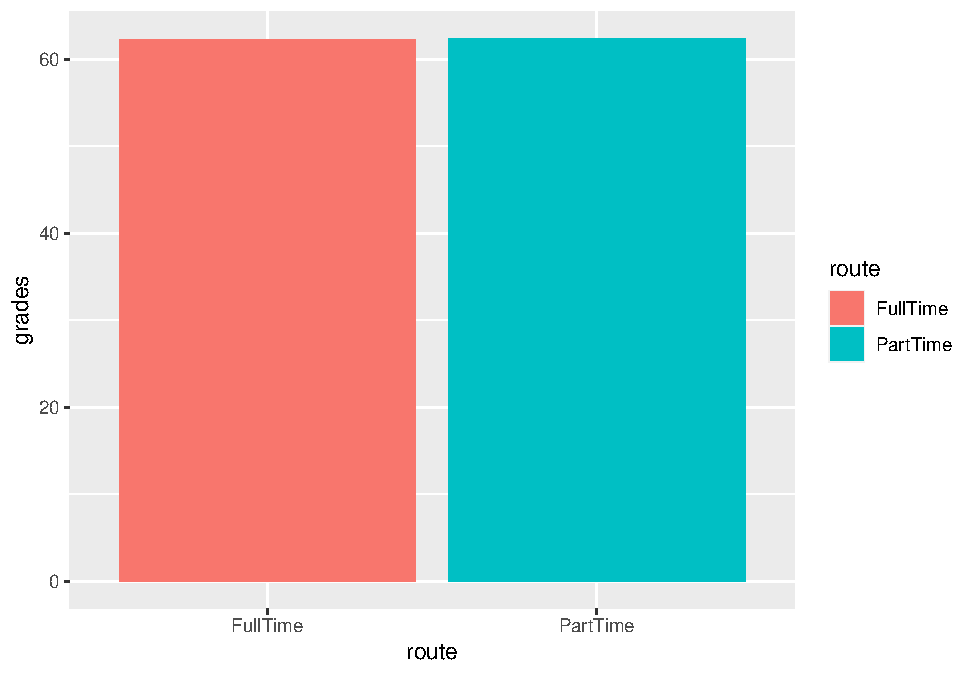
\includegraphics{PRBook_files/figure-latex/unnamed-chunk-52-1.pdf}

\hypertarget{changing-the-axis-labels-and-title-on-a-plot}{%
\section{Changing the axis labels and title on a plot}\label{changing-the-axis-labels-and-title-on-a-plot}}

We can change the axis labels and title using the \textbf{labs()} command:

\begin{verbatim}
labs(x="Student Grade", y="Hours of Study", title = "Scattterplot of student data")
\end{verbatim}

\begin{Shaded}
\begin{Highlighting}[]
\KeywordTok{library}\NormalTok{(ggplot2)}

\KeywordTok{ggplot}\NormalTok{(}\DataTypeTok{data=}\NormalTok{studentData, }\KeywordTok{aes}\NormalTok{(}\DataTypeTok{x=}\NormalTok{grades,}\DataTypeTok{y=}\NormalTok{hoursOfStudy)) }\OperatorTok{+}\StringTok{ }\KeywordTok{geom_point}\NormalTok{(}\KeywordTok{aes}\NormalTok{(}\DataTypeTok{color =}\NormalTok{ route, }\DataTypeTok{size=}\NormalTok{satisfactionLevel, }\DataTypeTok{shape=}\NormalTok{hasDepdendants)) }\OperatorTok{+}\StringTok{ }\KeywordTok{labs}\NormalTok{(}\DataTypeTok{x=}\StringTok{"Student Grade"}\NormalTok{, }\DataTypeTok{y=}\StringTok{"Hours of Study"}\NormalTok{, }\DataTypeTok{title =} \StringTok{"Scattterplot of studentdata"}\NormalTok{)}
\end{Highlighting}
\end{Shaded}

\begin{verbatim}
## Warning: Using size for a discrete variable is not advised.
\end{verbatim}

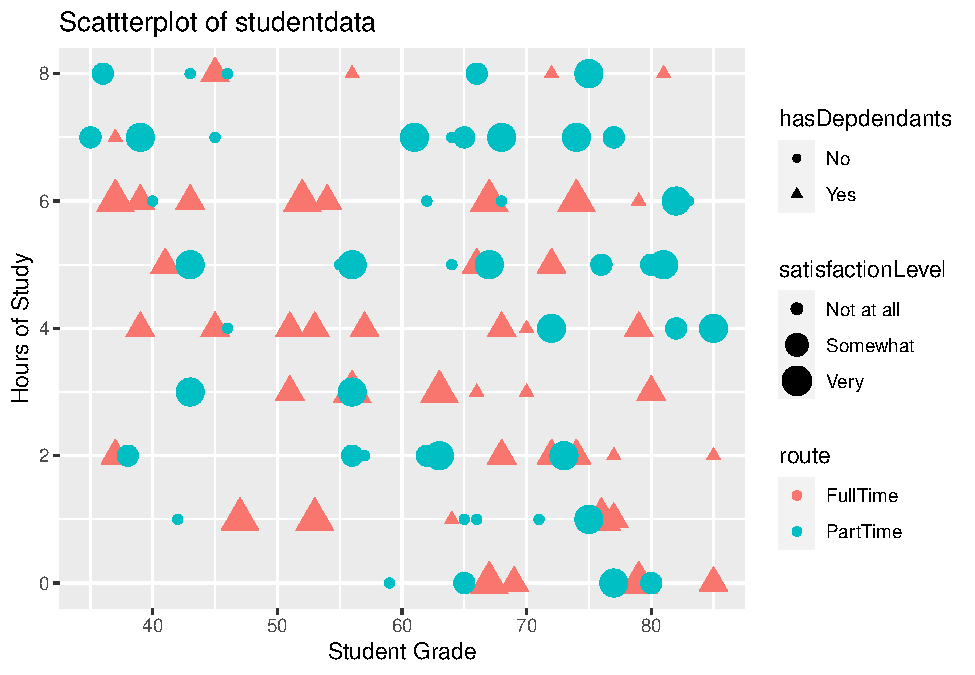
\includegraphics{PRBook_files/figure-latex/unnamed-chunk-53-1.pdf}

\hypertarget{changing-the-legend-on-a-plot}{%
\section{Changing the legend on a plot}\label{changing-the-legend-on-a-plot}}

To change the legend, we use the \textbf{labs()} command too, and reference the relevant property (e.g.~size, shape, colour)

\begin{verbatim}
labs(x="Student Grade", y="Hours of Study", title = "Scattterplot of student data", color="Route of study", size="Satisfaction level", shape="Has dependents?")
\end{verbatim}

\begin{Shaded}
\begin{Highlighting}[]
\KeywordTok{library}\NormalTok{(ggplot2)}

  \KeywordTok{ggplot}\NormalTok{(}\DataTypeTok{data=}\NormalTok{studentData, }\KeywordTok{aes}\NormalTok{(}\DataTypeTok{x=}\NormalTok{grades,}\DataTypeTok{y=}\NormalTok{hoursOfStudy)) }\OperatorTok{+}\StringTok{ }
\StringTok{    }\KeywordTok{geom_point}\NormalTok{(}\KeywordTok{aes}\NormalTok{(}\DataTypeTok{color =}\NormalTok{ route, }\DataTypeTok{size=}\NormalTok{satisfactionLevel, }\DataTypeTok{shape=}\NormalTok{hasDepdendants)) }\OperatorTok{+}
\StringTok{  }\KeywordTok{labs}\NormalTok{(}\DataTypeTok{x=}\StringTok{"Student Grade"}\NormalTok{, }\DataTypeTok{y=}\StringTok{"Hours of Study"}\NormalTok{, }\DataTypeTok{title =} \StringTok{"Scattterplot of studentdata"}\NormalTok{, }\DataTypeTok{color=}\StringTok{"Route of study"}\NormalTok{, }\DataTypeTok{size=}\StringTok{"Satisfaction level"}\NormalTok{, }\DataTypeTok{shape=}\StringTok{"Has dependents?"}\NormalTok{)}
\end{Highlighting}
\end{Shaded}

\begin{verbatim}
## Warning: Using size for a discrete variable is not advised.
\end{verbatim}

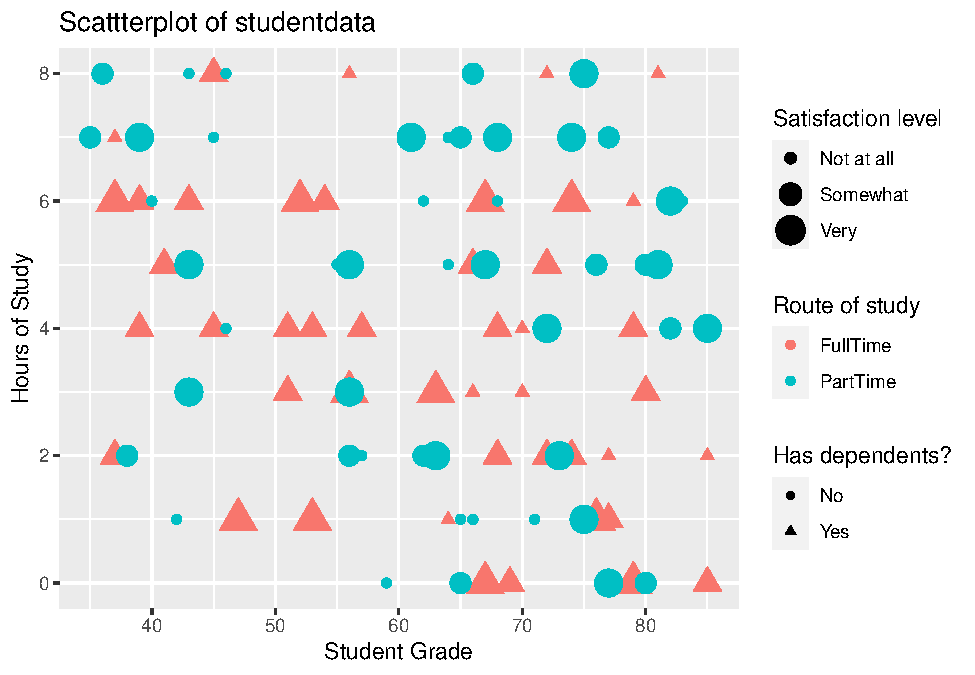
\includegraphics{PRBook_files/figure-latex/unnamed-chunk-54-1.pdf}

\hypertarget{storing-plots-to-be-recalled-later}{%
\section{Storing plots to be recalled later}\label{storing-plots-to-be-recalled-later}}

\begin{itemize}
\tightlist
\item
  Plots can be assigned to objects in R and recalled later, just like any other piece of data
\end{itemize}

\begin{Shaded}
\begin{Highlighting}[]
\KeywordTok{library}\NormalTok{(ggplot2)}

\CommentTok{## Create plot and store it as "myPlot" object}

\NormalTok{myPlot <-}\StringTok{ }\KeywordTok{ggplot}\NormalTok{(}\DataTypeTok{data=}\NormalTok{studentData, }\KeywordTok{aes}\NormalTok{(}\DataTypeTok{x=}\NormalTok{grades,}\DataTypeTok{y=}\NormalTok{hoursOfStudy)) }\OperatorTok{+}
\StringTok{  }\KeywordTok{geom_point}\NormalTok{(}\KeywordTok{aes}\NormalTok{(}\DataTypeTok{color =}\NormalTok{ route, }\DataTypeTok{size=}\NormalTok{satisfactionLevel, }\DataTypeTok{shape=}\NormalTok{hasDepdendants)) }\OperatorTok{+}
\StringTok{  }\KeywordTok{labs}\NormalTok{(}\DataTypeTok{x=}\StringTok{"Student Grade"}\NormalTok{, }\DataTypeTok{y=}\StringTok{"Hours of Study"}\NormalTok{, }\DataTypeTok{title =} \StringTok{"Scattterplot of studentdata"}\NormalTok{, }\DataTypeTok{color=}\StringTok{"Route of study"}\NormalTok{, }\DataTypeTok{size=}\StringTok{"Satisfaction level"}\NormalTok{, }\DataTypeTok{shape=}\StringTok{"Has dependents?"}\NormalTok{)}
\end{Highlighting}
\end{Shaded}

\hypertarget{recalling-a-stored-plot}{%
\section{Recalling a stored plot}\label{recalling-a-stored-plot}}

\begin{Shaded}
\begin{Highlighting}[]
 \CommentTok{#Recall myPlot}
\NormalTok{myPlot}
\end{Highlighting}
\end{Shaded}

\begin{verbatim}
## Warning: Using size for a discrete variable is not advised.
\end{verbatim}

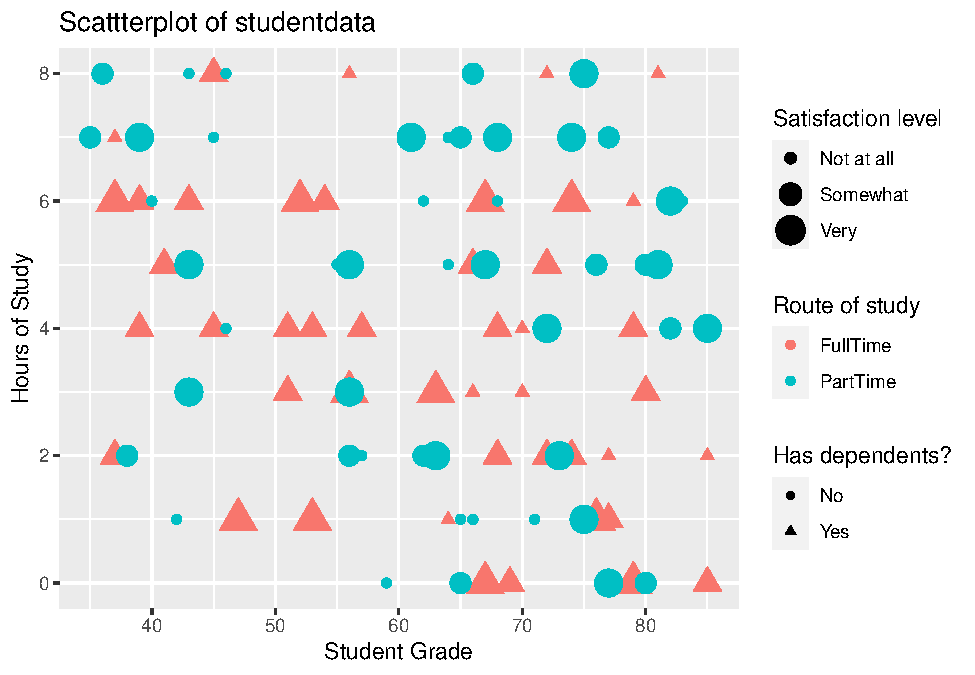
\includegraphics{PRBook_files/figure-latex/unnamed-chunk-56-1.pdf}

\hypertarget{saving-plots-1}{%
\section{Saving plots \# 1}\label{saving-plots-1}}

\begin{itemize}
\tightlist
\item
  Plots can be save using the \textbf{export} button in the plots tab
\end{itemize}

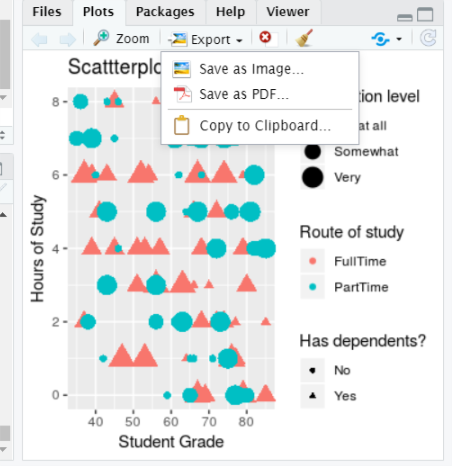
\includegraphics[width=1\linewidth]{img/savePlot1}

\hypertarget{plots-can-also-be-saved-using-code}{%
\section{Plots can also be saved using code}\label{plots-can-also-be-saved-using-code}}

\begin{itemize}
\tightlist
\item
  You might want to include code to save your plot in a script, for example
\item
  This can allow greater control over the output file and plot dimensions:
\end{itemize}

\begin{Shaded}
\begin{Highlighting}[]
\KeywordTok{ggsave}\NormalTok{(}\DataTypeTok{plot=}\NormalTok{ myPlot, }\DataTypeTok{file=}\StringTok{"myPlot.pdf"}\NormalTok{, }\DataTypeTok{width =} \DecValTok{4}\NormalTok{, }\DataTypeTok{height =} \DecValTok{4}\NormalTok{)}
\end{Highlighting}
\end{Shaded}

\begin{verbatim}
## Warning: Using size for a discrete variable is not advised.
\end{verbatim}

\begin{Shaded}
\begin{Highlighting}[]
\KeywordTok{ggsave}\NormalTok{(}\DataTypeTok{plot=}\NormalTok{ myPlot, }\DataTypeTok{file=}\StringTok{"myPlot.png"}\NormalTok{, }\DataTypeTok{width =} \DecValTok{4}\NormalTok{, }\DataTypeTok{height =} \DecValTok{4}\NormalTok{, }\DataTypeTok{units=}\StringTok{"cm"}\NormalTok{, }\DataTypeTok{dpi=}\DecValTok{320}\NormalTok{)}
\end{Highlighting}
\end{Shaded}

\begin{verbatim}
## Warning: Using size for a discrete variable is not advised.
\end{verbatim}

\hypertarget{correlation}{%
\chapter{Correlation}\label{correlation}}

\hypertarget{what-is-correlation}{%
\section{What is Correlation?}\label{what-is-correlation}}

\begin{itemize}
\tightlist
\item
  The relationship between 2 variables
\item
  Question: Is treatment duration related to aggression levels?
\end{itemize}

\hypertarget{how-is-correlation-calculated}{%
\section{How is correlation calculated?}\label{how-is-correlation-calculated}}

\begin{itemize}
\tightlist
\item
  Think of this as covariance divided by individual variance
\item
  If the changes are consistent with both variables, the final value will be higher
\end{itemize}

\begin{center}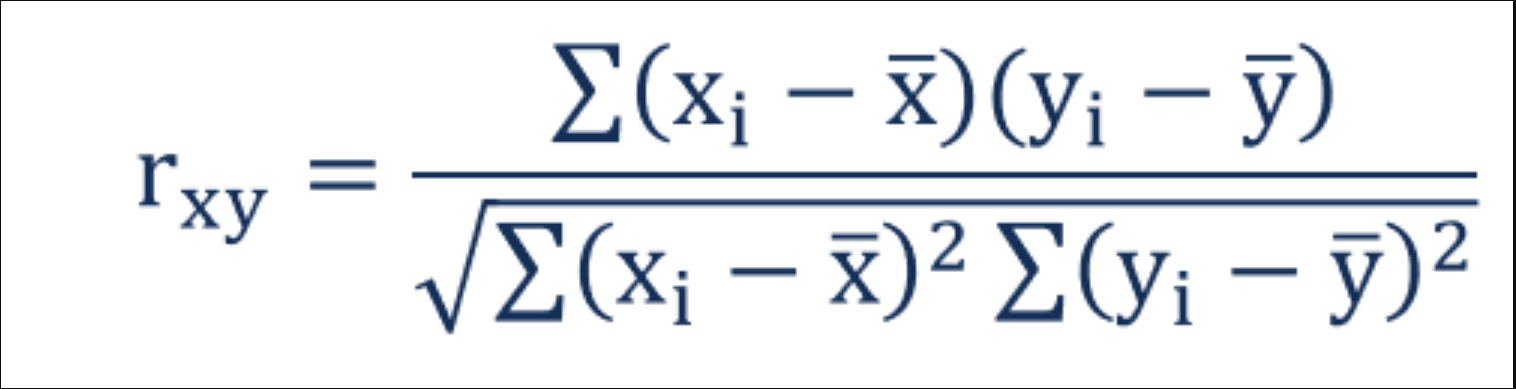
\includegraphics[width=1\linewidth]{img/correlation} \end{center}

\begin{center}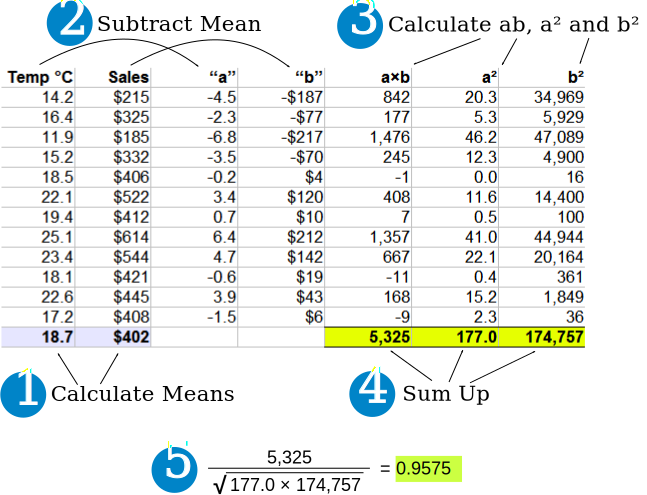
\includegraphics[width=11.32in,height=1\textheight]{img/corcalc} \end{center}

\hypertarget{running-correlation-in-r}{%
\section{Running correlation in R}\label{running-correlation-in-r}}

\begin{itemize}
\tightlist
\item
  Step 1: Check assumptions

  \begin{itemize}
  \tightlist
  \item
    Data,distribution,linearity
  \end{itemize}
\item
  Step 2: Run correlation
\item
  Step 3: Check R value
\item
  Step 4: Check significance
\end{itemize}

\hypertarget{check-assumptions-data}{%
\subsection{Check assumptions: data}\label{check-assumptions-data}}

\begin{itemize}
\tightlist
\item
  Parametric tests require interval or ratio data
\item
  If the data are ordinal then a non-parametric correlation is used
\end{itemize}

\begin{quote}
What type of data are treatment duration and aggression level?
\end{quote}

\hypertarget{check-assumptions-distribution}{%
\subsection{Check assumptions: distribution}\label{check-assumptions-distribution}}

\begin{itemize}
\tightlist
\item
  Parametric tests require normally distributed data
\end{itemize}

\begin{center}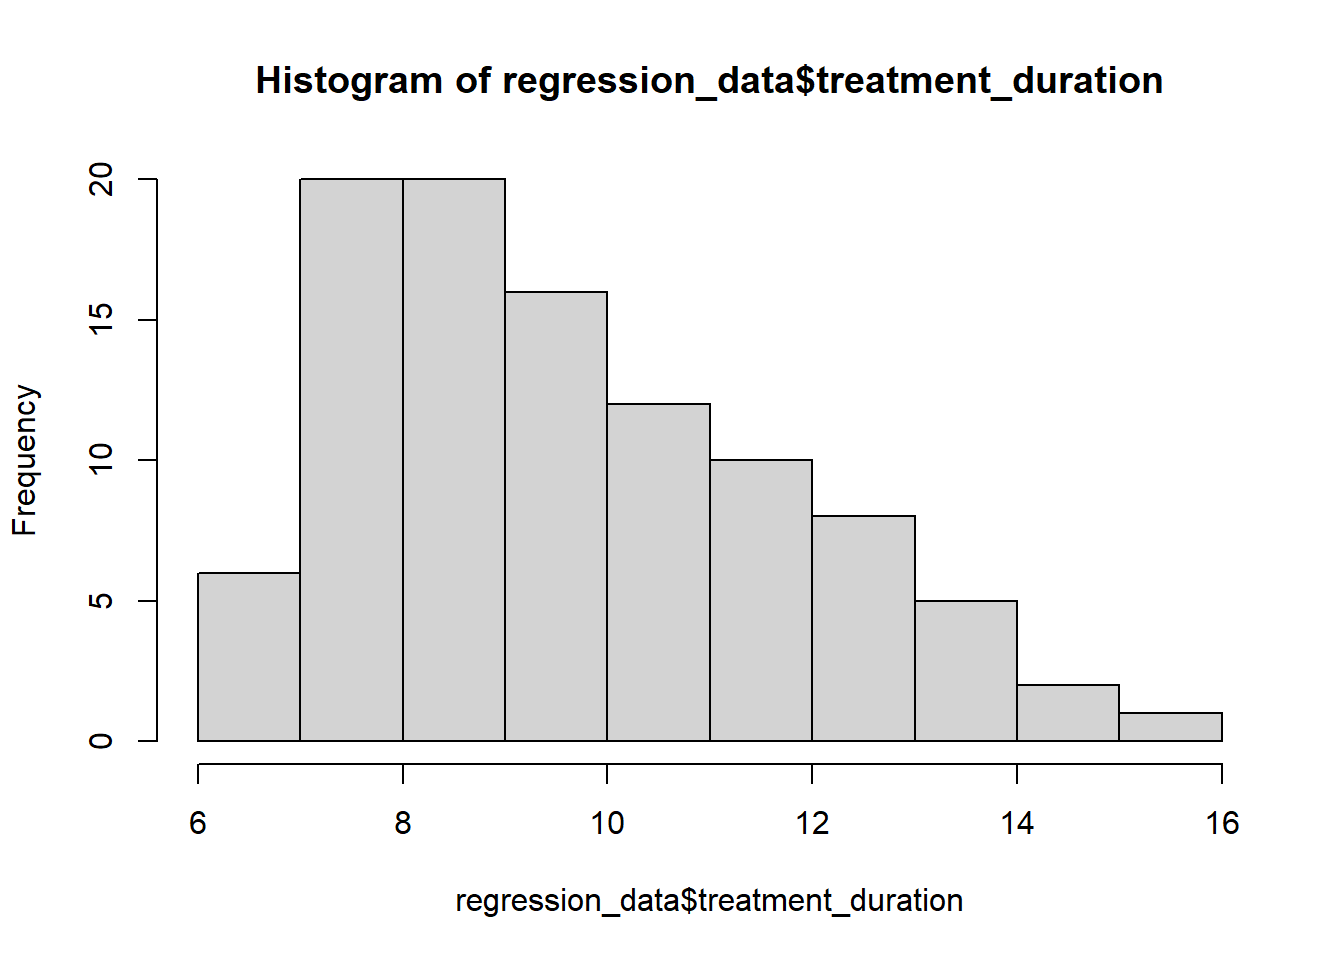
\includegraphics{PRBook_files/figure-latex/unnamed-chunk-61-1} \end{center}

\begin{center}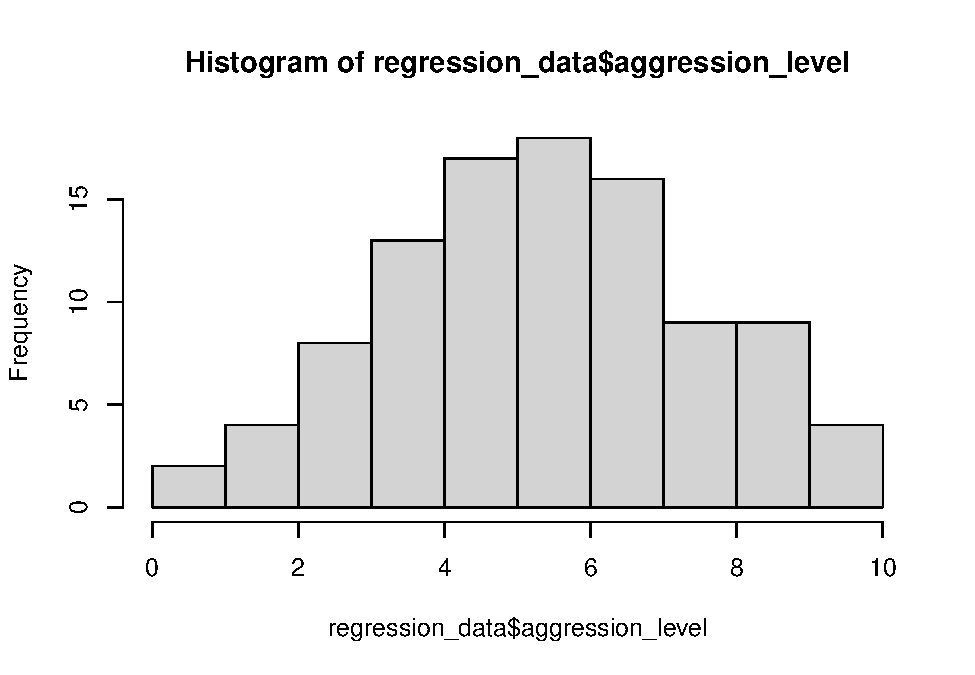
\includegraphics{PRBook_files/figure-latex/unnamed-chunk-62-1} \end{center}

\hypertarget{check-assumptions-distribution-2}{%
\subsection{Check assumptions: distribution \#2}\label{check-assumptions-distribution-2}}

\begin{itemize}
\tightlist
\item
  Parametric tests require normally distributed data
\end{itemize}

\begin{Shaded}
\begin{Highlighting}[]
\KeywordTok{shapiro.test}\NormalTok{(regression_data}\OperatorTok{$}\NormalTok{treatment_duration)}
\end{Highlighting}
\end{Shaded}

\begin{verbatim}
## 
##  Shapiro-Wilk normality test
## 
## data:  regression_data$treatment_duration
## W = 0.94971, p-value = 0.0007939
\end{verbatim}

\begin{Shaded}
\begin{Highlighting}[]
\KeywordTok{shapiro.test}\NormalTok{(regression_data}\OperatorTok{$}\NormalTok{aggression_level)}
\end{Highlighting}
\end{Shaded}

\begin{verbatim}
## 
##  Shapiro-Wilk normality test
## 
## data:  regression_data$aggression_level
## W = 0.9928, p-value = 0.8756
\end{verbatim}

\begin{itemize}
\tightlist
\item
  The normality assumption is less of an issue when sample size is \textgreater{} 30
\end{itemize}

\hypertarget{checking-assumptions-linearity}{%
\subsection{Checking assumptions: linearity}\label{checking-assumptions-linearity}}

\begin{center}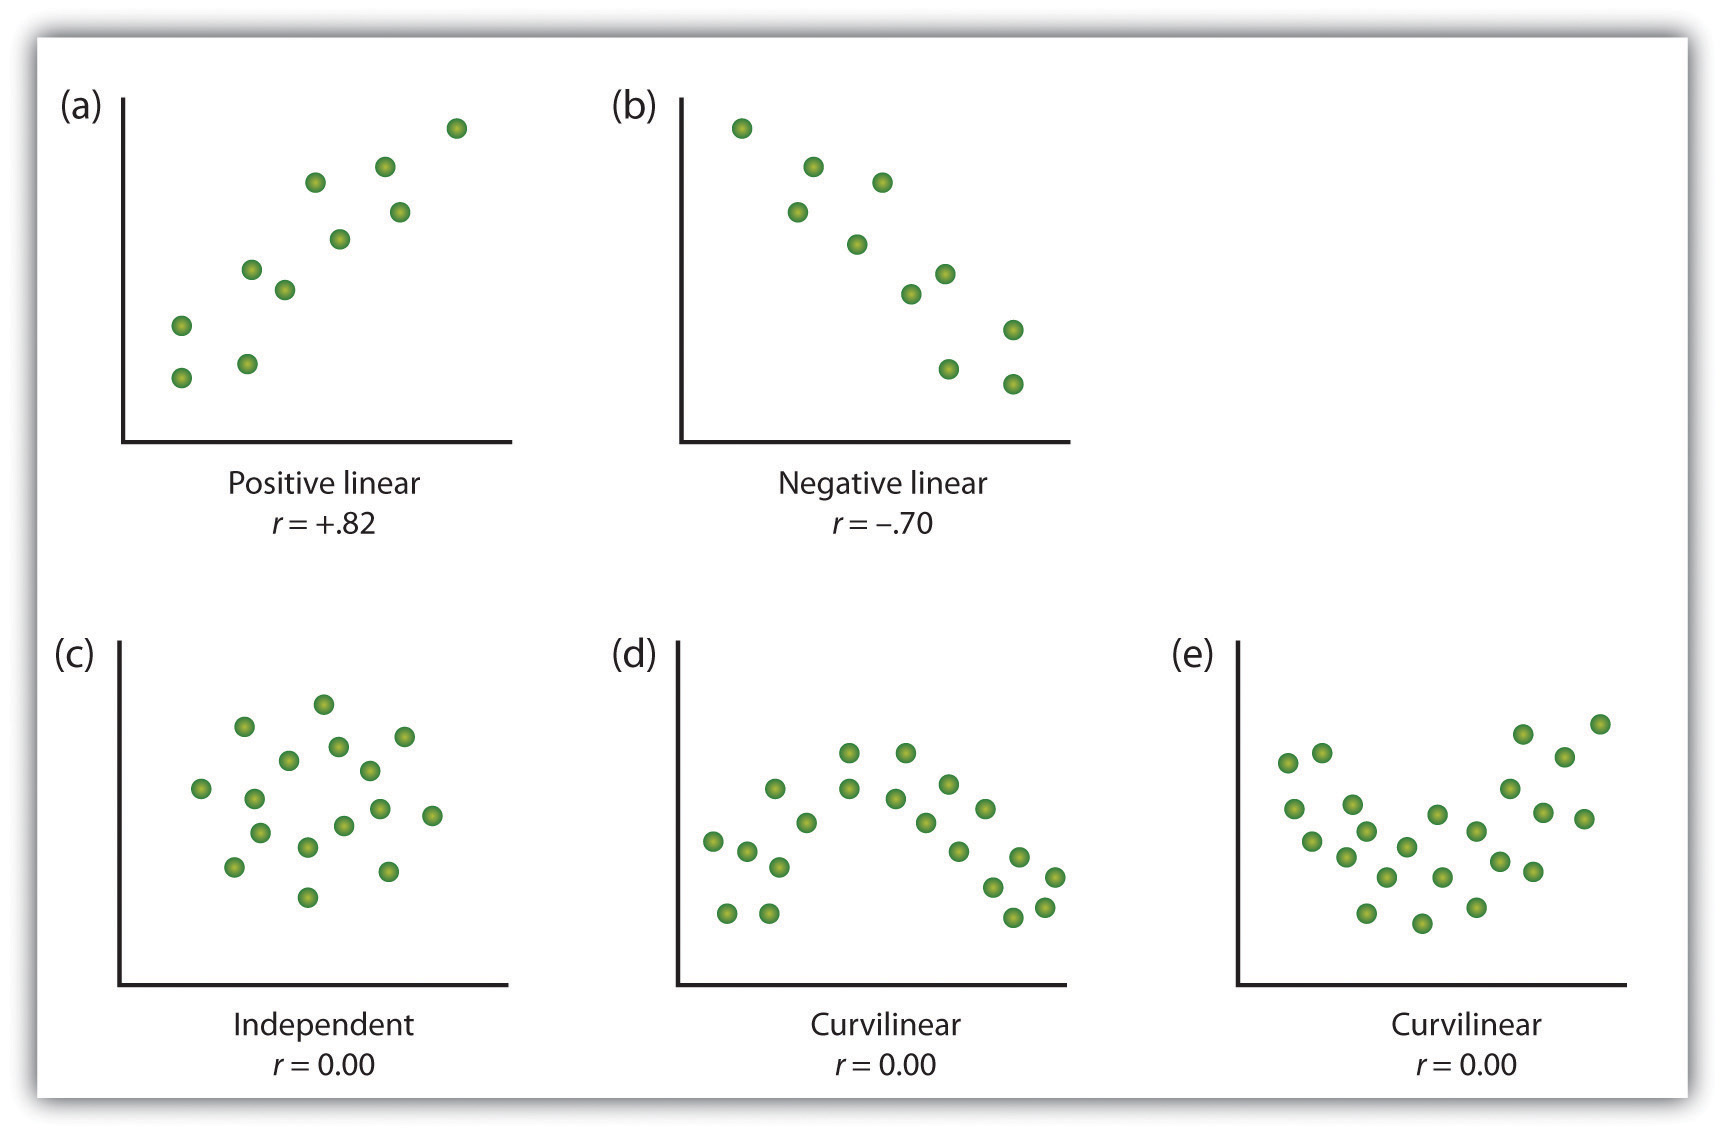
\includegraphics[width=23.97in]{img/curvilinear} \end{center}

\begin{Shaded}
\begin{Highlighting}[]
\NormalTok{regression_data }\OperatorTok\StringTok{ }\KeywordTok{ggplot}\NormalTok{(}\KeywordTok{aes}\NormalTok{(}\DataTypeTok{x=}\NormalTok{treatment_duration,}\DataTypeTok{y=}\NormalTok{aggression_level)) }\OperatorTok{+}
\StringTok{  }\KeywordTok{geom_point}\NormalTok{()}
\end{Highlighting}
\end{Shaded}

\begin{center}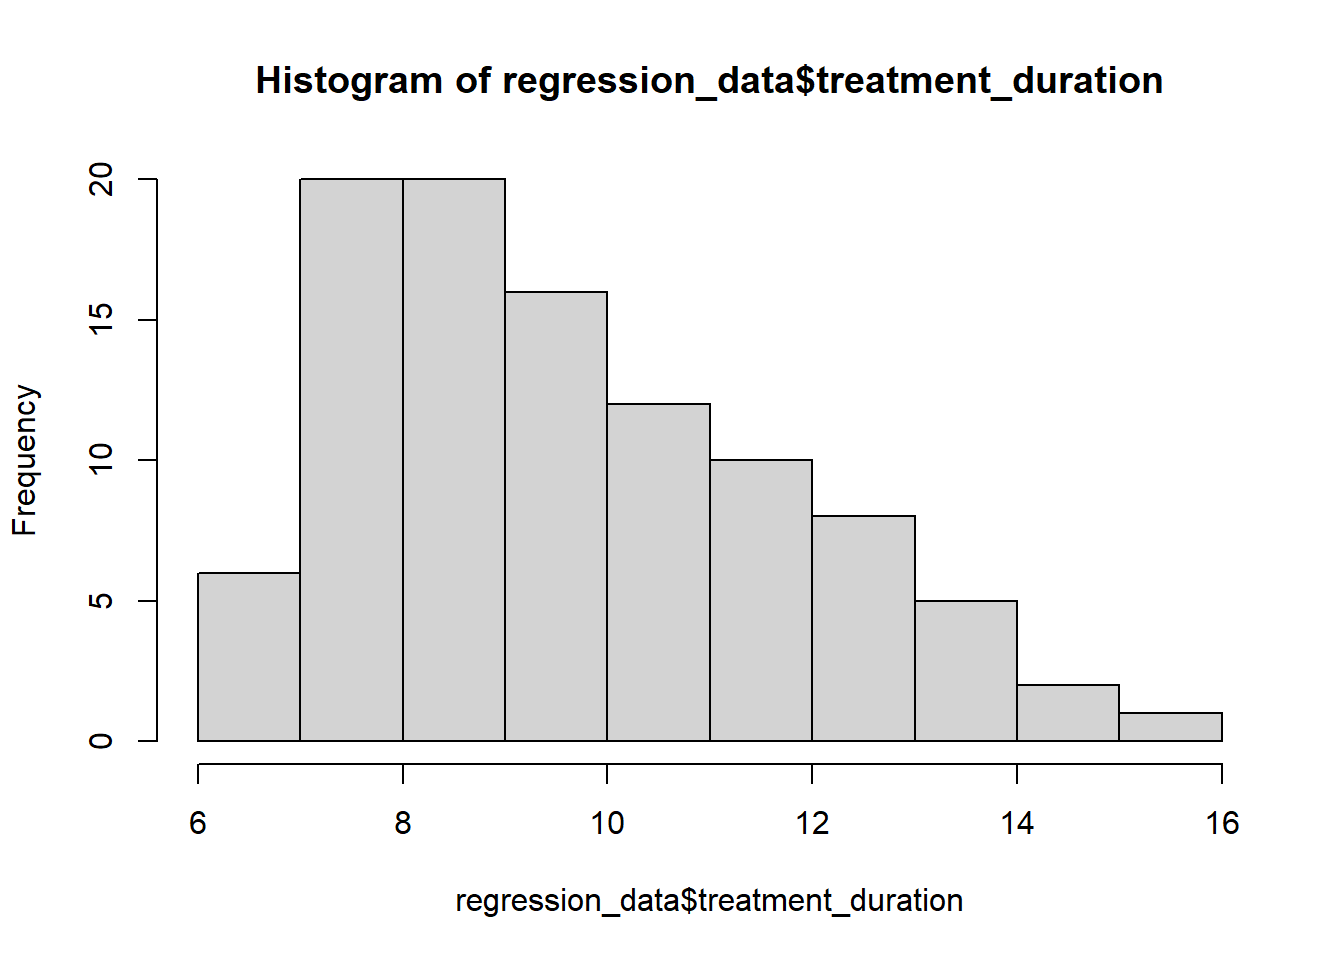
\includegraphics{PRBook_files/figure-latex/unnamed-chunk-66-1} \end{center}

\begin{itemize}
\tightlist
\item
  Here we are looking to see if the relationship is linear
\end{itemize}

\hypertarget{run-correlation}{%
\subsection{Run correlation}\label{run-correlation}}

\begin{itemize}
\tightlist
\item
  R can run correlations using the \emph{cor.test()} command
\end{itemize}

\begin{Shaded}
\begin{Highlighting}[]
\KeywordTok{cor.test}\NormalTok{(regression_data}\OperatorTok{$}\NormalTok{treatment_duration,regression_data}\OperatorTok{$}\NormalTok{aggression_level)}
\end{Highlighting}
\end{Shaded}

\begin{verbatim}
## 
##  Pearson's product-moment correlation
## 
## data:  regression_data$treatment_duration and regression_data$aggression_level
## t = -9.5503, df = 98, p-value = 1.146e-15
## alternative hypothesis: true correlation is not equal to 0
## 95 percent confidence interval:
##  -0.7838251 -0.5765006
## sample estimates:
##        cor 
## -0.6942996
\end{verbatim}

\hypertarget{check-r-value-correlation-value}{%
\subsection{Check r Value (correlation value)}\label{check-r-value-correlation-value}}

\begin{itemize}
\tightlist
\item
  The r value tells us the strength and direction of the relationship
\item
  In the output it is labelled as ``cor'' (short for correlation)
\end{itemize}

\begin{Shaded}
\begin{Highlighting}[]
\KeywordTok{cor.test}\NormalTok{(regression_data}\OperatorTok{$}\NormalTok{treatment_duration,regression_data}\OperatorTok{$}\NormalTok{aggression_level)}
\end{Highlighting}
\end{Shaded}

\begin{verbatim}
## 
##  Pearson's product-moment correlation
## 
## data:  regression_data$treatment_duration and regression_data$aggression_level
## t = -9.5503, df = 98, p-value = 1.146e-15
## alternative hypothesis: true correlation is not equal to 0
## 95 percent confidence interval:
##  -0.7838251 -0.5765006
## sample estimates:
##        cor 
## -0.6942996
\end{verbatim}

\hypertarget{check-the-significance-of-the-correlation}{%
\subsection{Check the significance of the correlation}\label{check-the-significance-of-the-correlation}}

\begin{itemize}
\tightlist
\item
  We can see that the significance by looking at the p value

  \begin{itemize}
  \tightlist
  \item
    The significance is 1.146\^{}-15
  \item
    This means: 0.0000000000000001146
  \end{itemize}
\item
  Therefore p value \textless{} 0.05
\end{itemize}

\begin{Shaded}
\begin{Highlighting}[]
\KeywordTok{cor.test}\NormalTok{(regression_data}\OperatorTok{$}\NormalTok{treatment_duration,regression_data}\OperatorTok{$}\NormalTok{aggression_level)}
\end{Highlighting}
\end{Shaded}

\begin{verbatim}
## 
##  Pearson's product-moment correlation
## 
## data:  regression_data$treatment_duration and regression_data$aggression_level
## t = -9.5503, df = 98, p-value = 1.146e-15
## alternative hypothesis: true correlation is not equal to 0
## 95 percent confidence interval:
##  -0.7838251 -0.5765006
## sample estimates:
##        cor 
## -0.6942996
\end{verbatim}

\hypertarget{simple-regression}{%
\chapter{Simple Regression}\label{simple-regression}}

\hypertarget{what-is-regression}{%
\section{What is regression?}\label{what-is-regression}}

\begin{itemize}
\tightlist
\item
  Testing to see if we can make predictions based on data that are correlated
\end{itemize}

\begin{quote}
We found a strong correlation between treatment duration and agression levels. Can we use this data to predict aggression levels of other clients, based on their treatment duration?
\end{quote}

\begin{itemize}
\tightlist
\item
  When we carry out regression, we get a information about:

  \begin{itemize}
  \tightlist
  \item
    How much variance in the \textbf{outcome} is explained by the \textbf{predictor}
  \item
    How confident we can be about these results generalising (i.e.~\textbf{significance})
  \item
    How much error we can expect from anu predictions that we make (i.e.~\textbf{standard error of the estimate})
  \item
    The figures we need to calculate a predicted outcome value (i.e.~\textbf{coefficient values})
  \end{itemize}
\end{itemize}

\hypertarget{how-is-regression-calculated}{%
\section{How is regression calculated?}\label{how-is-regression-calculated}}

\begin{center}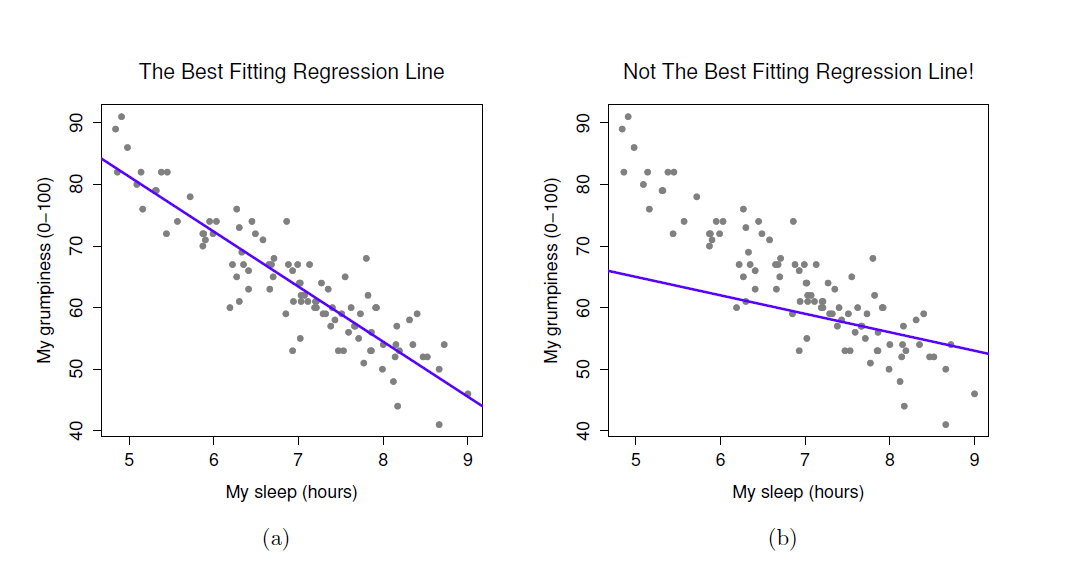
\includegraphics[width=14.88in]{img/bestfit} \end{center}

\begin{itemize}
\tightlist
\item
  When we run a regression analysis, a calculation is done to select the ``line of best fit''
\item
  This is a ``prediction line'' that minimises the overall amount of error

  \begin{itemize}
  \tightlist
  \item
    Error = difference between the data points and the line
  \end{itemize}
\end{itemize}

\hypertarget{the-regression-equation}{%
\section{The regression equation}\label{the-regression-equation}}

\begin{center}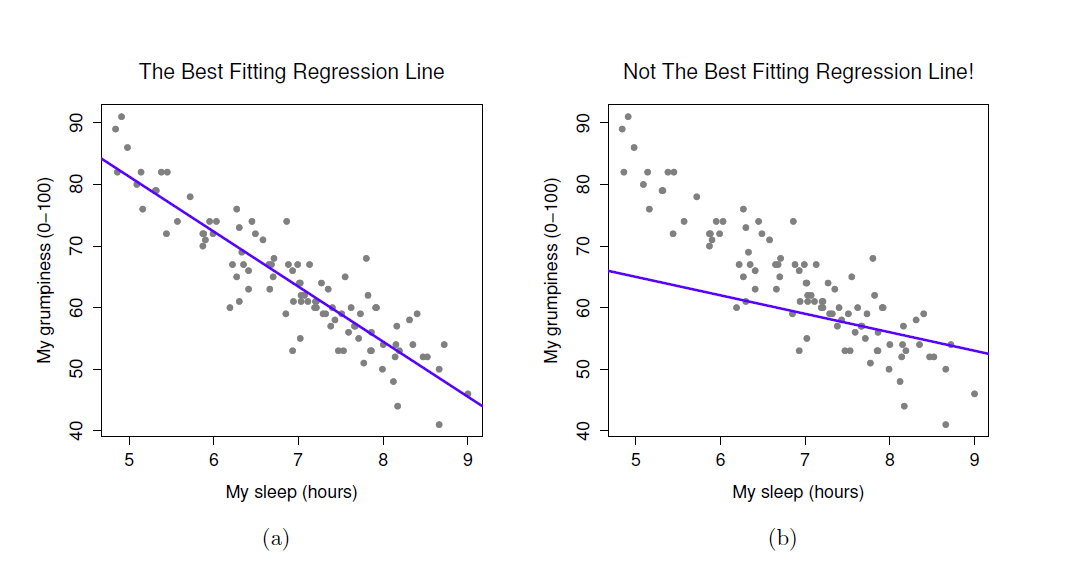
\includegraphics[width=14.88in]{img/bestfit} \end{center}

\begin{itemize}
\item
  Once the line of best fit is calculated, predictions are based on this line
\item
  To make predictions we need the \textbf{intercept} and \textbf{slope} of the line

  \begin{itemize}
  \tightlist
  \item
    \textbf{Intercept} or \textbf{constant}= where the line crosses the y axis
  \item
    \textbf{Slope} or \textbf{beta} = the angle of the line
  \end{itemize}
\item
  Predictions are made using the calculation for a line:
  \textbf{Y = bX + c}
\item
  You can think of the equation like this:
\end{itemize}

\textbf{predicted outcome value = beta coefficient * value of predictor + constant }

\hypertarget{running-regression-in-r}{%
\section{Running regression in R}\label{running-regression-in-r}}

\begin{itemize}
\tightlist
\item
  Step 1: Run regression
\item
  Step 2: Check assumptions

  \begin{itemize}
  \tightlist
  \item
    Data
  \item
    Distribution
  \item
    Linearity
  \item
    Homogeneity of variance
  \item
    Uncorrelated predictors
  \item
    Indpendence of residuals
  \item
    No influental cases / outliers
  \end{itemize}
\item
  Step 3: Check R\^{}2 value
\item
  Step 4: Check model significance
\item
  Step 5: Check coefficient values
\end{itemize}

\hypertarget{run-regression}{%
\section{Run regression}\label{run-regression}}

\begin{itemize}
\tightlist
\item
  We use the \emph{lm()} command to run regression while saving the results
\item
  We then use the \emph{summary()} function to check the results
\end{itemize}

\begin{Shaded}
\begin{Highlighting}[]
\NormalTok{model1 <-}\StringTok{ }\KeywordTok{lm}\NormalTok{(}\DataTypeTok{formula=}\NormalTok{ aggression_level }\OperatorTok{~}\StringTok{ }\NormalTok{treatment_duration ,}\DataTypeTok{data=}\NormalTok{regression_data)}
\KeywordTok{summary}\NormalTok{(model1)}
\end{Highlighting}
\end{Shaded}

\begin{verbatim}
## 
## Call:
## lm(formula = aggression_level ~ treatment_duration, data = regression_data)
## 
## Residuals:
##     Min      1Q  Median      3Q     Max 
## -3.4251 -1.1493 -0.0593  0.8814  3.4542 
## 
## Coefficients:
##                    Estimate Std. Error t value Pr(>|t|)    
## (Intercept)         12.3300     0.7509   16.42  < 2e-16 ***
## treatment_duration  -0.6933     0.0726   -9.55 1.15e-15 ***
## ---
## Signif. codes:  0 '***' 0.001 '**' 0.01 '*' 0.05 '.' 0.1 ' ' 1
## 
## Residual standard error: 1.551 on 98 degrees of freedom
## Multiple R-squared:  0.4821, Adjusted R-squared:  0.4768 
## F-statistic: 91.21 on 1 and 98 DF,  p-value: 1.146e-15
\end{verbatim}

\hypertarget{what-are-residuals}{%
\section{What are residuals?}\label{what-are-residuals}}

\begin{itemize}
\tightlist
\item
  In regression, the assumptions apply to the residuals, not the data themselves
\item
  Residual just means the difference between the data point and the regression line
\end{itemize}

\begin{center}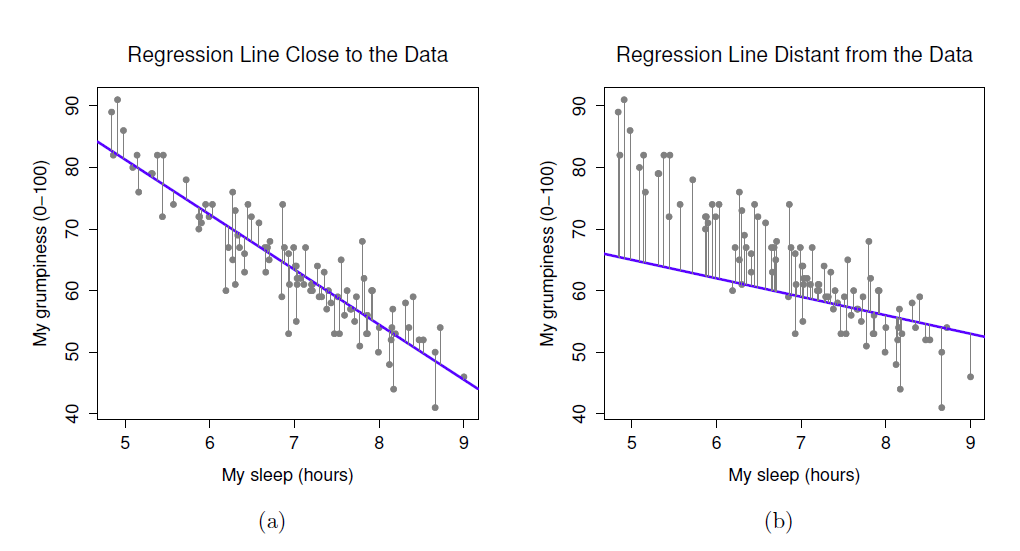
\includegraphics[width=14.17in]{img/residuals1} \end{center}

\hypertarget{check-assumptions-distribution-1}{%
\section{Check assumptions: distribution}\label{check-assumptions-distribution-1}}

\begin{itemize}
\tightlist
\item
  Using the \emph{plot()} command on our regression model will give us some useful diagnostic plots
\item
  The second plot that it outputs shows the normality
\end{itemize}

\begin{Shaded}
\begin{Highlighting}[]
\KeywordTok{plot}\NormalTok{(model1, }\DataTypeTok{which=}\DecValTok{2}\NormalTok{)}
\end{Highlighting}
\end{Shaded}

\begin{center}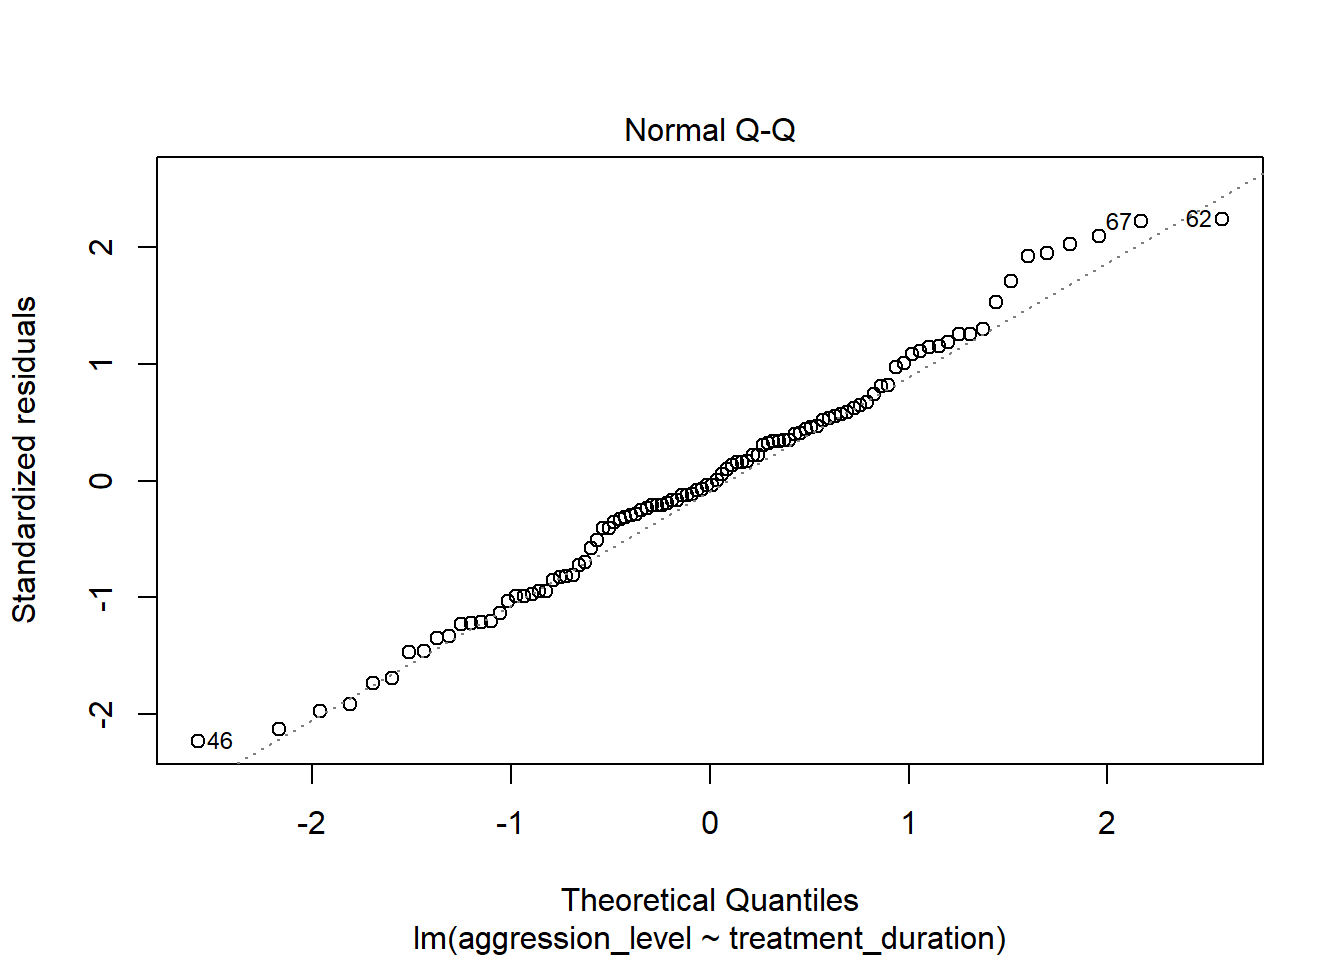
\includegraphics{PRBook_files/figure-latex/unnamed-chunk-74-1} \end{center}

\begin{itemize}
\tightlist
\item
  We could also use a histogram to check the distribution
\item
  Notice how we can use the \$ sign to get the residuals from the model
\end{itemize}

\begin{Shaded}
\begin{Highlighting}[]
\KeywordTok{hist}\NormalTok{(model1}\OperatorTok{$}\NormalTok{residuals)}
\end{Highlighting}
\end{Shaded}

\begin{center}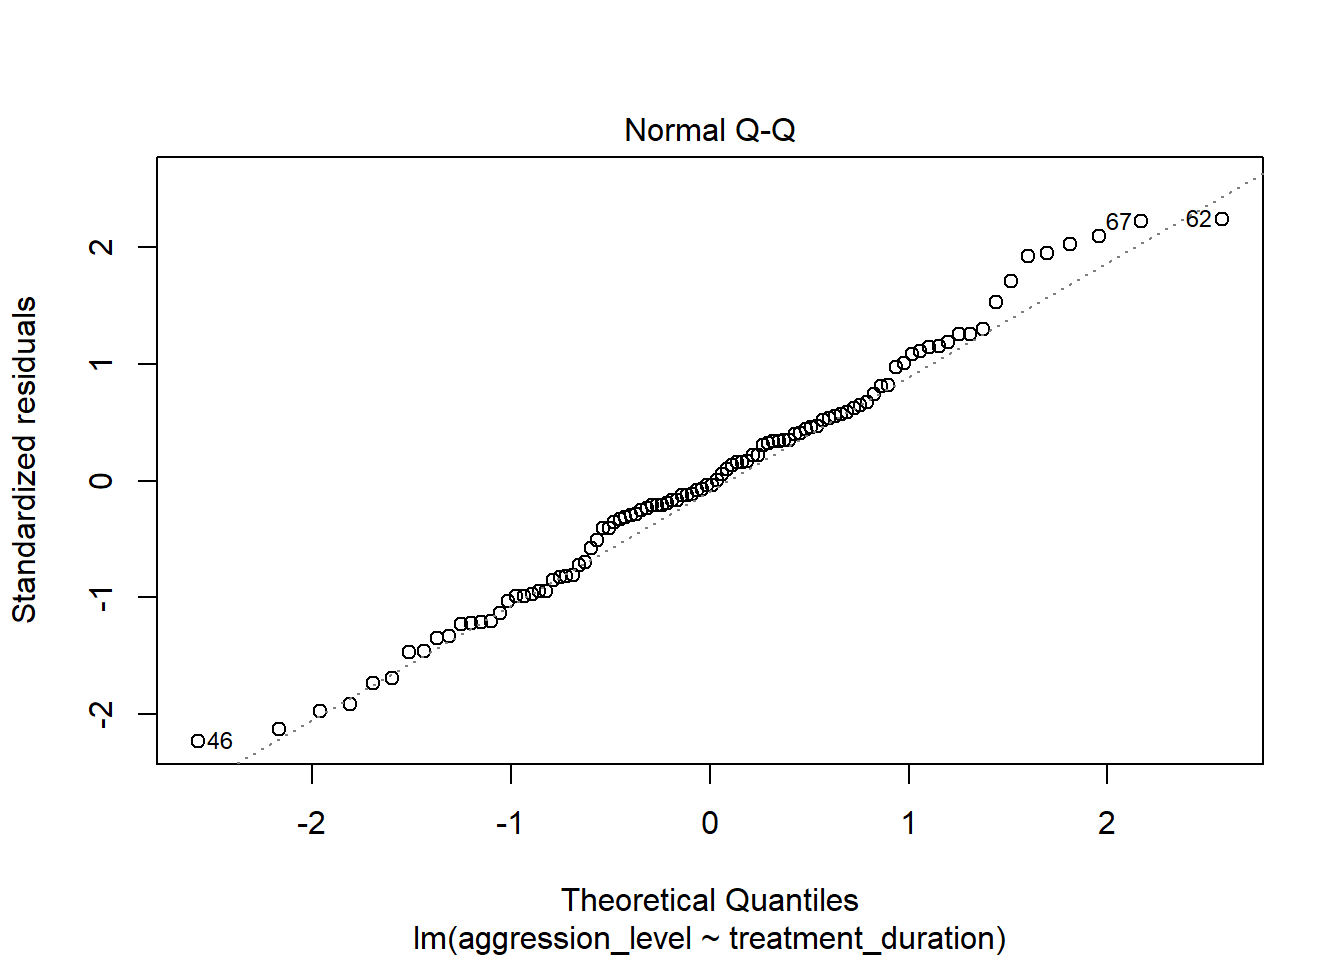
\includegraphics{PRBook_files/figure-latex/unnamed-chunk-75-1} \end{center}

\hypertarget{check-assumptions-linearity}{%
\section{Check assumptions: linearity}\label{check-assumptions-linearity}}

\begin{itemize}
\tightlist
\item
  Using the \emph{plot()} command on our regression model will give us some useful diagnostic plots
\item
  The first plot that it outputs shows the residuals vs the fitted values
\item
  Here, we want to see them spread out, with the line being horizontal and straight
\end{itemize}

\begin{Shaded}
\begin{Highlighting}[]
\KeywordTok{plot}\NormalTok{(model1, }\DataTypeTok{which=}\DecValTok{1}\NormalTok{)}
\end{Highlighting}
\end{Shaded}

\begin{center}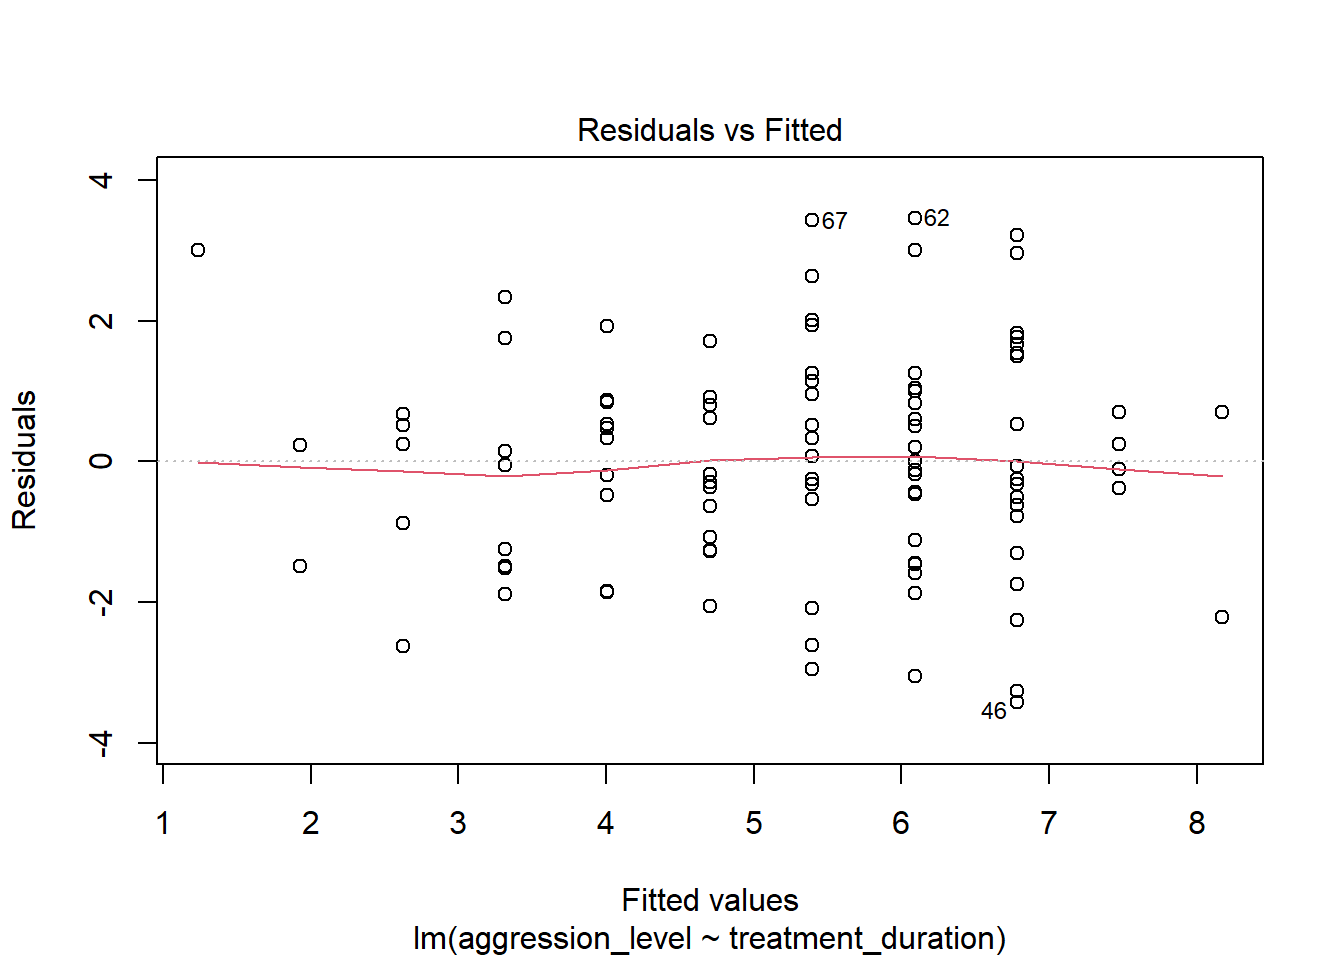
\includegraphics{PRBook_files/figure-latex/unnamed-chunk-76-1} \end{center}

\begin{itemize}
\tightlist
\item
  There is a slight amount of curvilinearity here but nothing to be worried about
\end{itemize}

\hypertarget{check-assumptions-homogeneity-of-variance-1}{%
\section{Check assumptions: Homogeneity of Variance \#1}\label{check-assumptions-homogeneity-of-variance-1}}

\begin{itemize}
\tightlist
\item
  We can use the sample plot to check Homogeneity of Variance
\item
  We want the variance to be constant across the data set. We do not want the variance to change at different points in the data
\end{itemize}

\begin{Shaded}
\begin{Highlighting}[]
\KeywordTok{plot}\NormalTok{(model1, }\DataTypeTok{which=}\DecValTok{1}\NormalTok{)}
\end{Highlighting}
\end{Shaded}

\begin{center}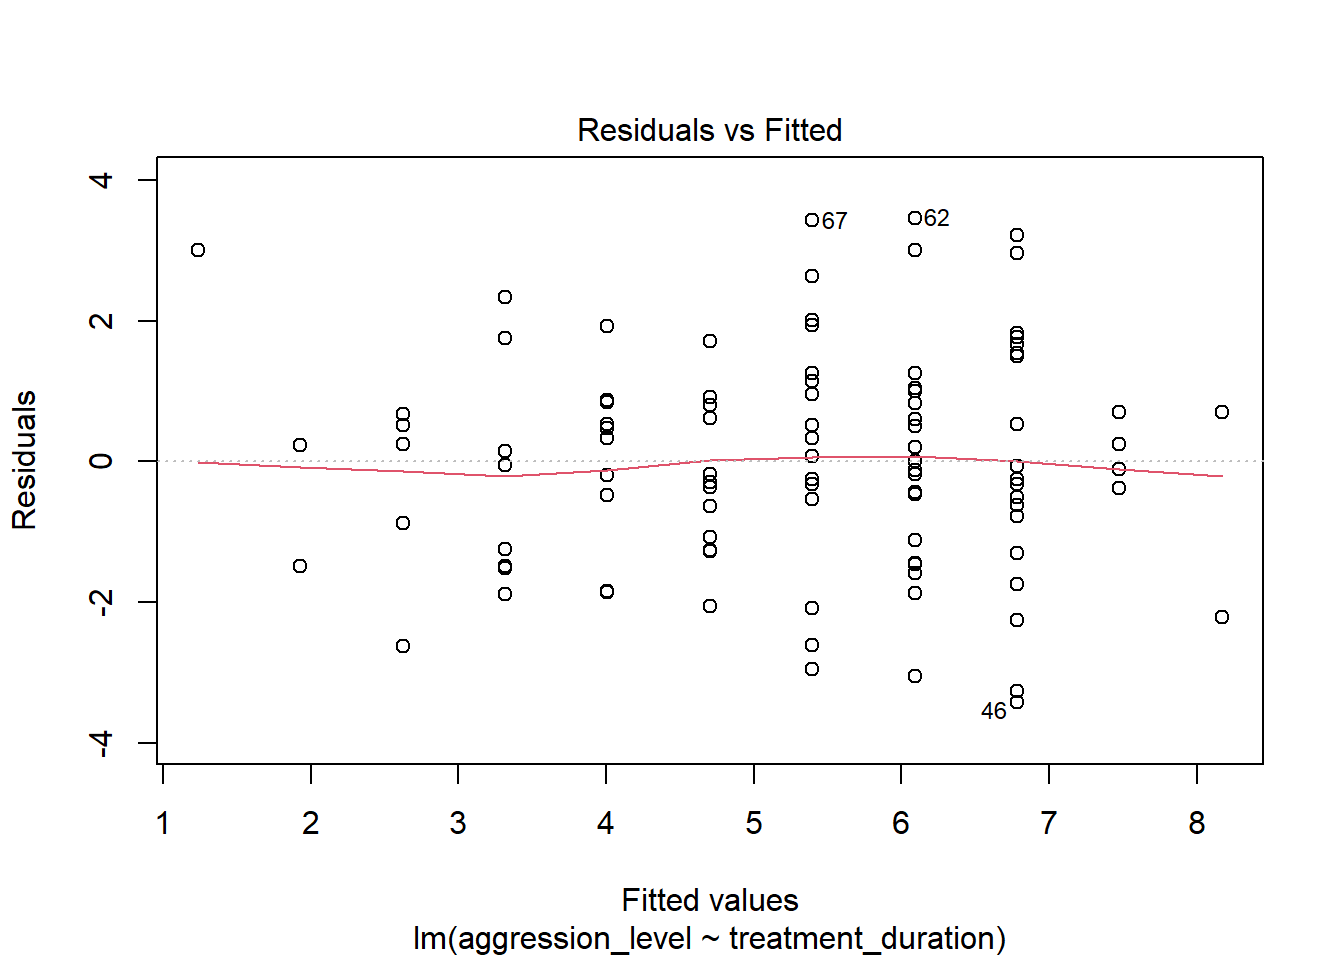
\includegraphics{PRBook_files/figure-latex/unnamed-chunk-77-1} \end{center}

\begin{itemize}
\tightlist
\item
  A violation of Homogeneity of Variance would usually look like a funnel, with the data narrowing
\end{itemize}

\begin{center}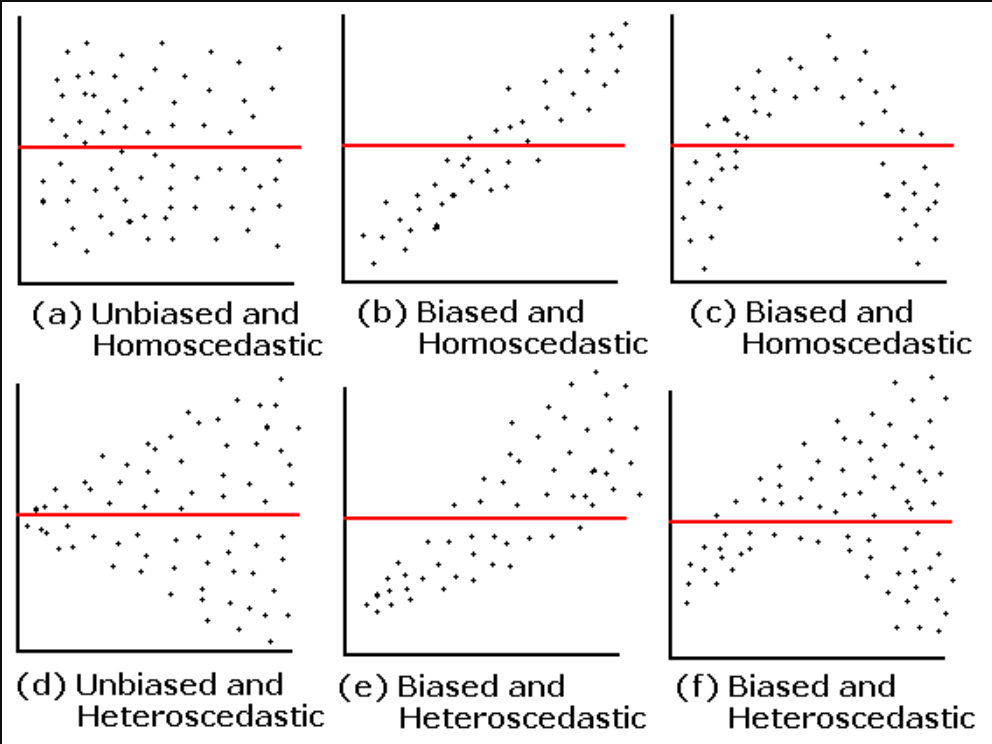
\includegraphics[width=13.78in,height=1\textheight]{img/biasedresiduals} \end{center}

\hypertarget{check-assumptions-influential-cases}{%
\section{Check assumptions: Influential cases}\label{check-assumptions-influential-cases}}

\begin{itemize}
\tightlist
\item
  We need to check that there are no extreme outliers - they could throw off our predictions
\item
  We are looking for participants that have high rediduals + high leverage

  \begin{itemize}
  \tightlist
  \item
    Some guidance suggests anything higher than 1 is an influential case
  \item
    Others suggest 4/n is the cut off point (4 divided by number of participants)
  \end{itemize}
\end{itemize}

\begin{Shaded}
\begin{Highlighting}[]
\KeywordTok{plot}\NormalTok{(model1, }\DataTypeTok{which=}\DecValTok{4}\NormalTok{)}
\end{Highlighting}
\end{Shaded}

\begin{center}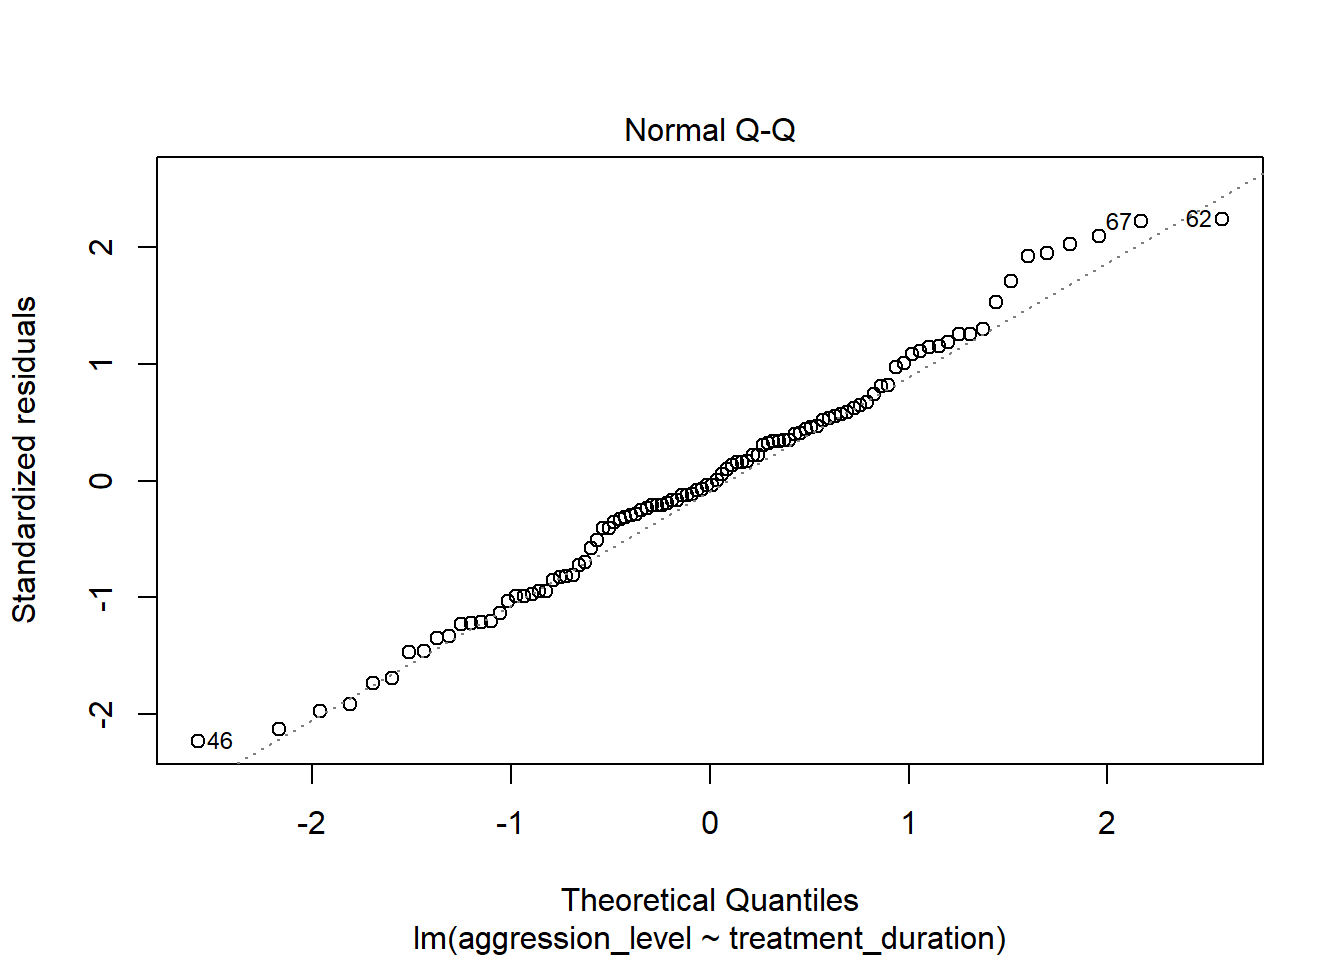
\includegraphics[width=0.3\linewidth]{PRBook_files/figure-latex/unnamed-chunk-79-1} \end{center}

\begin{itemize}
\tightlist
\item
  We are looking for participants that have high rediduals + high leverage

  \begin{itemize}
  \tightlist
  \item
    No cases over 1
  \item
    Many are over 0.04 (4/n = 0.04)
  \end{itemize}
\end{itemize}

\begin{Shaded}
\begin{Highlighting}[]
\KeywordTok{plot}\NormalTok{(model1, }\DataTypeTok{which=}\DecValTok{5}\NormalTok{)}
\end{Highlighting}
\end{Shaded}

\begin{center}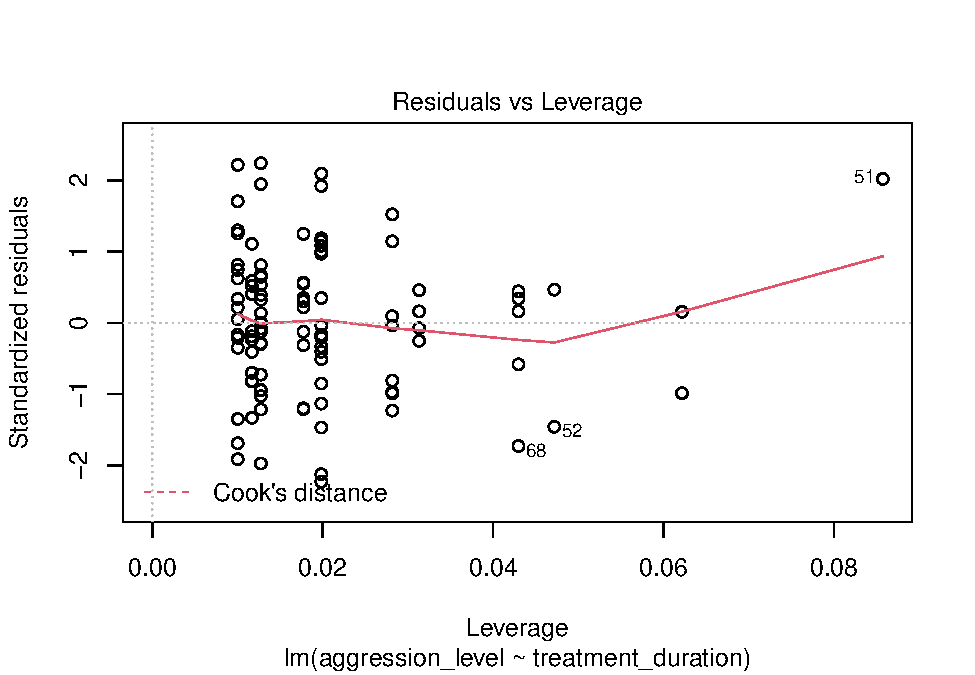
\includegraphics[width=0.4\linewidth]{PRBook_files/figure-latex/unnamed-chunk-80-1} \end{center}

\hypertarget{check-the-r-squared-value}{%
\section{Check the r squared value}\label{check-the-r-squared-value}}

\begin{itemize}
\tightlist
\item
  r\^{}2 = the amount of variance in the \textbf{outcome} that is explained by the \textbf{predictor(s)}
\item
  The closer this value is to 1, the more useful our regression model is for predicting the outcome
\end{itemize}

\begin{Shaded}
\begin{Highlighting}[]
\NormalTok{modelSummary <-}\StringTok{ }\KeywordTok{summary}\NormalTok{(model1)}
\NormalTok{modelSummary}
\end{Highlighting}
\end{Shaded}

\begin{verbatim}
## 
## Call:
## lm(formula = aggression_level ~ treatment_duration, data = regression_data)
## 
## Residuals:
##     Min      1Q  Median      3Q     Max 
## -3.4251 -1.1493 -0.0593  0.8814  3.4542 
## 
## Coefficients:
##                    Estimate Std. Error t value Pr(>|t|)    
## (Intercept)         12.3300     0.7509   16.42  < 2e-16 ***
## treatment_duration  -0.6933     0.0726   -9.55 1.15e-15 ***
## ---
## Signif. codes:  0 '***' 0.001 '**' 0.01 '*' 0.05 '.' 0.1 ' ' 1
## 
## Residual standard error: 1.551 on 98 degrees of freedom
## Multiple R-squared:  0.4821, Adjusted R-squared:  0.4768 
## F-statistic: 91.21 on 1 and 98 DF,  p-value: 1.146e-15
\end{verbatim}

\begin{itemize}
\tightlist
\item
  The r\^{}2 of 0.482052 means that 48\% of the variance in \textbf{aggression level} is explained by \textbf{treatment duration}
\end{itemize}

\hypertarget{check-model-significance}{%
\section{Check model significance}\label{check-model-significance}}

\begin{itemize}
\tightlist
\item
  The model significance is displayed at the very end of the output

  \begin{itemize}
  \tightlist
  \item
    \emph{p-value: 1.146e-15}
  \item
    As p \textless{} 0.05, the model is significant
  \end{itemize}
\end{itemize}

\begin{Shaded}
\begin{Highlighting}[]
\NormalTok{modelSummary}
\end{Highlighting}
\end{Shaded}

\begin{verbatim}
## 
## Call:
## lm(formula = aggression_level ~ treatment_duration, data = regression_data)
## 
## Residuals:
##     Min      1Q  Median      3Q     Max 
## -3.4251 -1.1493 -0.0593  0.8814  3.4542 
## 
## Coefficients:
##                    Estimate Std. Error t value Pr(>|t|)    
## (Intercept)         12.3300     0.7509   16.42  < 2e-16 ***
## treatment_duration  -0.6933     0.0726   -9.55 1.15e-15 ***
## ---
## Signif. codes:  0 '***' 0.001 '**' 0.01 '*' 0.05 '.' 0.1 ' ' 1
## 
## Residual standard error: 1.551 on 98 degrees of freedom
## Multiple R-squared:  0.4821, Adjusted R-squared:  0.4768 
## F-statistic: 91.21 on 1 and 98 DF,  p-value: 1.146e-15
\end{verbatim}

\hypertarget{check-coefficient-values}{%
\section{Check coefficient values}\label{check-coefficient-values}}

\begin{itemize}
\tightlist
\item
  The coefficient values are displayed in the coefficients table
\item
  If we have more than one predictor, they are all listed here
\end{itemize}

\begin{Shaded}
\begin{Highlighting}[]
\NormalTok{modelSummary}\OperatorTok{$}\NormalTok{coefficients}
\end{Highlighting}
\end{Shaded}

\begin{verbatim}
##                      Estimate Std. Error   t value     Pr(>|t|)
## (Intercept)        12.3300211 0.75087601 16.420848 6.840516e-30
## treatment_duration -0.6933201 0.07259671 -9.550297 1.145898e-15
\end{verbatim}

\begin{itemize}
\tightlist
\item
  The \textbf{beta coefficient} for treatment duration is in the \emph{Estimate} column
\item
  For every unit increase in treatment duration, aggression level decreases by 0.69
\end{itemize}

\hypertarget{the-regression-equation-1}{%
\section{The regression equation}\label{the-regression-equation-1}}

\begin{itemize}
\tightlist
\item
  The regression equation is:
\end{itemize}

Outcome = predictor value * beta coefficient + constant

\begin{itemize}
\tightlist
\item
  For this model, that is:
\end{itemize}

Aggression level = treatment duration * -0.69 + 12.33

\begin{Shaded}
\begin{Highlighting}[]
\NormalTok{modelSummary}\OperatorTok{$}\NormalTok{coefficients}
\end{Highlighting}
\end{Shaded}

\begin{verbatim}
##                      Estimate Std. Error   t value     Pr(>|t|)
## (Intercept)        12.3300211 0.75087601 16.420848 6.840516e-30
## treatment_duration -0.6933201 0.07259671 -9.550297 1.145898e-15
\end{verbatim}

\hypertarget{accounting-for-error-in-predictions}{%
\section{Accounting for error in predictions}\label{accounting-for-error-in-predictions}}

\begin{itemize}
\tightlist
\item
  We also know that the accuracy of predictions will be within a certain margin of error
\item
  This is known as \textbf{standard error of the estimate} or \textbf{residual standard error}
\end{itemize}

\begin{Shaded}
\begin{Highlighting}[]
\NormalTok{modelSummary}
\end{Highlighting}
\end{Shaded}

\begin{verbatim}
## 
## Call:
## lm(formula = aggression_level ~ treatment_duration, data = regression_data)
## 
## Residuals:
##     Min      1Q  Median      3Q     Max 
## -3.4251 -1.1493 -0.0593  0.8814  3.4542 
## 
## Coefficients:
##                    Estimate Std. Error t value Pr(>|t|)    
## (Intercept)         12.3300     0.7509   16.42  < 2e-16 ***
## treatment_duration  -0.6933     0.0726   -9.55 1.15e-15 ***
## ---
## Signif. codes:  0 '***' 0.001 '**' 0.01 '*' 0.05 '.' 0.1 ' ' 1
## 
## Residual standard error: 1.551 on 98 degrees of freedom
## Multiple R-squared:  0.4821, Adjusted R-squared:  0.4768 
## F-statistic: 91.21 on 1 and 98 DF,  p-value: 1.146e-15
\end{verbatim}

\hypertarget{multiple-regression}{%
\chapter{Multiple Regression}\label{multiple-regression}}

\hypertarget{by-the-end-of-this-session-you-will-be-able-to}{%
\section{By the end of this session, you will be able to:}\label{by-the-end-of-this-session-you-will-be-able-to}}

\begin{itemize}
\tightlist
\item
  Compare multiple regression to simple regression
\item
  Describe the assumptions of multiple regression
\item
  Consider sample size in regression
\item
  Use categorical predictors in regression in R
\item
  Conduct different types of multiple regression
\item
  Interpret the output of Multiple regression
\end{itemize}

\hypertarget{what-is-multiple-regression}{%
\section{What is multiple regression?}\label{what-is-multiple-regression}}

\begin{itemize}
\tightlist
\item
  An extension of simple regression
\item
  Same format as simple regression but adding each predictor:
\end{itemize}

\[ Y = b_1X_1 + b_2X_2 + b_0 \]

(The constant can be referred to in the equation as \textbf{c} or \textbf{b0} )

\hypertarget{what-are-the-assumptions-of-multiple-regression}{%
\section{What are the assumptions of Multiple Regression?}\label{what-are-the-assumptions-of-multiple-regression}}

\begin{itemize}
\tightlist
\item
  They are primarily the same as simple regression
\item
  The additional assumption of no \textbf{multicollinearity} (due to having multiple predictors)

  \begin{itemize}
  \tightlist
  \item
    i.e.~predictors should not be highly correlated
  \end{itemize}
\end{itemize}

\hypertarget{what-is-multicollinearity}{%
\section{What is multicollinearity?}\label{what-is-multicollinearity}}

\begin{itemize}
\tightlist
\item
  Multicollinearity = predictors correlated highly with each other.
\item
  This is not good because:

  \begin{itemize}
  \tightlist
  \item
    It makes it difficult to determine the role of individual predictors
  \item
    Increases the error of the model (higher standard errors)
  \item
    Difficult to identify significant predictors - wider confidence interval
  \end{itemize}
\end{itemize}

\hypertarget{testing-multicollinearity}{%
\section{Testing multicollinearity}\label{testing-multicollinearity}}

\begin{Shaded}
\begin{Highlighting}[]
\CommentTok{## use the mctest package}
\CommentTok{# install.packages(‘mctest’)o}
\KeywordTok{library}\NormalTok{(mctest)}
\end{Highlighting}
\end{Shaded}

\begin{verbatim}
## Warning: package 'mctest' was built under R version 4.0.2
\end{verbatim}

\begin{Shaded}
\begin{Highlighting}[]
\NormalTok{m1 <-}\StringTok{ }\KeywordTok{lm}\NormalTok{(aggression_level }\OperatorTok{~}\StringTok{ }\NormalTok{treatment_group }\OperatorTok{+}\StringTok{ }\NormalTok{treatment_duration }\OperatorTok{+}\StringTok{ }\NormalTok{trust_score, }\DataTypeTok{data=}\NormalTok{regression_data)}

\KeywordTok{mctest}\NormalTok{(m1) }
\end{Highlighting}
\end{Shaded}

\begin{verbatim}
## 
## Call:
## omcdiag(mod = mod, Inter = TRUE, detr = detr, red = red, conf = conf, 
##     theil = theil, cn = cn)
## 
## 
## Overall Multicollinearity Diagnostics
## 
##                        MC Results detection
## Determinant |X'X|:         0.9229         0
## Farrar Chi-Square:         7.7960         0
## Red Indicator:             0.1547         0
## Sum of Lambda Inverse:     3.1728         0
## Theil's Method:           -0.8800         0
## Condition Number:         13.6549         0
## 
## 1 --> COLLINEARITY is detected by the test 
## 0 --> COLLINEARITY is not detected by the test
\end{verbatim}

\begin{itemize}
\item
  The format of \emph{mctest()} is:

  mctest(predictors, outcome)
\item
  In the above example we used the \emph{cbind()} function to bind 3 columns of data together (the predictors)
\end{itemize}

\hypertarget{sample-size-for-multiple-regression}{%
\section{Sample size for multiple regression}\label{sample-size-for-multiple-regression}}

\begin{itemize}
\tightlist
\item
  Is based on the number of predictors
\item
  More predictors = more participants needed
\item
  \textbf{Do a power analysis}
\item
  Loose ``rule of thumb'' = 10-15 participants per predictor
\end{itemize}

\hypertarget{approaches-to-multiple-regression-all-predictors-at-once}{%
\section{Approaches to multiple regression: All predictors at once}\label{approaches-to-multiple-regression-all-predictors-at-once}}

\begin{quote}
Research question: Do a client's treatment duration and treatment group predict aggression level?
\end{quote}

\begin{Shaded}
\begin{Highlighting}[]
\NormalTok{model1 <-}\StringTok{ }\KeywordTok{lm}\NormalTok{(}\DataTypeTok{data =}\NormalTok{ regression_data, aggression_level }\OperatorTok{~}\StringTok{ }\NormalTok{treatment_duration }\OperatorTok{+}\StringTok{ }\NormalTok{treatment_group)}
\end{Highlighting}
\end{Shaded}

\begin{itemize}
\tightlist
\item
  Here we are including all of the predictors at the same time
\item
  Note that we are using a plus sign + between each predictor

  \begin{itemize}
  \tightlist
  \item
    This means that no interactions will be tested
  \end{itemize}
\end{itemize}

\hypertarget{using-categorical-predictors-in-r}{%
\subsection{Using categorical predictors in R}\label{using-categorical-predictors-in-r}}

\begin{itemize}
\tightlist
\item
  Treatment group is a categorical (also called ``nominal'' or ``factor'') variable
\item
  No special ``dummy coding'' is required in R to use categorical predictors in regression
\item
  R will use the first group as the reference category and test whether being in another group shows a significant difference
\item
  R chooses the reference group based on numerical value or alphabetical order
\item
  If you want you can change the reference category or ``force'' it using the relevel function:
\end{itemize}

\begin{Shaded}
\begin{Highlighting}[]
\NormalTok{regression_data}\OperatorTok{$}\NormalTok{treatment_group <-}\StringTok{ }\KeywordTok{relevel}\NormalTok{(regression_data}\OperatorTok{$}\NormalTok{treatment_group, }\DataTypeTok{ref =} \StringTok{"therapy1"}\NormalTok{)}
\end{Highlighting}
\end{Shaded}

\hypertarget{reviewing-the-output}{%
\subsection{Reviewing the output}\label{reviewing-the-output}}

\begin{Shaded}
\begin{Highlighting}[]
\KeywordTok{summary}\NormalTok{(model1)}
\end{Highlighting}
\end{Shaded}

\begin{verbatim}
## 
## Call:
## lm(formula = aggression_level ~ treatment_duration + treatment_group, 
##     data = regression_data)
## 
## Residuals:
##     Min      1Q  Median      3Q     Max 
## -2.9468 -1.1104  0.0205  0.9621  3.4481 
## 
## Coefficients:
##                         Estimate Std. Error t value Pr(>|t|)    
## (Intercept)             11.58713    0.77331  14.984  < 2e-16 ***
## treatment_duration      -0.66024    0.07119  -9.274 4.96e-15 ***
## treatment_grouptherapy2  0.85032    0.30449   2.793   0.0063 ** 
## ---
## Signif. codes:  0 '***' 0.001 '**' 0.01 '*' 0.05 '.' 0.1 ' ' 1
## 
## Residual standard error: 1.5 on 97 degrees of freedom
## Multiple R-squared:  0.5206, Adjusted R-squared:  0.5107 
## F-statistic: 52.67 on 2 and 97 DF,  p-value: 3.267e-16
\end{verbatim}

\begin{itemize}
\tightlist
\item
  Multiple R\^{}2 = Total variance in outcome that is explained by the model
\item
  p-value = Statistical significance of the model
\item
  Coefficients = Contribution of each predictor to the model

  \begin{itemize}
  \tightlist
  \item
    Pr = Significance of the individual predictor
  \item
    Estimate = Change in the outcome level that occurs when the predictor increases by 1 unit of measurement
  \end{itemize}
\end{itemize}

\hypertarget{all-predictors-at-once-testing-interactions}{%
\subsection{All predictors at once (testing interactions)}\label{all-predictors-at-once-testing-interactions}}

\begin{quote}
Research questions:
- Do a client's treatment duration and treatment group predict aggression level
- Do the predictors interact?
\end{quote}

\begin{Shaded}
\begin{Highlighting}[]
\NormalTok{model2 <-}\StringTok{ }\KeywordTok{lm}\NormalTok{(}\DataTypeTok{data =}\NormalTok{ regression_data, aggression_level }\OperatorTok{~}\StringTok{ }\NormalTok{treatment_duration }\OperatorTok{*}\StringTok{ }\NormalTok{treatment_group)}
\end{Highlighting}
\end{Shaded}

\begin{itemize}
\tightlist
\item
  Here we are including all of the predictors at the same time
\item
  Note that we are using an asterisk * between each predictor

  \begin{itemize}
  \tightlist
  \item
    This means that interactions will be tested
  \end{itemize}
\end{itemize}

Reviewing the output

\begin{Shaded}
\begin{Highlighting}[]
\KeywordTok{summary}\NormalTok{(model2) }\OperatorTok\StringTok{ }\NormalTok{coefficients}
\end{Highlighting}
\end{Shaded}

\begin{verbatim}
##                                              Estimate Std. Error    t value
## (Intercept)                                12.3529190  1.1006127 11.2236751
## treatment_duration                         -0.7334435  0.1033086 -7.0995381
## treatment_grouptherapy2                    -0.5615517  1.4753596 -0.3806202
## treatment_duration:treatment_grouptherapy2  0.1394649  0.1425977  0.9780305
##                                                Pr(>|t|)
## (Intercept)                                3.599000e-19
## treatment_duration                         2.166226e-10
## treatment_grouptherapy2                    7.043260e-01
## treatment_duration:treatment_grouptherapy2 3.305175e-01
\end{verbatim}

\begin{itemize}
\tightlist
\item
  We get additional information in the coefficients table about the interaction between variables

  \begin{itemize}
  \tightlist
  \item
    e.g.~does the interaction between level of trust and treatment duration predict the outcome (aggression level)?
  \end{itemize}
\item
  We can see from the output that none of the interactions are significant
\end{itemize}

\hypertarget{hierarchical-multiple-regression-theory-driven-blocks-of-variables}{%
\subsection{Hierarchical multiple regression: Theory driven ``blocks'' of variables}\label{hierarchical-multiple-regression-theory-driven-blocks-of-variables}}

\begin{itemize}
\tightlist
\item
  It might be the case that we have previous research or theory to guide how we run the analysis
\item
  For example, we might know that treatment duration and therapy group are likely to predict the outcome
\item
  We might want to check whether client's level of trust in the clinician has any \textbf{additional} impact on our ability to predict the outcome (aggression level)
\end{itemize}

\begin{quote}
\begin{itemize}
\tightlist
\item
  To do this, we run three regression models

  \begin{itemize}
  \tightlist
  \item
    Model 0: the constant (baseline)
  \item
    Model 1: treatment duration and therapy group
  \item
    Model 2: treatment duration and therapy group and trust score
  \end{itemize}
\end{itemize}
\end{quote}

\begin{itemize}
\tightlist
\item
  We then compare the two regression models to see if:

  \begin{itemize}
  \tightlist
  \item
    Model 1 is better than Model 0 (the constant)
  \item
    Model 2 is better than Model 1
  \end{itemize}
\end{itemize}

\textbf{Hierarchical multiple regression: Running and comparing 2 models}

\begin{Shaded}
\begin{Highlighting}[]
\CommentTok{## run regression using the same method as above}
\NormalTok{model0 <-}\StringTok{ }\KeywordTok{lm}\NormalTok{(}\DataTypeTok{data =}\NormalTok{ regression_data, aggression_level }\OperatorTok{~}\StringTok{ }\DecValTok{1}\NormalTok{)}
\NormalTok{model1 <-}\StringTok{ }\KeywordTok{lm}\NormalTok{(}\DataTypeTok{data =}\NormalTok{ regression_data, aggression_level }\OperatorTok{~}\StringTok{ }\NormalTok{treatment_duration }\OperatorTok{+}\StringTok{ }\NormalTok{treatment_group)}
\NormalTok{model2 <-}\StringTok{ }\KeywordTok{lm}\NormalTok{(}\DataTypeTok{data =}\NormalTok{ regression_data, aggression_level }\OperatorTok{~}\StringTok{ }\NormalTok{treatment_duration }\OperatorTok{+}\StringTok{ }\NormalTok{treatment_group }\OperatorTok{+}\StringTok{ }\NormalTok{trust_score)}

\CommentTok{## use the aov() command to compare the models}
\KeywordTok{anova}\NormalTok{(model0,model1,model2)}
\end{Highlighting}
\end{Shaded}

\begin{verbatim}
## Analysis of Variance Table
## 
## Model 1: aggression_level ~ 1
## Model 2: aggression_level ~ treatment_duration + treatment_group
## Model 3: aggression_level ~ treatment_duration + treatment_group + trust_score
##   Res.Df    RSS Df Sum of Sq       F    Pr(>F)    
## 1     99 455.27                                   
## 2     97 218.26  2   237.013 52.2195 4.507e-16 ***
## 3     96 217.86  1     0.399  0.1757     0.676    
## ---
## Signif. codes:  0 '***' 0.001 '**' 0.01 '*' 0.05 '.' 0.1 ' ' 1
\end{verbatim}

\begin{itemize}
\tightlist
\item
  We can see that:

  \begin{itemize}
  \tightlist
  \item
    Model 1 (treatment duration and treatment group) is significant relative to the constant (Model 0)
  \item
    Model 2 (treatment duration, treatment group and trust score) shows no significant change compared to Model 1
  \end{itemize}
\end{itemize}

\hypertarget{stepwise-multiple-regression-computational-selection-of-predictors}{%
\subsection{Stepwise multiple regression: computational selection of predictors}\label{stepwise-multiple-regression-computational-selection-of-predictors}}

\begin{itemize}
\tightlist
\item
  Stepwise multiple regression is controversial because:

  \begin{itemize}
  \tightlist
  \item
    The computer selects which predictors to include based on Akaike information criterion (AIC)

    \begin{itemize}
    \tightlist
    \item
      This is a calculation of the quality of statistical models when they are compared to each other
    \end{itemize}
  \end{itemize}

  \begin{quote}
  \hypertarget{whats-the-problem}{%
  \subsection{What's the problem?}\label{whats-the-problem}}

  \begin{itemize}
  \tightlist
  \item
    This selection is not based on any underlying theory or understanding of the real-life relationship between the variables
  \end{itemize}
  \end{quote}
\end{itemize}

\hypertarget{stepwise-multiple-regression-loading-the-mass-package-and-run-the-full-model}{%
\subsection{Stepwise multiple regression: loading the MASS package and run the full model}\label{stepwise-multiple-regression-loading-the-mass-package-and-run-the-full-model}}

\begin{enumerate}
\def\labelenumi{\arabic{enumi}.}
\tightlist
\item
  \textbf{install and load the MASS package}
\item
  \textbf{run a regression model with all of the variables}
\item
  use the \emph{stepAIC()} command on the full model to run stepwise regression
\item
  View the best model
\end{enumerate}

\begin{Shaded}
\begin{Highlighting}[]
\KeywordTok{library}\NormalTok{(MASS)}
\end{Highlighting}
\end{Shaded}

\begin{verbatim}
## 
## Attaching package: 'MASS'
\end{verbatim}

\begin{verbatim}
## The following object is masked from 'package:dplyr':
## 
##     select
\end{verbatim}

\begin{Shaded}
\begin{Highlighting}[]
\CommentTok{# Run the full model }
\NormalTok{full.model <-}\StringTok{ }\KeywordTok{lm}\NormalTok{(}\DataTypeTok{data =}\NormalTok{ regression_data, aggression_level }\OperatorTok{~}\StringTok{ }\NormalTok{treatment_duration }\OperatorTok{+}\StringTok{ }\NormalTok{treatment_group }\OperatorTok{+}\StringTok{ }\NormalTok{trust_score)}
\end{Highlighting}
\end{Shaded}

\hypertarget{stepwise-multiple-regression-use-stepaic-with-options}{%
\subsection{Stepwise multiple regression: Use stepAIC( ) with options}\label{stepwise-multiple-regression-use-stepaic-with-options}}

\begin{itemize}
\tightlist
\item
  \textbf{Trace} \emph{(TRUE or FALSE)}: do we want to see the steps that were involved in selecting the best model ?
\item
  \textbf{Direction} \emph{(``forward'', ``backward'' or ``both'')}:

  \begin{itemize}
  \tightlist
  \item
    start with no variables and add them \emph{(forward)}
  \item
    start with all variables and subtract them \emph{(backward)}
  \item
    use both approaches \emph{(both)}
  \end{itemize}
\end{itemize}

\begin{Shaded}
\begin{Highlighting}[]
\CommentTok{# Run stepwise}
\NormalTok{step.model <-}\StringTok{ }\KeywordTok{stepAIC}\NormalTok{(full.model, }\DataTypeTok{direction =} \StringTok{"both"}\NormalTok{, }\DataTypeTok{trace =} \OtherTok{TRUE}\NormalTok{)}
\end{Highlighting}
\end{Shaded}

\begin{verbatim}
## Start:  AIC=85.87
## aggression_level ~ treatment_duration + treatment_group + trust_score
## 
##                      Df Sum of Sq    RSS     AIC
## - trust_score         1     0.399 218.26  84.052
## <none>                            217.86  85.869
## - treatment_group     1    17.877 235.74  91.755
## - treatment_duration  1   188.709 406.57 146.259
## 
## Step:  AIC=84.05
## aggression_level ~ treatment_duration + treatment_group
## 
##                      Df Sum of Sq    RSS     AIC
## <none>                            218.26  84.052
## + trust_score         1     0.399 217.86  85.869
## - treatment_group     1    17.547 235.81  89.785
## - treatment_duration  1   193.515 411.78 145.531
\end{verbatim}

\hypertarget{stepwise-multiple-regression-display-the-best-model}{%
\subsection{Stepwise multiple regression: Display the best model}\label{stepwise-multiple-regression-display-the-best-model}}

\begin{enumerate}
\def\labelenumi{\arabic{enumi}.}
\tightlist
\item
  install and load the MASS package
\item
  run a regression model with all of the variables
\item
  \textbf{use the \emph{stepAIC()} command on the full model to run stepwise regression}
\item
  \textbf{View best model}
\end{enumerate}

\begin{Shaded}
\begin{Highlighting}[]
\CommentTok{#view the stepwise output}
\KeywordTok{summary}\NormalTok{(step.model)}
\end{Highlighting}
\end{Shaded}

\begin{verbatim}
## 
## Call:
## lm(formula = aggression_level ~ treatment_duration + treatment_group, 
##     data = regression_data)
## 
## Residuals:
##     Min      1Q  Median      3Q     Max 
## -2.9468 -1.1104  0.0205  0.9621  3.4481 
## 
## Coefficients:
##                         Estimate Std. Error t value Pr(>|t|)    
## (Intercept)             11.58713    0.77331  14.984  < 2e-16 ***
## treatment_duration      -0.66024    0.07119  -9.274 4.96e-15 ***
## treatment_grouptherapy2  0.85032    0.30449   2.793   0.0063 ** 
## ---
## Signif. codes:  0 '***' 0.001 '**' 0.01 '*' 0.05 '.' 0.1 ' ' 1
## 
## Residual standard error: 1.5 on 97 degrees of freedom
## Multiple R-squared:  0.5206, Adjusted R-squared:  0.5107 
## F-statistic: 52.67 on 2 and 97 DF,  p-value: 3.267e-16
\end{verbatim}

\hypertarget{summary}{%
\section{Summary}\label{summary}}

\begin{itemize}
\tightlist
\item
  Multiple regression is an extension of simple regression
\item
  We need to check the same assumptions + multicolinearity
\item
  When entering multiple predictors:

  \begin{itemize}
  \tightlist
  \item
    Heirarchical: we have a theoretical basis for the models
  \item
    Stepwise: the computer selects the best model
  \end{itemize}
\item
  Comparing multiple models using Akaike information criterion (AIC)
\end{itemize}

\hypertarget{moderation-and-mediation}{%
\chapter{Moderation and mediation}\label{moderation-and-mediation}}

  \bibliography{book.bib,packages.bib}

\end{document}
